\documentclass[12pt,]{article}
\usepackage{lmodern}
\usepackage{amssymb,amsmath}
\usepackage{ifxetex,ifluatex}
\usepackage{fixltx2e} % provides \textsubscript
\ifnum 0\ifxetex 1\fi\ifluatex 1\fi=0 % if pdftex
  \usepackage[T1]{fontenc}
  \usepackage[utf8]{inputenc}
\else % if luatex or xelatex
  \ifxetex
    \usepackage{mathspec}
  \else
    \usepackage{fontspec}
  \fi
  \defaultfontfeatures{Ligatures=TeX,Scale=MatchLowercase}
\fi
% use upquote if available, for straight quotes in verbatim environments
\IfFileExists{upquote.sty}{\usepackage{upquote}}{}
% use microtype if available
\IfFileExists{microtype.sty}{%
\usepackage{microtype}
\UseMicrotypeSet[protrusion]{basicmath} % disable protrusion for tt fonts
}{}
\usepackage[left=4cm,right=2.5cm,top=2.5cm,bottom=2.5cm]{geometry}
\usepackage{hyperref}
\hypersetup{unicode=true,
            pdfborder={0 0 0},
            breaklinks=true}
\urlstyle{same}  % don't use monospace font for urls
\usepackage{color}
\usepackage{fancyvrb}
\newcommand{\VerbBar}{|}
\newcommand{\VERB}{\Verb[commandchars=\\\{\}]}
\DefineVerbatimEnvironment{Highlighting}{Verbatim}{commandchars=\\\{\}}
% Add ',fontsize=\small' for more characters per line
\usepackage{framed}
\definecolor{shadecolor}{RGB}{248,248,248}
\newenvironment{Shaded}{\begin{snugshade}}{\end{snugshade}}
\newcommand{\KeywordTok}[1]{\textcolor[rgb]{0.13,0.29,0.53}{\textbf{#1}}}
\newcommand{\DataTypeTok}[1]{\textcolor[rgb]{0.13,0.29,0.53}{#1}}
\newcommand{\DecValTok}[1]{\textcolor[rgb]{0.00,0.00,0.81}{#1}}
\newcommand{\BaseNTok}[1]{\textcolor[rgb]{0.00,0.00,0.81}{#1}}
\newcommand{\FloatTok}[1]{\textcolor[rgb]{0.00,0.00,0.81}{#1}}
\newcommand{\ConstantTok}[1]{\textcolor[rgb]{0.00,0.00,0.00}{#1}}
\newcommand{\CharTok}[1]{\textcolor[rgb]{0.31,0.60,0.02}{#1}}
\newcommand{\SpecialCharTok}[1]{\textcolor[rgb]{0.00,0.00,0.00}{#1}}
\newcommand{\StringTok}[1]{\textcolor[rgb]{0.31,0.60,0.02}{#1}}
\newcommand{\VerbatimStringTok}[1]{\textcolor[rgb]{0.31,0.60,0.02}{#1}}
\newcommand{\SpecialStringTok}[1]{\textcolor[rgb]{0.31,0.60,0.02}{#1}}
\newcommand{\ImportTok}[1]{#1}
\newcommand{\CommentTok}[1]{\textcolor[rgb]{0.56,0.35,0.01}{\textit{#1}}}
\newcommand{\DocumentationTok}[1]{\textcolor[rgb]{0.56,0.35,0.01}{\textbf{\textit{#1}}}}
\newcommand{\AnnotationTok}[1]{\textcolor[rgb]{0.56,0.35,0.01}{\textbf{\textit{#1}}}}
\newcommand{\CommentVarTok}[1]{\textcolor[rgb]{0.56,0.35,0.01}{\textbf{\textit{#1}}}}
\newcommand{\OtherTok}[1]{\textcolor[rgb]{0.56,0.35,0.01}{#1}}
\newcommand{\FunctionTok}[1]{\textcolor[rgb]{0.00,0.00,0.00}{#1}}
\newcommand{\VariableTok}[1]{\textcolor[rgb]{0.00,0.00,0.00}{#1}}
\newcommand{\ControlFlowTok}[1]{\textcolor[rgb]{0.13,0.29,0.53}{\textbf{#1}}}
\newcommand{\OperatorTok}[1]{\textcolor[rgb]{0.81,0.36,0.00}{\textbf{#1}}}
\newcommand{\BuiltInTok}[1]{#1}
\newcommand{\ExtensionTok}[1]{#1}
\newcommand{\PreprocessorTok}[1]{\textcolor[rgb]{0.56,0.35,0.01}{\textit{#1}}}
\newcommand{\AttributeTok}[1]{\textcolor[rgb]{0.77,0.63,0.00}{#1}}
\newcommand{\RegionMarkerTok}[1]{#1}
\newcommand{\InformationTok}[1]{\textcolor[rgb]{0.56,0.35,0.01}{\textbf{\textit{#1}}}}
\newcommand{\WarningTok}[1]{\textcolor[rgb]{0.56,0.35,0.01}{\textbf{\textit{#1}}}}
\newcommand{\AlertTok}[1]{\textcolor[rgb]{0.94,0.16,0.16}{#1}}
\newcommand{\ErrorTok}[1]{\textcolor[rgb]{0.64,0.00,0.00}{\textbf{#1}}}
\newcommand{\NormalTok}[1]{#1}
\usepackage{graphicx,grffile}
\makeatletter
\def\maxwidth{\ifdim\Gin@nat@width>\linewidth\linewidth\else\Gin@nat@width\fi}
\def\maxheight{\ifdim\Gin@nat@height>\textheight\textheight\else\Gin@nat@height\fi}
\makeatother
% Scale images if necessary, so that they will not overflow the page
% margins by default, and it is still possible to overwrite the defaults
% using explicit options in \includegraphics[width, height, ...]{}
\setkeys{Gin}{width=\maxwidth,height=\maxheight,keepaspectratio}
\IfFileExists{parskip.sty}{%
\usepackage{parskip}
}{% else
\setlength{\parindent}{0pt}
\setlength{\parskip}{6pt plus 2pt minus 1pt}
}
\setlength{\emergencystretch}{3em}  % prevent overfull lines
\providecommand{\tightlist}{%
  \setlength{\itemsep}{0pt}\setlength{\parskip}{0pt}}
\setcounter{secnumdepth}{0}
% Redefines (sub)paragraphs to behave more like sections
\ifx\paragraph\undefined\else
\let\oldparagraph\paragraph
\renewcommand{\paragraph}[1]{\oldparagraph{#1}\mbox{}}
\fi
\ifx\subparagraph\undefined\else
\let\oldsubparagraph\subparagraph
\renewcommand{\subparagraph}[1]{\oldsubparagraph{#1}\mbox{}}
\fi

%%% Use protect on footnotes to avoid problems with footnotes in titles
\let\rmarkdownfootnote\footnote%
\def\footnote{\protect\rmarkdownfootnote}

%%% Change title format to be more compact
\usepackage{titling}

% Create subtitle command for use in maketitle
\newcommand{\subtitle}[1]{
  \posttitle{
    \begin{center}\large#1\end{center}
    }
}

\setlength{\droptitle}{-2em}
  \title{}
  \pretitle{\vspace{\droptitle}}
  \posttitle{}
  \author{}
  \preauthor{}\postauthor{}
  \date{}
  \predate{}\postdate{}

\usepackage[czech]{babel} \usepackage{docmute} \usepackage{float}
\usepackage{booktabs} \usepackage{pdfpages} \usepackage{bm}
\setcounter{tocdepth}{4} \usepackage{graphicx} \usepackage{array}
\usepackage{wrapfig} \usepackage{subcaption} \usepackage{siunitx}
\usepackage{csquotes} \MakeOuterQuote{"}

\begin{document}

\documentclass[12pt,a4paper]{report}
\setlength\textwidth{145mm}
\setlength\textheight{247mm}
\setlength\oddsidemargin{15mm}
\setlength\evensidemargin{15mm}
\setlength\topmargin{0mm}
\setlength\headsep{0mm}
\setlength\headheight{0mm}
\setlength{\parindent}{4em}

\let\openright=\clearpage


\usepackage[czech]{babel}

\usepackage[utf8]{inputenc}

\usepackage{indentfirst}
\usepackage{graphicx}
\usepackage{color}
\usepackage{pdfpages}

\usepackage{amsthm}
\usepackage{setspace}

\usepackage[unicode]{hyperref}  
\hypersetup{pdftitle=Název práce}
\hypersetup{pdfauthor=Jméno Příjmení}


\makeatletter
\def\@makechapterhead#1{
  {\parindent \z@ \raggedright \normalfont
   \Huge\bfseries \thechapter. #1
   \par\nobreak
   \vskip 20\p@
}}
\def\@makeschapterhead#1{
  {\parindent \z@ \raggedright \normalfont
   \Huge\bfseries #1
   \par\nobreak
   \vskip 20\p@
}}
\makeatother


\def\chapwithtoc#1{
\chapter*{#1}
\addcontentsline{toc}{chapter}{#1}
}

\begin{document}


\lefthyphenmin=2
\righthyphenmin=2


\pagestyle{empty}
\begin{center}

\large

{ \bf ČESKÁ ZEMĚDĚLSKÁ UNIVERZITA V PRAZE}

\medskip

FAKULTA ŽIVOTNÍHO PROSTŘEDÍ

\medskip

{\sc \Large katedra vodního hospodářství a~environmentálního modelování}

\vfill

\vfill

{\LARGE Vizualizace enviromentálních dat}

\vspace{2mm}

{\bf \Large BAKALÁŘSKÁ PRÁCE}

\vspace{15mm}

\vfill

\vfill

\begin{tabular}{rl}

\noalign{\vspace{2mm}}
Vedoucí práce: & \bf doc. Ing. Martin Hanel, Ph.D. \\
\noalign{\vspace{2mm}}
Bakalant: & \bf Irina Georgievová \\
\end{tabular}

\vfill

2018

\end{center}
\newpage
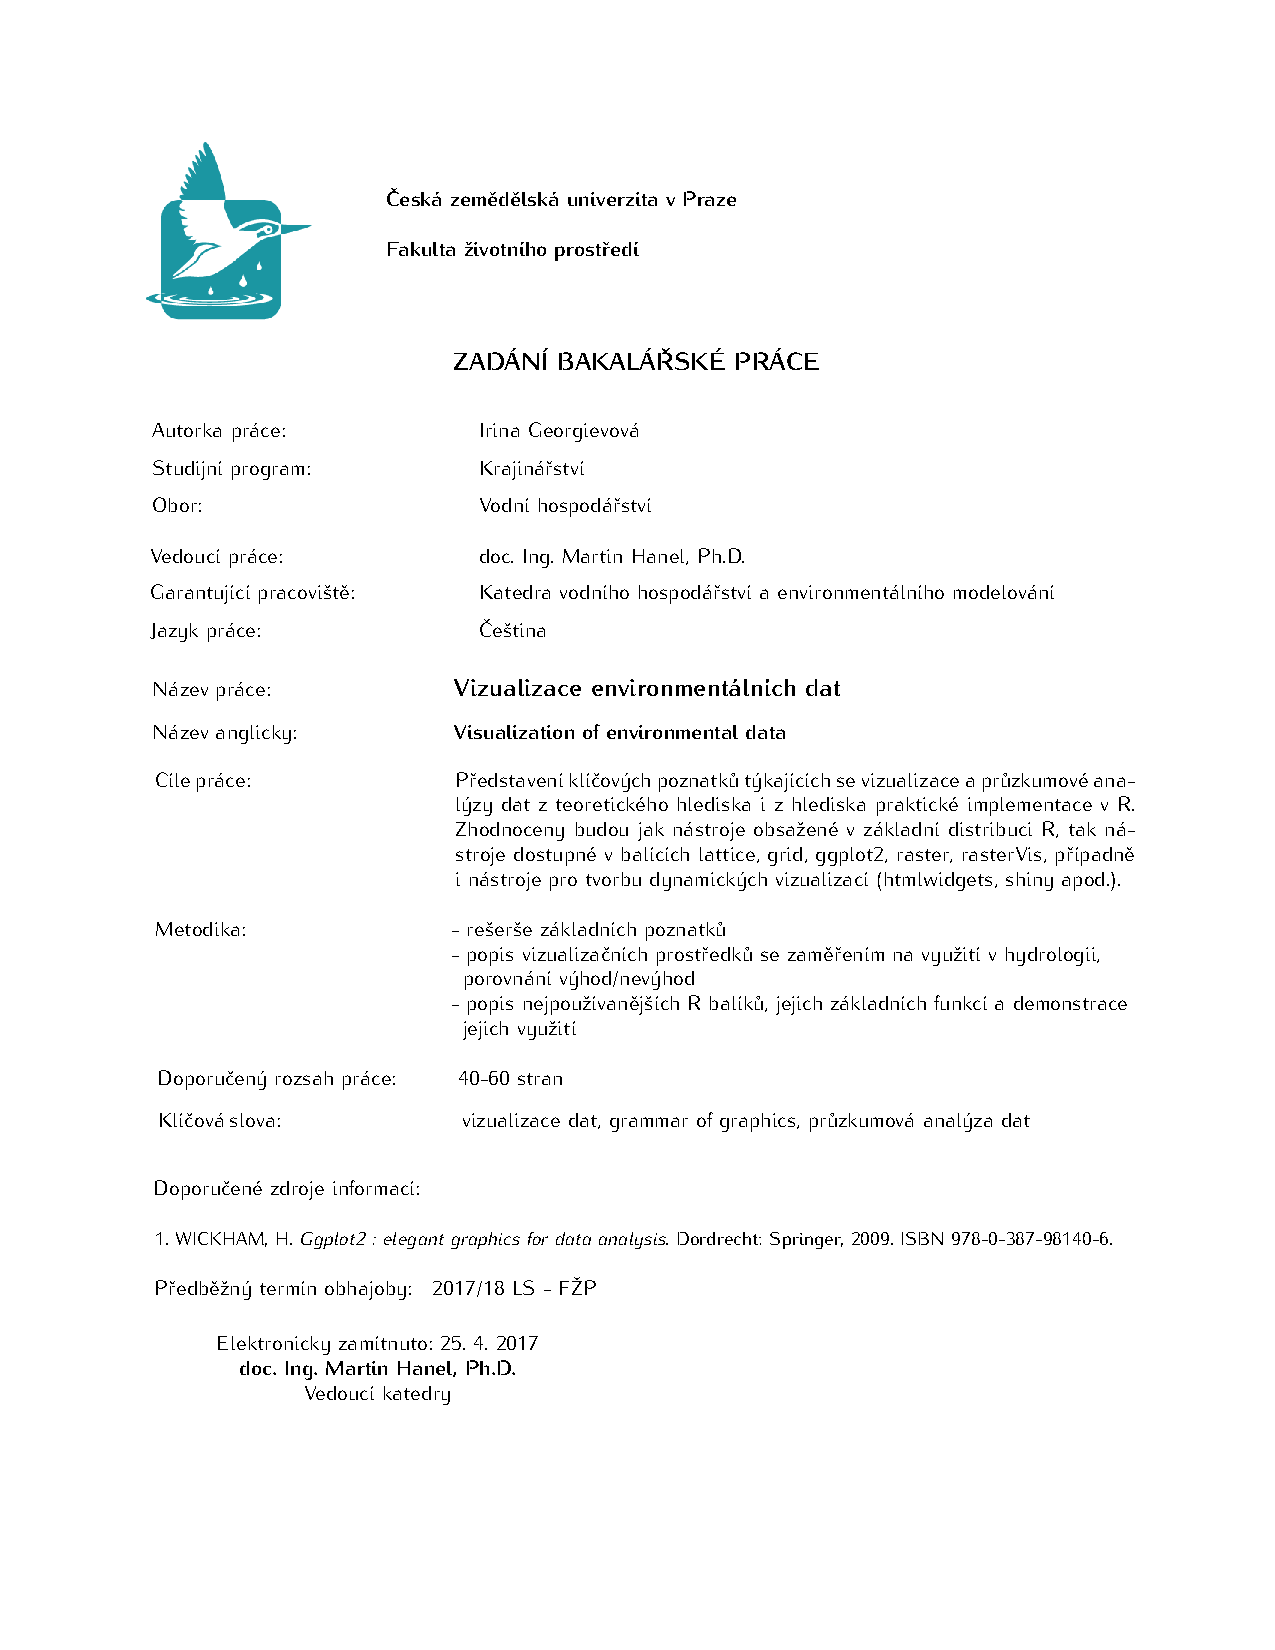
\includepdf[pages={1,2},pagecommand={}, scale = 0.75]{zadani.pdf}
\newpage


\vglue 0pt plus 1fill

\noindent
{\bfseries Prohlášení:} \\
Prohlašuji, že jsem bakalářskou práci \emph{Vizualizace enviromentálních dat} zpracovala samostatně. Veškerou literaturu a další podkladové materiály uvádím v~ seznamu na straně ~\pageref{literatura}.

\vspace{10mm}

\hbox{\hbox to 0.5\hsize{%
V Praze dne ..................
\hss}\hbox to 0.5\hsize{%
\hspace{100pt}...........................
\hss}}

\vspace{1mm}
\hbox{\hbox to 0.5\hsize{%

\hss}\hbox to 0.5\hsize{%
\hspace{100pt}Irina Georgievová
\hss}}

\vspace{20mm}

\newpage

\vglue 0pt plus 1fill
\noindent
{\bfseries Poděkování:} \\

\newpage

\newpage


\vbox to 0.5\vsize{
\setlength\parindent{0mm}
\setlength\parskip{5mm}

{\LARGE\bfseries Abstrakt} 

Práce shrnuje důležité poznatky o vizualizaci dat. Probírá historii jejího vývoje vizualizace a položení vědeckých základů Williamem S. Clevelandem, Edwardem Tuftem a Lelandem Wilkinsonem.  Vizualizace dat je klíčovým nástrojem pro průzkumovou analýzu dat, který je využíván pro jejich lepší pochopení, odhalení neočekávaného chování dat či při rozhodnutí o dalším směru analýzy. Práce dále popisuje nástroje současné  vizualizace dat v programovacím jazyku R a probírá jak základní možnosti softwaru, tak i pokročilé balíčky (\texttt{grid}, \texttt{lattice}, \texttt{ggplot2}, \texttt{raster} a další). Hlavním přínosem práce je tvorba webové aplikace pomocí nástrojů pro dynamickou vizualizací (\texttt{htmlwidgets}, \texttt{Shiny} a \texttt{flexdashboard}).  Aplikace se soustředí na analýzu hydrologické bilance a předpověď sucha v útvarech povrchových vod České republiky a demonstruje veškeré výhody moderní vizualizace dat. 

{\bfseries Klíčová slova: } vizualizace dat, grammar of graphics, průzkumová analýza dat, R, Shiny
\vss}\nobreak\vbox to 0.49\vsize{
\setlength\parindent{0mm}
\setlength\parskip{5mm}
{\LARGE\bfseries Abstract} 



{\bfseries Keywords:  } Data visualization, grammar of graphics, exploratory data analysis, R, Shiny
\vss}

\end{document}


\tableofcontents
\newpage

\section{Úvod}\label{uvod}

\pagestyle{plain} \setcounter{page}{1}

\newpage

\section{Cíle práce}\label{cile-prace}

\newpage

\section*{Teoretická část}\label{teoreticka-cast}
\addcontentsline{toc}{section}{Teoretická část}

\subsection{1 Vizualizace dat}\label{vizualizace-dat}

\subsubsection{1.1 Historie vizualizace
dat}\label{historie-vizualizace-dat}

\qquad Do 17. století jediné, co by se dalo klasifikovat jako
vizualizace dat byly mapy pro navigaci a průzkum, ale také diagramy,
geometrická schémata a tabulky pozic hvězd a jiných nebeských těles.
Postupný vývoj statistické teorie a růst zájmu o data na konci 18.
století vedly k inovacím a expanzi nových grafických forem. Kartografové
se pokoušeli zaznamenat více, než pouhou geografickou polohu na mapě a
objevily se první pokusy o tematické mapování geologických, ekonomických
a medicínských dat.

\qquad Wiliam Playfair (1759-1823) je obecně znám jako průkopník v
oblasti vizualizace dat a je považován za vynálezce několika typů grafů.
Například liniový a sloupcový graf či grafy časových řad byly popsány v
jeho atlasu z roku 1786
\textit{"Commercial and Political Atlas"}\footnote{\textit{"Commercial and Political Atlas: Representing, by Copper-Plate Charts, the Progress of the Commerce, Revenues, Expenditure, and Debts of England, during the Whole of the Eighteenth Century"}}.
Později popsal i koláčový graf ve svém breviáři
\textit{"Statistical Breviary"} z roku 1801. Obrázek \ref{fig0} ukazuje
příklad jeho kreativní kombinace různých vizualizačních technik (kruhy,
koláče, linie), pomocí kterých se snažil porovnat daňovou zátěž mezi
Británii a dalšími zeměmi. Na tomto grafu také ukázal možnost použití
více měřítek pro různé ukazatele (graficky vyjádřena populace a výše
daní).

\begin{figure}[H]

{\centering \includegraphics[width=1\linewidth]{fig/Playfair_taxes_population} 

}

\caption{\label{fig0} Kombinace různých vuzuálních techník, Playfair 1801}\label{fig:playfair}
\end{figure}

\newpage

\begin{wrapfigure}[16]{R}{0.45\textwidth}
    \centering
    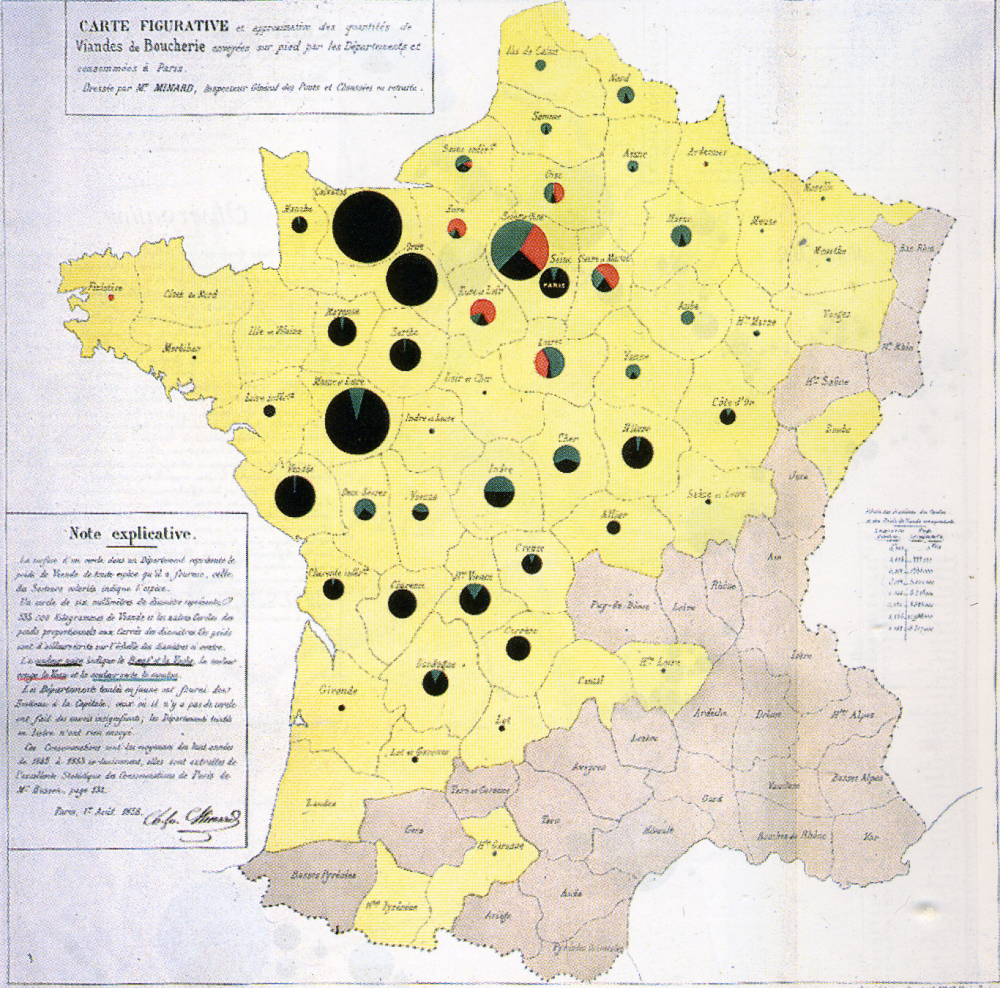
\includegraphics[width=0.42\textwidth]{fig/Minard_1858}
    \vspace{-5pt}
    \caption{Dobytek odeslaný z celé Francie ke spotřebě v Paříži, Minard 1858}
    \label{fig01}
\end{wrapfigure}

\qquad V polovině 19. století byly vytvořeny všechny podmínky pro rychlý
růst vizualizace. V důsledku rostoucí významnosti číselných informací
pro sociální plánovaní, industrializaci, obchod a dopravu byly zřízeny
oficiální statistické úřady po celé Evropě. Rozvoj statistické teorie,
iniciovaný Johannem Carlem Friedrichem Gaussem a Pierrem Simonem de
Laplacem, měl odezvu ve společností a poskytl prostředky ke zpracování
velkého množství dat. Pro vizualizaci dat se stalo období 1850-1900
\enquote{zlatým věkem}, s velkým množstvím inovací. S těmito inovacemi
je hlavně spojeno jméno Charlese Josepha Minarda {[}1781-1870{]}.
Minardem bylo například zavedeno použití koláčových grafů s výsečemi na
mapách (obrázek \ref{fig01}), kde velikost koláčového grafu ukazuje sumu
sledované proměnné pro každou oblast na mapě a výseče reprezentují dílčí
součty za jednotlivé kategorie. Dále se také zabýval znázorněním
geografických pohybů úměrně jejich velikostí jako je přeprava lidí,
zboží, import či export. Tento typ vizualizace se nazývá
\textit{"flow maps"}, viz obrázek \ref{fig02}. Jednou z jeho
nejslavnějších prací je zobrazení postupných ztrát francouzské armády
během Napoleonského tažení na Moskvu v letech 1812-1813 (obrázek
\ref{fig03}). Je považována za nejlepší informativní vizualizaci vůbec.
I přestože v~tomto grafu je celkem 6 proměnných (množství, lokace ve
dvou rozměrech, postup armády, teplota, datum a~skupiny), podařilo vše
zobrazit tak, aniž by graf byl přeplněný a~\mbox{matoucí.}

\begin{wrapfigure}[12]{L}{0.51\textwidth}
    \centering
    \vspace*{-20pt}
    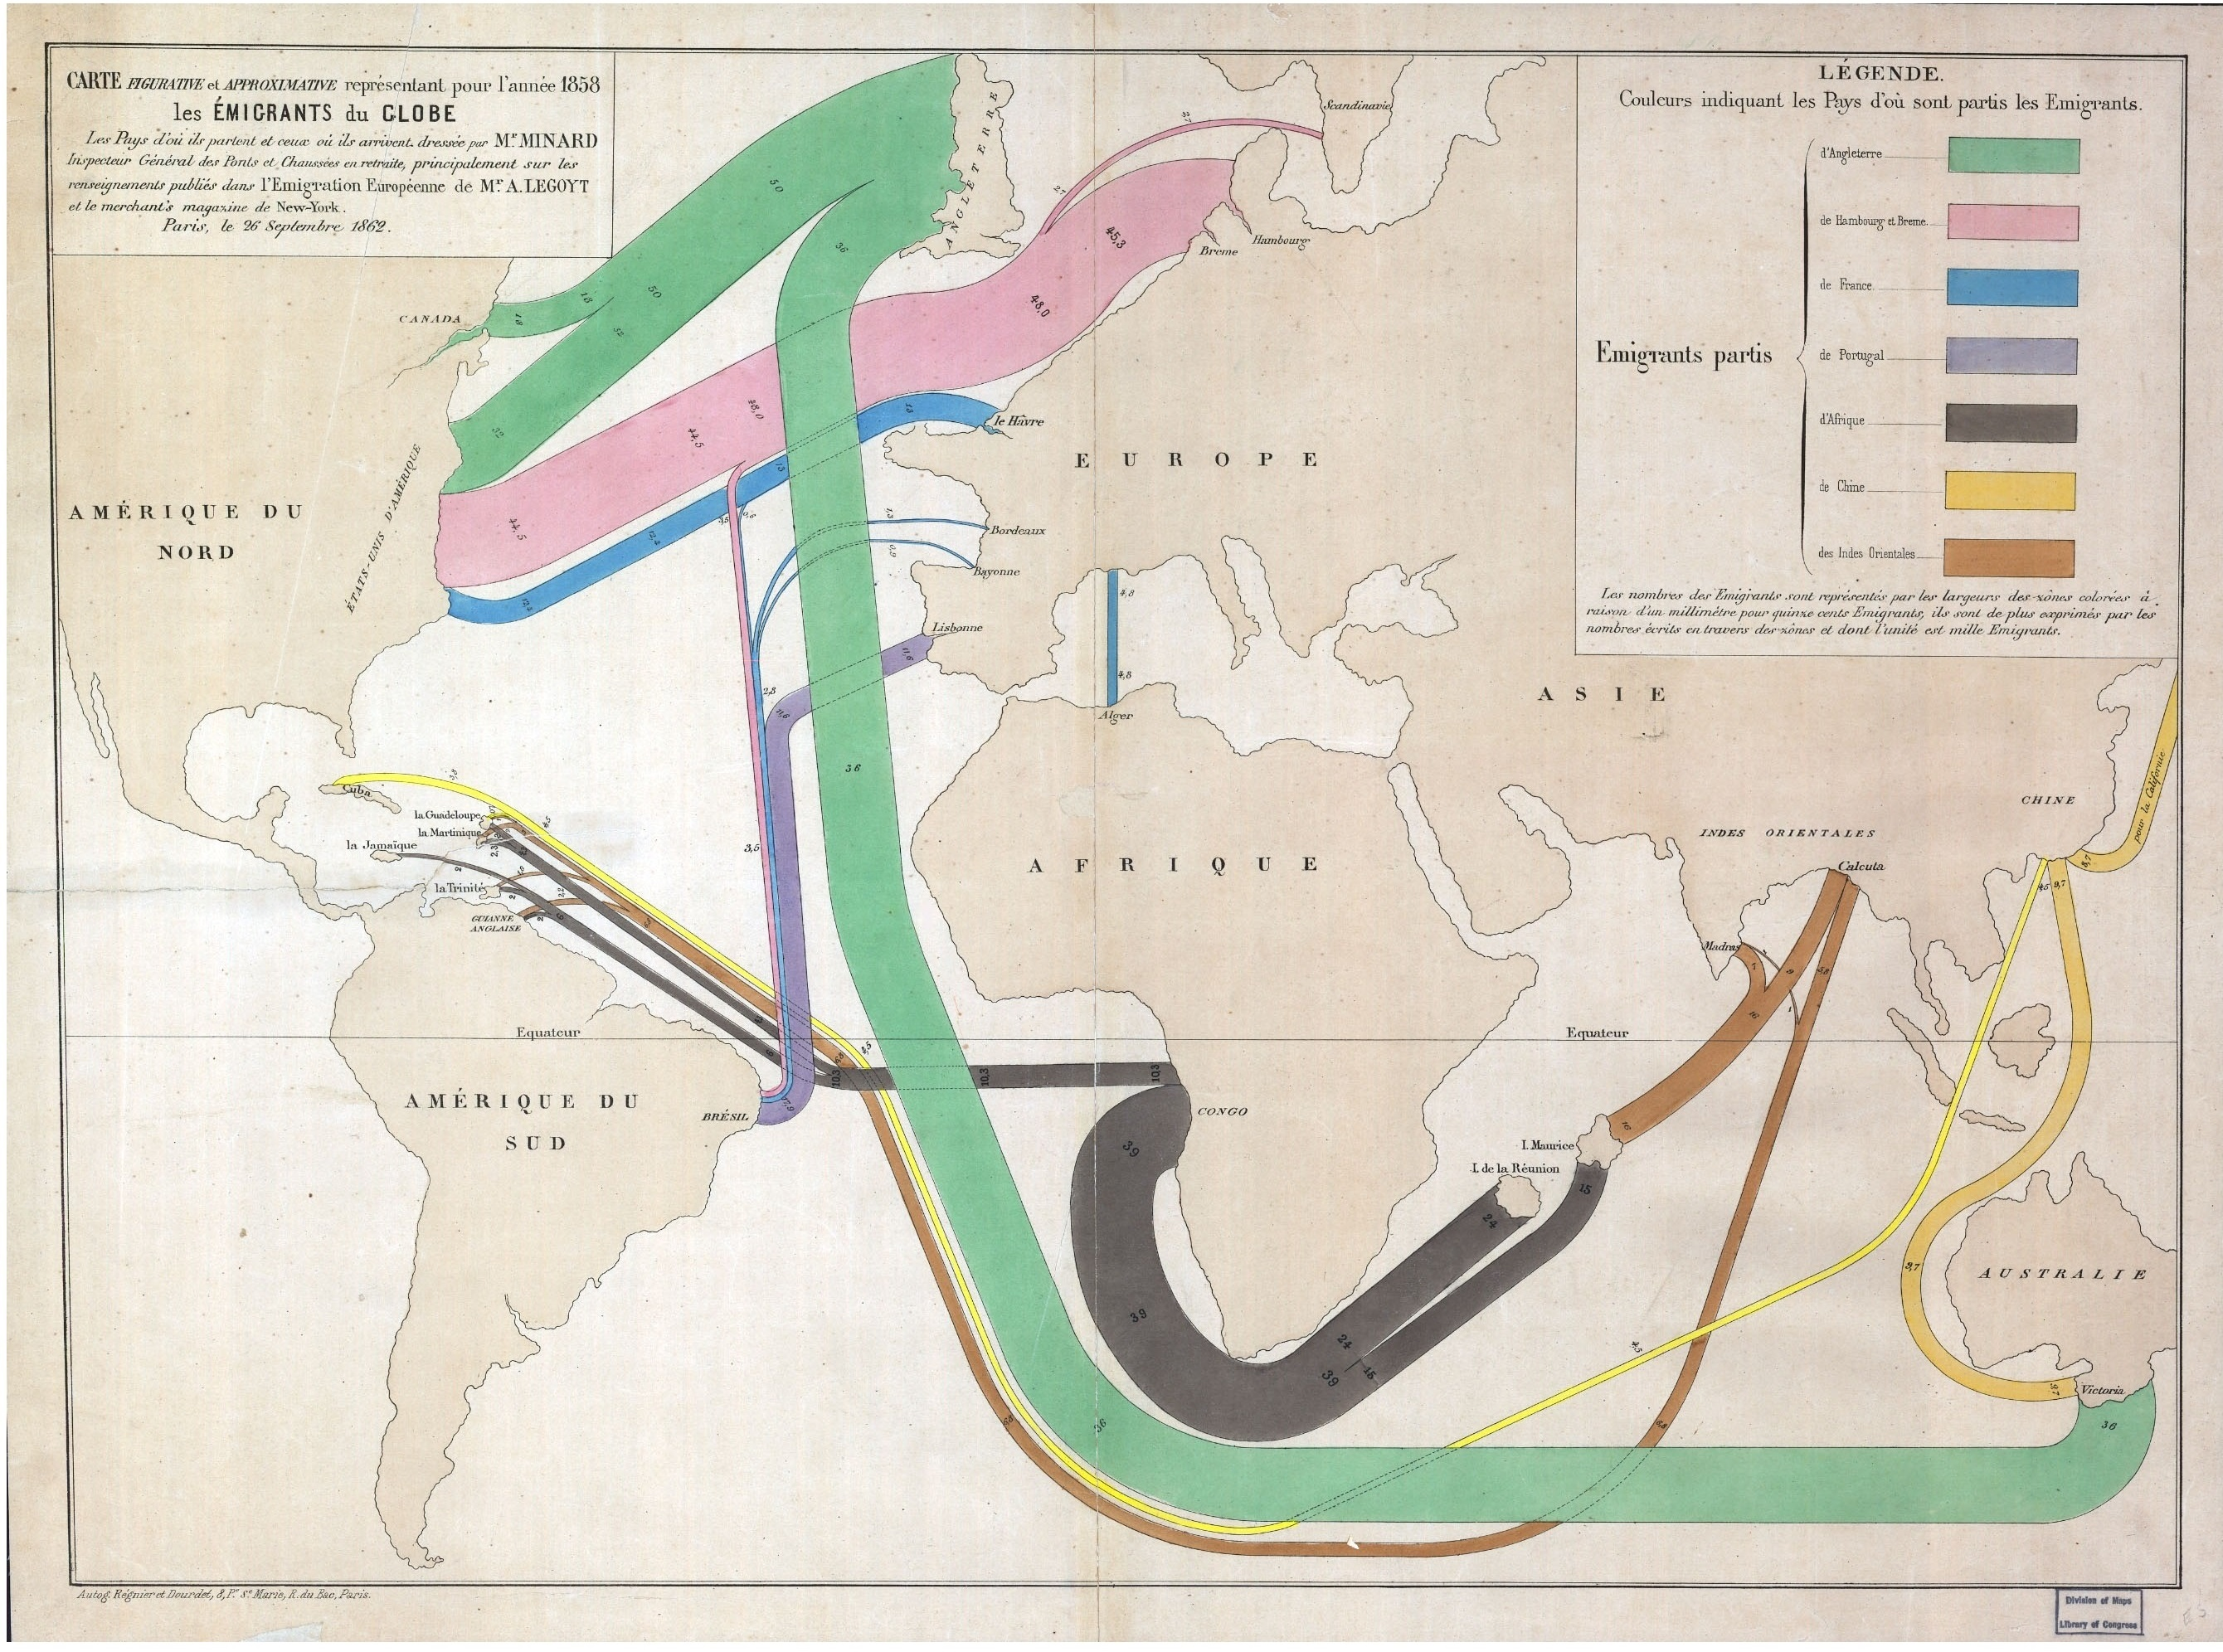
\includegraphics[width=0.5\textwidth]{fig/minard_flow_map.jpg}
    \vspace{-5pt}
    \caption{Mapa světové migrace, Minard 1858}
    \label{fig02}
\end{wrapfigure}

\vspace{2.5pt} \qquad Začátek 20. století je občas nazýván
\enquote{moderním temným věkem} vizualizace. V letech 1900-1950 bylo jen
málo inovací. Nadšení pro vizualizací, které charakterizovalo 19.
století bylo nahrazeno formálními (z velké části statistickými) grafy a
modely z oblasti sociologie. Hlavní zájem byl o přesná čísla, odhady
parametrů a směrodatné odchylky. Vizualizace byla považována za pouhé
hezké obrázky bez schopnosti podat přesná data. {[}1{]}

\begin{figure}[H]
\centering
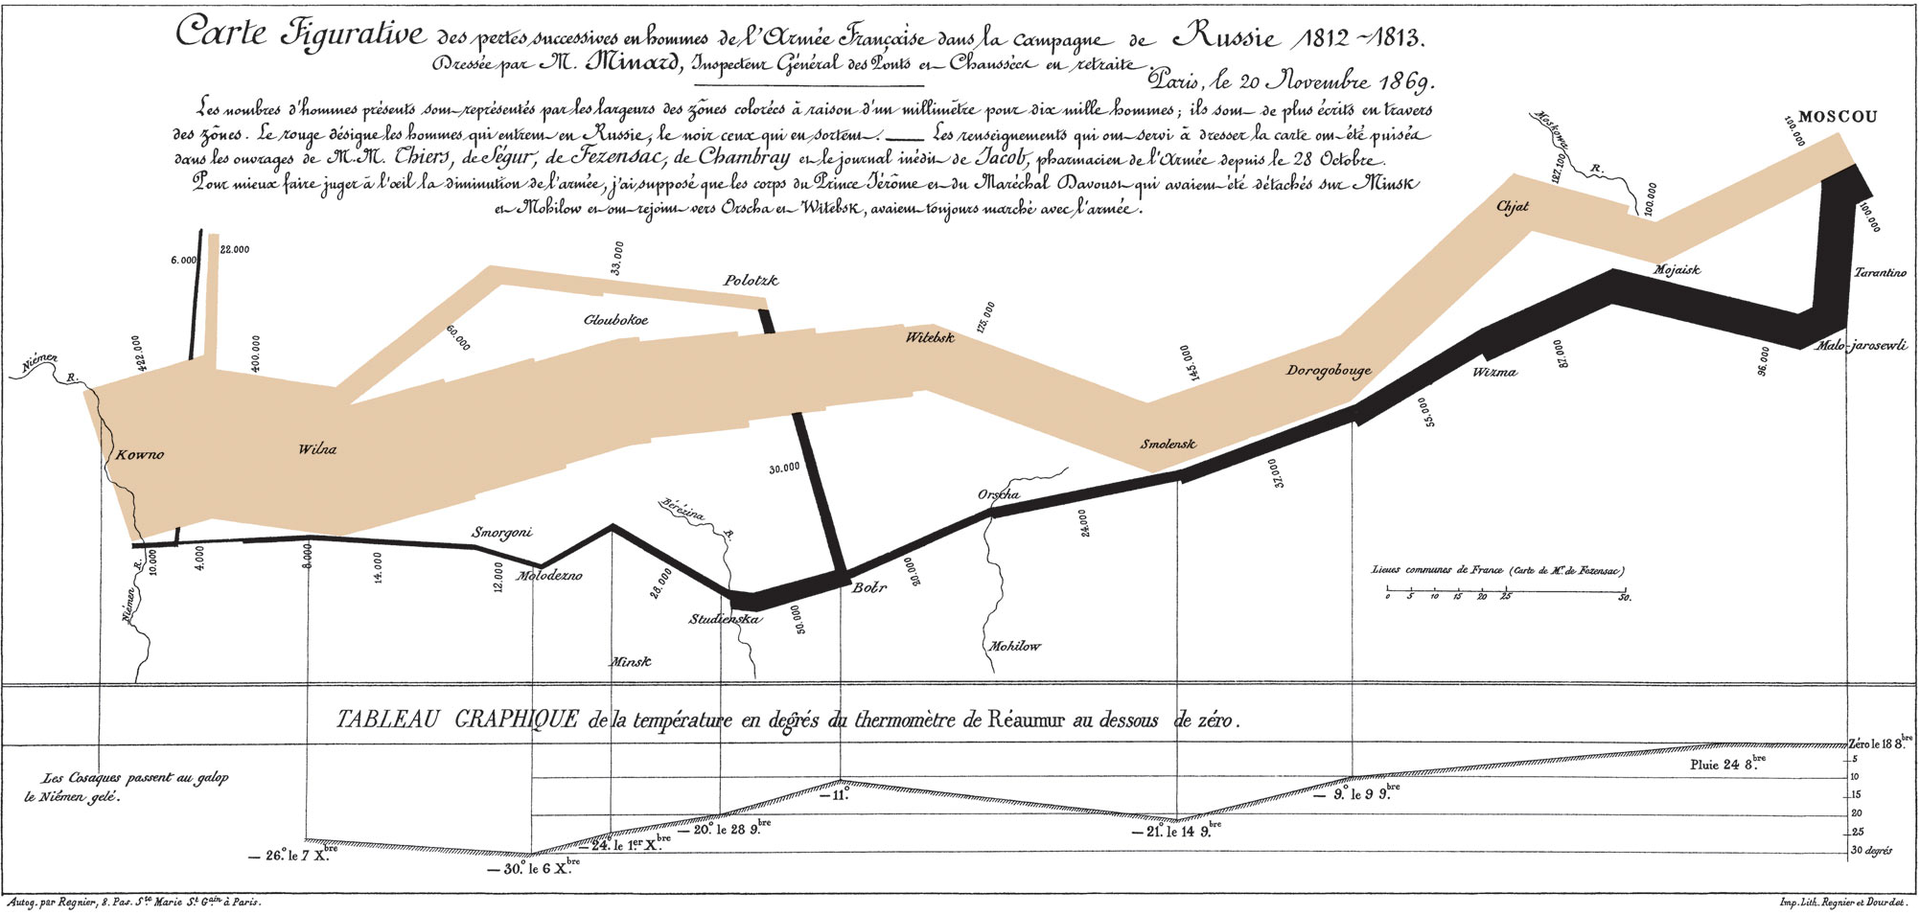
\includegraphics[width = \textwidth]{fig/Minard_1869}
\caption{Postup Napoleonských vojsk v letech 1812-13, Minard 1869}
\label{fig03}
\end{figure}

\qquad Ve své knize \textit{"Graphic Methods for Presenting Facts"} z
roku 1919 Willord C. Brinton {[}1880-1957{]} kritizoval a vysvětloval
chyby takovýchto grafů. Například koláčový graf rozdělení rodinných
příjmů (od 900\$ do 1000\$) na obrázku \ref{fig04}. Tento graf je
příkladem nepovedené vizualizace: oko preferenčně soudí dle velikostí
obrázků a ne dle uhlů výsečí. Obrázek uprostřed znázorňuje druhy
utracení: je to zábavný způsob vizualizace, avšak nelze přesně určit
velikost brašen, ani je porovnat mezi sebou. Další obrázek by měl
čtenáři sdělit informaci, že prodej praček za poslední tří roky vzrostl
sedmkrát. Z obrázku není patrný poměr sedmi ku jedné ani přesné roky kdy
bylo provedeno porovnání údajů. Dále Brinton ve své práci upozorňoval,
že neúspěšná prezentace dat může vést k chybným závěrům a také zmiňoval
potřebu jakéhosi standardu, souhrnu \enquote{gramatických pravidel pro
grafický jazyk}. {[}2{]}

\begin{figure}[H]

{\centering 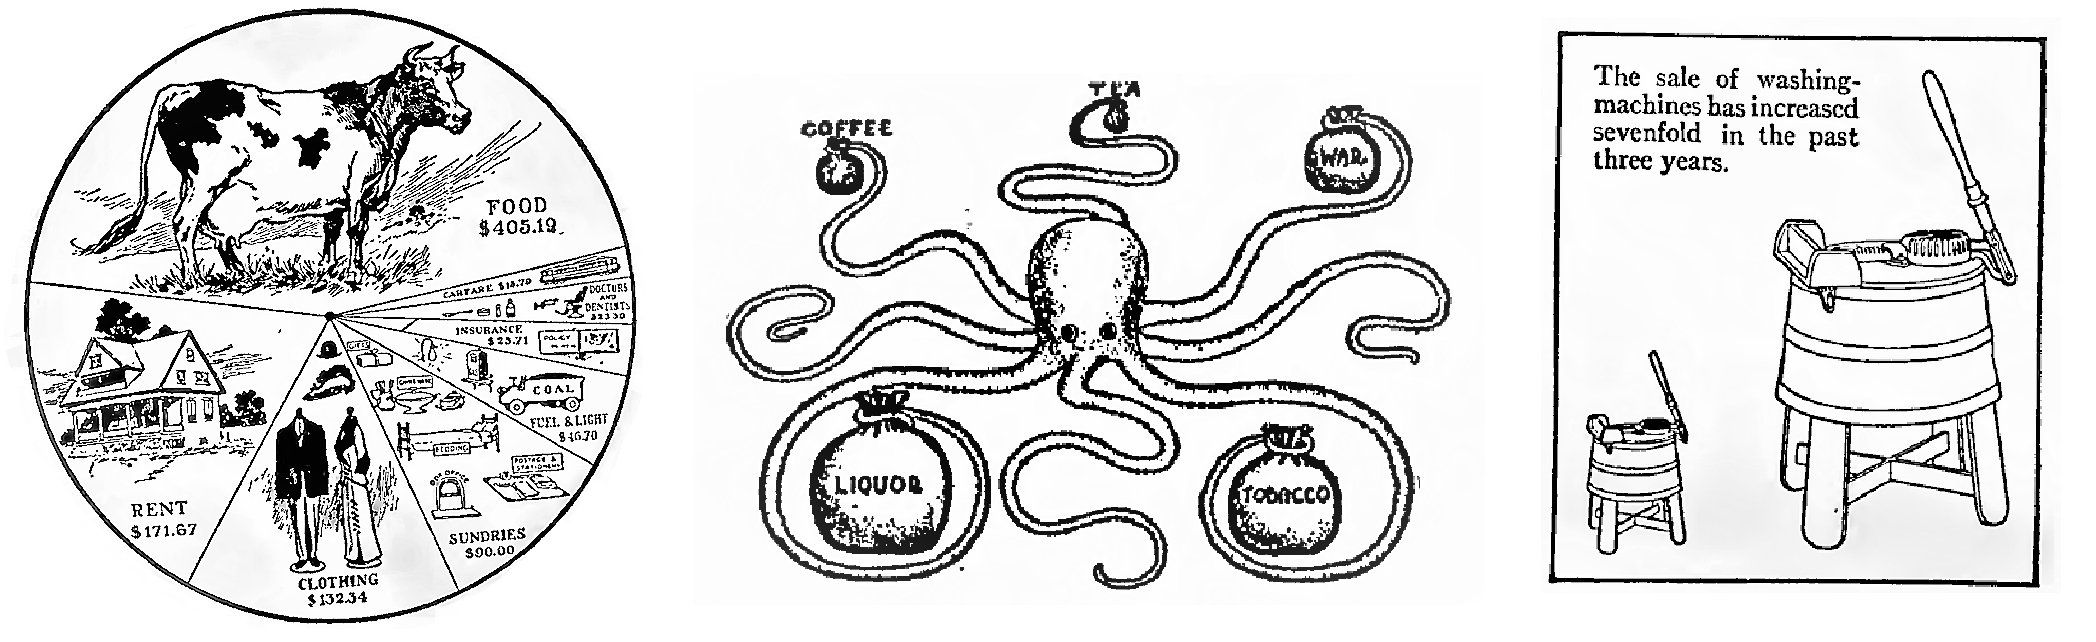
\includegraphics[width=1\linewidth]{fig/brinton} 

}

\caption{\label{fig04} Ukázky vizualizací ze začátku 20. století, Brinton 1919}\label{fig:brinton}
\end{figure}

\newpage

\qquad Ke \enquote{znovuzrození} vizualizace došlo v polovině šedesátých
let 20. století po zveřejnění článku Johna W. Tukeyho {[}1915-2000{]}
\textit{"The Future of Data Analysis"}, ve kterém vyzývá společnost k
uznání analýzy dat jako samostatného oboru statistiky odlišného od
statistiky matematické. {[}3{]} Brzy poté začal Tukey s vývojem široké
řady nových a efektivních grafů pod společným názvem \enquote{průzkumová
analýza dat} (popsáno v jeho knize \textit{"Explanatory Data Analysis"}
z roku 1977, viz o tématu kapitola~\protect\hyperlink{EDA}{3}).~{[}4{]}
Mezi těmito novými grafy je například číslicový histogram (popsaný
v~kapitole \protect\hyperlink{stem-and-leaf}{2.4.3}), boxplot nebo
krabicový graf (popsaný v kapitole \protect\hyperlink{boxplot}{2.3.2}) a
další. Mnoho z nich je aktivně používáno ve statistické praxi a
implementováno do většiny softwarů.~{[}1{]}

\subsubsection{1.2 Zásady vizualizace dat}\label{zasady-vizualizace-dat}

\qquad Od roku 1975 se vyvíjí statistické výpočetní systémy a s nimi i
nové metody analýzy a vizualizace dat. V tomto období vizualizace začala
být vnímána jako vlastní odvětví a to především díky Williamu S.
Clevelandu a Edwardu Tuftemu, kteří položili vědecké základy tohoto
odvětví. Tufte vyvinul a popularizoval terminologii a základní principy
grafické integrity. Cleveland se zabýval studií grafického vnímání,
kognitivních procesů, které lidé používají k pochopení grafů, a rozvíjel
teorii o správném provedení vizualizace. {[}5{]} Výsledek jejich práce
se promítá i do současné doby kvalitní, interaktivní a dynamickou
vizualizací. {[}1{]}

\hypertarget{tufte}{\paragraph{1.2.1 Edward Tufte}\label{tufte}}

\qquad Za revoluční průlom se považuje kniha Edwarda Tufte \emph{The
Visual Display of Quantitative Information} z roku 1983, v kombinaci se
dvěma posléze publikovanými knihami \emph{Envisioning Information} a
\emph{Visual Explanations} z roku 1990, resp. 1997, patří mezi
nejznámější publikace na téma vizualizace dat. Právě v těchto
publikacích Tufte originálním způsobem definuje \enquote{standard}
vizualizace. {[}6{]} Ideální vizualizace dle Tufteho je stručná,
elegantní a informativní. Příkladem ideálního grafu je pro Tufteho graf
postupu Napoleonských vojsk v letech 1812-13, vytvořený Minardem (viz
obrázek \ref{fig03}). Tufte říká, že grafická elegance se často nachází
v jednoduchosti návrhu a komplexnosti dat. {[}7{]} Tafte formuluje
základní principy vizualizace jako grafickou dokonalost a grafickou
integritu.

\begin{itemize}
\tightlist
\item
  \textbf{Grafická dokonalost} - grafika by měla:

  \begin{itemize}
  \tightlist
  \item
    být o datech a během jejich reprezentace by nemělo dojít ke
    zkreslení
  \item
    vyvolávat otázky o datech, ne o metodologii a technikách vizualizace
  \item
    ukazovat velké množství dat na malém prostoru
  \item
    podávat velké datasety souvisle a logicky
  \item
    sloužit rozumnému a jasnému cíli (popisu, průzkumu, \(\dots\))
  \item
    být jednotná se statistickým nebo slovním popisem datasetu
  \end{itemize}
\end{itemize}

\newpage

\begin{itemize}
\tightlist
\item
  Pravidla pro \textbf{Grafickou integritu} neboli grafickou celistvost
  a jednoznačnost:

  \begin{itemize}
  \tightlist
  \item
    reprezentace čísel zobrazených v grafu by měla být přímo úměrná
    číselným veličinám datasetu
  \item
    jasná, detailní a svědomitá označení v grafech pro potlačení
    zkreslení, nejasností a dvojznačností
  \item
    popisky jsou důležité
  \item
    ukazovat variaci dat, nikoliv designu
  \item
    v případě časových řad, představujících peníze, používat obecně
    známé jednotky
  \item
    počet rozměrů představených v grafu by neměl přesahovat počet
    proměnných datasetu
  \item
    reprezentace by neměla zahrnovat neúmyslný kontext
  \end{itemize}
\end{itemize}

\begin{minipage}[H]{0.475\textwidth}
 \begin{figure}[H]
\centering
    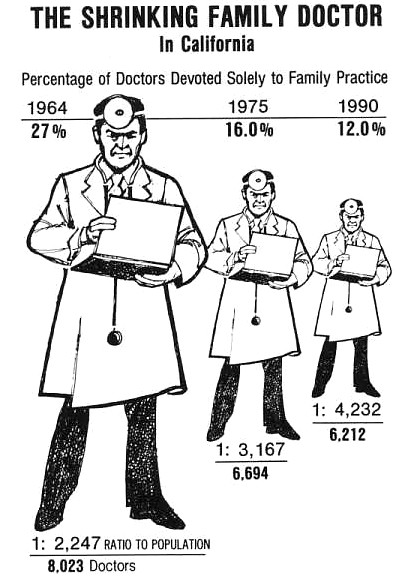
\includegraphics[height = 10.5cm]{fig/tufte_shrinking_doctor}
    \caption{Snižující se procento rodinných lékařů, Los Angeles Times, 1979}
    \label{fig05}
 \end{figure}
\end{minipage}\begin{minipage}[H]{0.05\textwidth}
 
\includegraphics[height = 9cm]{fig/blank_v}
\end{minipage}\begin{minipage}[H]{0.475\textwidth}
 \begin{figure}[H]
\centering
    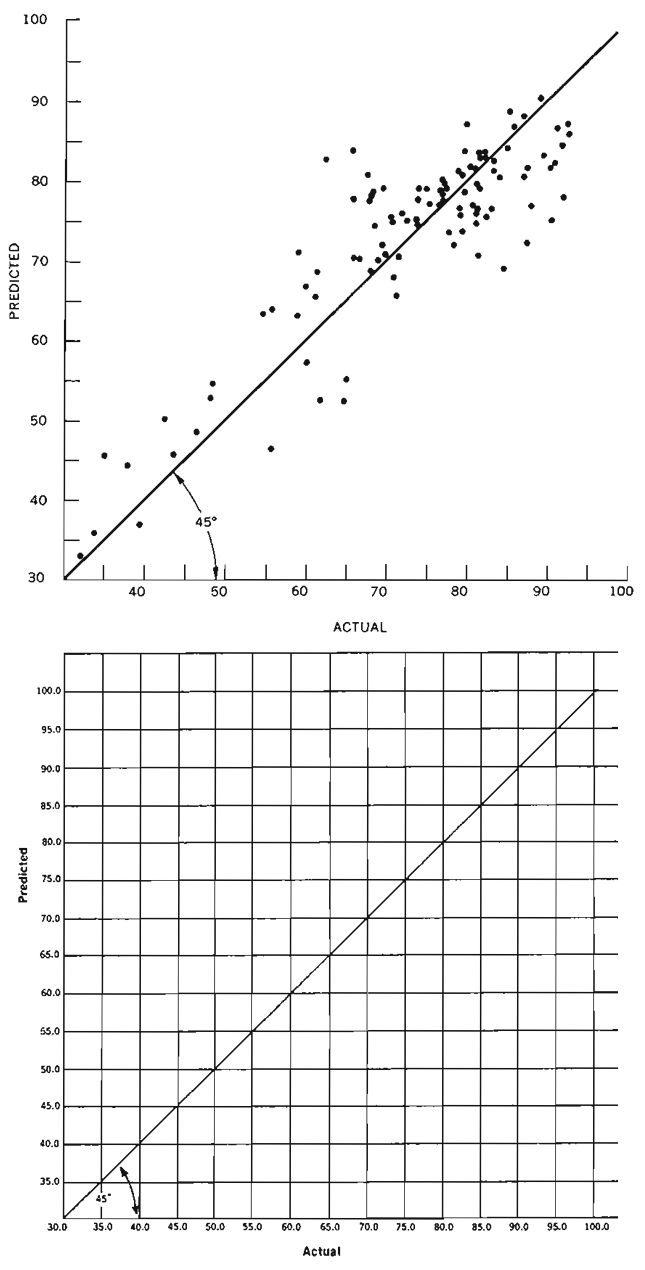
\includegraphics[height = 10.5cm]{fig/data_ink}
    \caption{Vztah skutečné míry volební registrace k předpovídaným hodnotám, převzato E. Tuftem, 1983}
    \label{fig06}
 \end{figure}
\end{minipage}

Ve spojení s těmito principy byly zavedeny Edwardem Tuftem následující
termíny:

\begin{itemize}
\item
  \textbf{Lie factor} je definován jako poměr velikosti efektu
  zobrazeného v grafu oproti velikosti efektu v datech. Pokud se rovná
  jedné, považují se reprezentované hodnoty za přesné. Pokud je faktor
  větší než 1.05 či menší než 0.95, indikuje podstatné zkreslení,
  přesahující míru drobných nepřesností vyskytujících se při
  vykreslování grafu. Tafte ve své práci uvádí jako jeden z příkladů
  graf na obrázku \ref{fig05}. Tento graf zobrazující snižující se
  procento lékařů věnujících se výhradně rodinné praxi má \emph{lie
  factor} odpovídající hodnotě 2.8, tedy skutečný pokles je značně
  nadhodnocen.
\item
  \textbf{Data ink ratio} - poměr, který vyhodnocuje hustotu grafu a
  obsah informací. Dal by se vyjádřit vzorcem
  \[\textit{Data ink ratio} = \cfrac{\textit{data-ink}}{\textit{celkový inkoust použitý v datech}},\]
  kde \(\textit{data-ink}\) je nezbytné jádro grafu a smazání jakékoliv
  jeho části znamená ztrátu informací. Tento vztah také odpovídá podílu
  grafického inkoustu požitého k vykreslení nepodstatných informací.
  Dalo by se to také vyjádřit jako jedna mínus
  \textit{podíl grafiky, která může být vymazána bez ztráty informací}.
  Tafte doporučuje tento faktor maximalizovat v rozumných mezích,
  nejlépe se vyhnout těžkým mřížkovým liniím na pozadí (dokonce i
  horizontálním referenčním liniím). V příkladu na obrázku \ref{fig06}
  jsou zobrazeny dvě verze stejného grafu. Horní má hodnotu \emph{data
  ink ratio} kolem 0.7, dolní graf, však protože neobsahuje informaci o
  datech, pouze nápomocné čáry, má \emph{data ink ratio} roven nule.
\item
  \textbf{Chartjunk} - se vztahuje ke všem vizuálním elementům, které
  neslouží ke komunikaci informací zobrazených v grafu nebo odvádějí
  pozornost od těchto informací. {[}8{]}
\end{itemize}

\hypertarget{cleveland}{\paragraph{1.2.2 Wiliam S.
Cleveland}\label{cleveland}}

\qquad Kromě práce Edwarda Tufte velkýho měly vliv i publikace Wiliama
S. Clevelanda. Cleveland se svým kolegou Robertem McGillem publikovali v
roce 1984 článek o grafickém vnímání {[}9{]}. Prováděli studie
zabývající se rozdílem ve vnímání sloupcových grafů (pozice a obecné
měřítko), koláčových grafů (úhel), skládaných sloupcových grafů
(plocha), barevných a stínovaných map (saturace barev a stínování) a
dalších. {[}5{]} Ve svých knihách \emph{Visualizing data} z roku 1993 a
\emph{The Elements of Graphing Data} z roku 1994 se Cleveland zabýval
principy vizualizace, grafickými metodami a technikami či vykreslením
tří a více proměnných (rozměrů). Některé z jeho principů se shodují s
principy vymezenými Tuftem, avšak výzkum Clevelanda v této oblasti
přesahovala práci Tufteho. Zásady a principy dle Clevelanda by se daly
shrnout do čtyř hlavních kategorií: jasná vize, srozumitelnost, měřítka
a obecné postupy. {[}10{]}

\begin{itemize}
\tightlist
\item
  \textbf{Jasná vize}

  \begin{itemize}
  \tightlist
  \item
    Data by měla vyčnívat, bez vykreslení nadbytečných prvků (neboli
    \emph{chartjunk} dle Tufteho)
  \item
    K zobrazení dat by se měly používat výrazné grafické prvky.
  \item
    Pro každou proměnnou by měla být použita dvojice os, prostor v takto
    vytvořeném obdélníku je určen k vykreslení grafu, značky na osách by
    měly směrovat mimo oblast grafu.
  \item
    Prostor grafu by neměl být přeplněný (legenda mimo oblast grafu
    atd.).
  \item
    S počtem značek na osách by se nemělo přehánět.
  \item
    Pokud je to vhodné, referenční linie mohou být použity, avšak
    nesmějí zasahovat do dat.
  \item
    Popisky by neměly zasahovat do kvantitativních dat a nesmějí
    znepřehledňovat graf.
  \item
    Značky a klíče by měly vyskytovat mimo oblast grafu (případně v
    legendě), totéž se týká poznámek a nadpisů, které mohou být také
    umístěny do textu.
  \item
    Překrývající se data sety či symboly musí být vizuálně snadně
    rozpoznatelné.
  \item
    Jasnost obrazu musí být zachována při reprodukci i při snížení
    kvality a zmenšení rozlišení.
  \end{itemize}
\end{itemize}

Cleveland jako příklad špatně zpracované vizualizace vybral graf
\ref{fig07a}, na kterém je zobrazeno množství izotopu xenonu
\({}^{133}\mbox{Xe}\) ve vzduchu (\(pCi.m^{-3}\)) po havárii elektrárny
Three Mile Island v Albany, ve státě New York koncem března a začátkem
dubna roku 1979. Vše, včetně popisků os, klíčů a popisků dat bylo
umístěno do oblasti grafu, není dodržena žádná ze zásad Clevelanda.
Výsledkem je matoucí graf, který je obtížně čitelný. Stejná data byla
vizualizována Clevelandem na grafu \ref{fig07b} s dodržením veškerých
zásad: odstranění zbytečných objektů a detailů z oblasti grafu, datasety
se zobrazují ve vlastních panelech, oprava popisků popisujících měření.

\begin{figure}[H]
  \begin{subfigure}{0.57\textwidth}
  \centering
    \vspace*{0.65cm}
      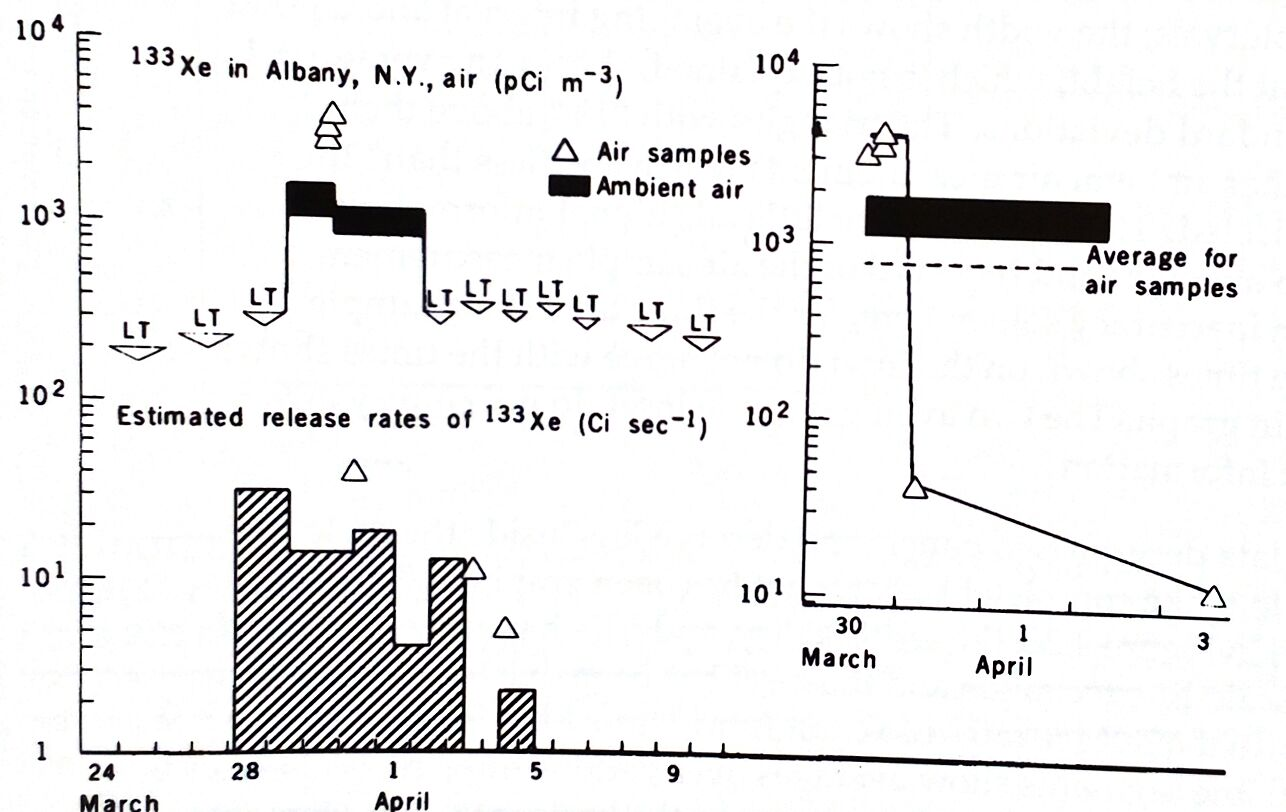
\includegraphics[width=\textwidth]{fig/cleveland_xenon_133}
      \vspace*{0.2cm}
      \caption{}
      \label{fig07a}
  \end{subfigure}%
  \begin{subfigure}[H]{0.43\textwidth}
  \centering
      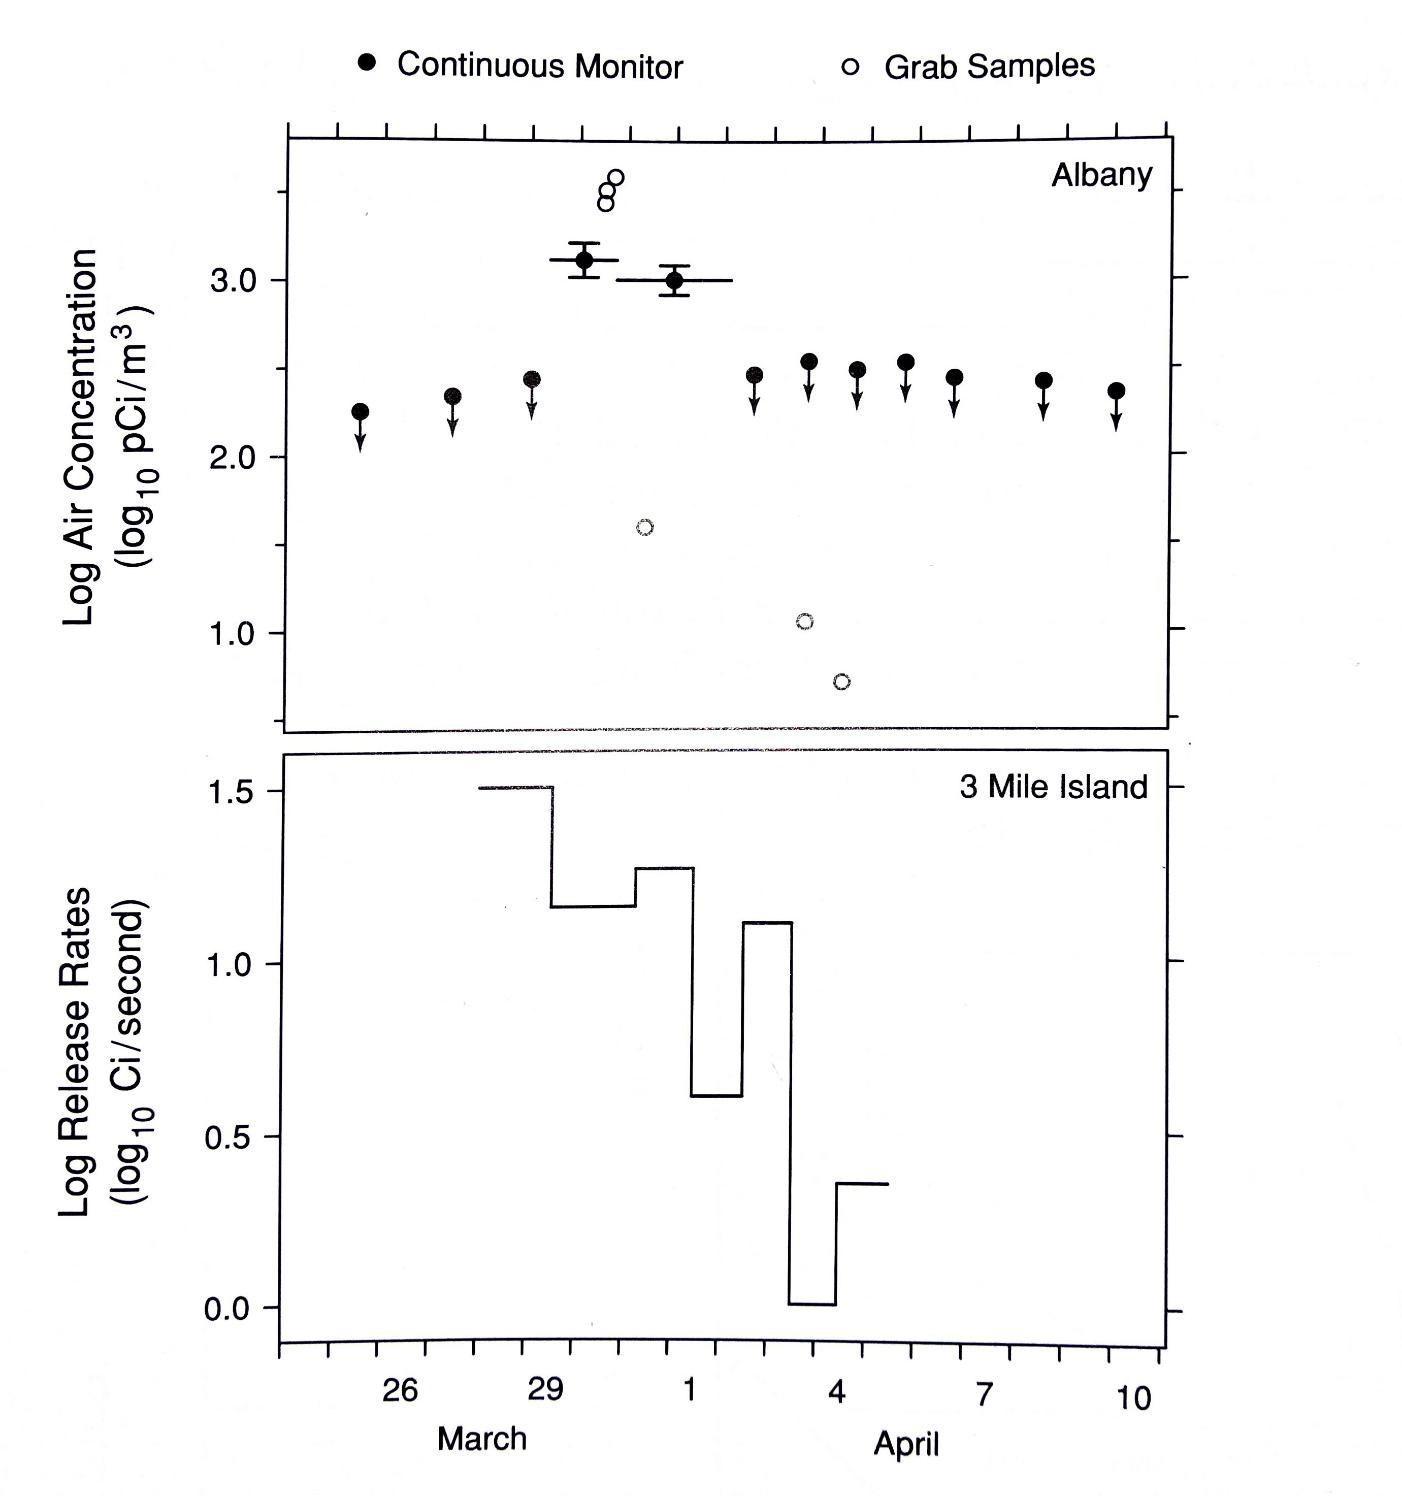
\includegraphics[width=\textwidth]{fig/cleveland_xenon_opr}
      \vspace*{-0.8cm}
      \caption{}
      \label{fig07b}
  \end{subfigure}
\vspace*{-0.25cm}
\caption{Radioaktivní oblak při havárii elektrárny Three Mile Island: ${}^{133}\mbox{Xe}$ ve vzduchu ve vzdálenosti \SI{375}{\kilo\meter} (a) a stejný graf přepracovaný Clevelandem (b), 1994} 
\label{fig07}
\end{figure}

\begin{itemize}
\tightlist
\item
  \textbf{Jasná srozumitelnost}

  \begin{itemize}
  \tightlist
  \item
    Hlavní závěry by měly být obsaženy v grafické formě. Legenda a
    nadpisy by měly být srozumitelné a vyčerpávající.
  \item
    Grafy by měli být zkontrolovány.
  \item
    Mělo by se usilovat o přehlednost (viz \enquote{jasná víze}).
  \end{itemize}
\end{itemize}

\newpage

\begin{itemize}
\tightlist
\item
  \textbf{Měřítka}

  \begin{itemize}
  \tightlist
  \item
    Volit rozsah os tak, aby obsahoval, případně téměř obsahoval, rozsah
    dat.
  \item
    Volit takové měřítko, aby data vyplňovala co největší prostor.
  \item
    Občas je užitečné mít pro proměnnou dvě osy pro rozdílná měřítka.
  \item
    Volit vhodné měřítko pokud data jsou porovnávány na více panelech.
  \item
    Osy grafu nemusejí vždy nutně zahrnovat nulu pro ukázku rozsahu.
  \item
    Použít logaritmická měřítka, když je důležité pochopit procentní
    změny nebo multiplikativní faktory.
  \item
    Použít přerušené měřítko pouze v případě potřeby. Alternativou může
    být logaritmizace měřítka.
  \end{itemize}
\item
  \textbf{Obecné postupy}

  \begin{itemize}
  \tightlist
  \item
    Velké množství kvantitativní informace může být vměstnáno do
    relativně malých oblastí.
  \item
    Tvorba grafů by měla být opakující se, iterativní a experimentální
    činností.
  \item
    Data by měla být vykreslena tolikrát, kolikrát je třeba.
  \item
    Užitečné grafy vyžadují pečlivou a detailní práci.
  \end{itemize}
\end{itemize}

\qquad Cleveland se mimo jiné podílel na tvorbě řady technik pro
prohlížení komplexních datových sad s více proměnnými, kterým se říká
\textit{Trellis Graphics} nebo \textit{Trellis Plots}. Technika obdržela
svůj název \textit{trellis} kvůli obvyklému výsledku řady obdélníkových
grafů, připomínajících zahradní mříž. Na obrázku \ref{fig08} je ukázka
\emph{trellis} grafu, zobrazující údaje o emisích motoru. {[}11{]}

\begin{figure}[H]
\centering
    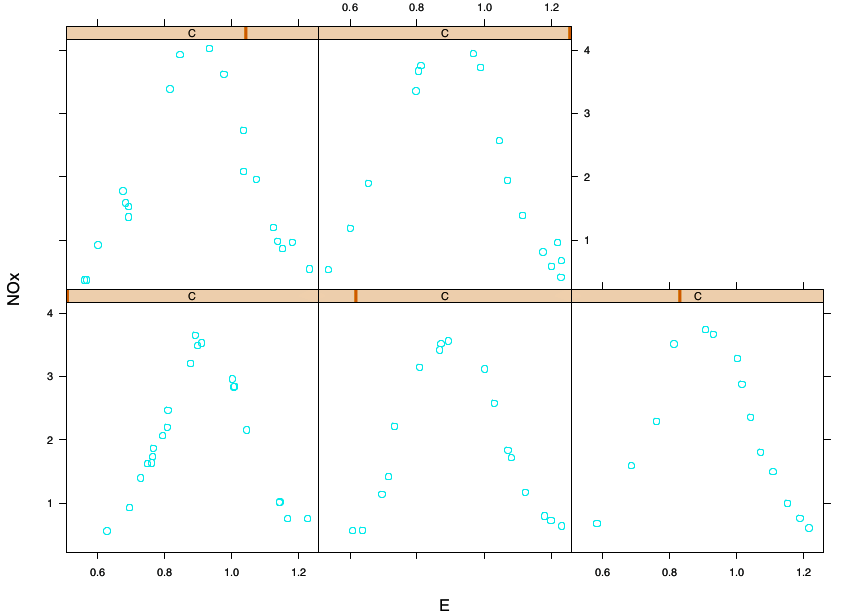
\includegraphics[height = 0.4\textheight]{fig/trellis}
    \caption{\textit{Trellis} graf, zobrazující údaje o emisích motoru, Becker et al., 1996}
    \label{fig08}
 \end{figure}

\newpage

\hypertarget{gg}{\subsubsection{1.3 Grammar of graphics}\label{gg}}

\vspace*{-0.35cm} \qquad \textit{The Grammar of Graphics} publikována
Lelandem Wilkinsonem v roce 2005 {[}12{]} detailně popisuje prvky, které
tvoří základ všech statistických grafů a odpovídá na základní otázku: co
je statistická grafika? {[}13{]} Tato publikace měla extrémně velký vliv
na myšlení o grafech. Hadley Wickham na základě Wilkinsonovy gramatiky
publikoval v roce 2009 článek \emph{A Layered Grammar of Graphics}
{[}14{]}, který se zaměřuje primárně na vrstvy a jejich zapojení do
jazyka R. Následně také pro něj posloužila jako inspirace pro tvorbu
balíčku \texttt{ggplot} (viz kapitola
\protect\hyperlink{ggplot}{4.2.1}).

\qquad \textit{The Grammar of Graphics} říká, že statistická grafika je
mapováním dat k estetickým atributům (barva, tvar, velikost)
geometrických objektů (body, linie, sloupce). Graf také může obsahovat
statistickou transformaci dat a být vykreslen ve specifickém
souřadnicovém systému. \emph{Faceting} může být použito k vygenerování
stejného grafu pro různé podmnožiny datasetu. Kombinace těchto
nezávislých komponent tvoří grafiku. Jednotlivé komponenty tvořící graf,
dle Wilkinsonovy syntaxe, lze zapsat následovně:

\begin{itemize}
\tightlist
\item
  Vizualizovaná \textbf{data} a soubor estetických mapování
  (\textbf{mapping}s) popisujících jak jsou proměnné z dat mapovány na
  vnímané estetické atributy.
\item
  Geometrické objekty (\textbf{geom}s) reprezentují to, co je doopravdy
  na grafu: body, linie, polygony atd.
\item
  Statistické transformace (\textbf{stat}s) sumarizují data mnoha
  užitečnými způsoby. Jako příklad by se daly použít výpočty intervalů a
  počty pozorování při tvorbě histogramu (kapitola
  \protect\hyperlink{hist}{2.4.1}) nebo tvorba lineárního modelu.
  Statistické transformace patří k nepovinným, ale velmi užitečným
  komponentům.
\item
  Měřítka (\textbf{scale}s) reprezentují hodnoty v datovém prostoru
  převedené na hodnoty v estetickém prostoru, ať už se jedná o barvu,
  velikost či tvar. Na měřítku závisí legenda a osy, tvořené inverzním
  mapováním umožňující číst z grafu původní hodnoty datasetu.
\item
  Souřadnicový systém (\textbf{coord}) popisuje, jak jsou souřadnice dat
  mapovány do roviny grafiky. Rovněž poskytuje osy a mřížky, umožňující
  čtení grafů. Běžně se používá kartézský souřadnicový systém, ale je k
  dispozici i řada dalších systémů včetně polárních souřadnic a mapových
  projekcí.
\item
  Specifikace \textbf{facet}ing popisuje, jaké proměnné by měli být
  použity k rozdělení dat na podmnožiny a jak tyto podmnožiny by měly
  být uspořádány. Jedná se o mocný nástroj pro zkoumání toho, zda jsou
  modely stejné nebo odlišné v různých podmínkách.
\end{itemize}

\qquad Je také důležité zmínit, o čem Wilkinsova gramatika není.
Nenaznačuje jaký typ grafů by se měl použít k zodpovězení otázek o
datech, jak to dělali Cleveland {[}15{]} nebo Tukey {[}4{]}, zaměřuje se
konkrétně na jejich tvorbu. Ironií je, že
\textit{The Grammar of Graphics} neurčuje, jak by měla vypadat grafika,
nespecifikuje velikost písma ani barvu pozadí. {[}13{]} Otázkou vzhledu
grafů se zabývali Tufte a Cleveland (kapitoly
\protect\hyperlink{tufte}{1.2.1} a
\protect\hyperlink{cleveland}{1.2.2}). Dále Wilkinsova gramatika
nepopisuje interaktivní ani dynamické vizualizace, obsahuje pouze
statické grafy. Při tvorbě dynamických či interaktivních grafů je třeba
se obrátit na jiný zdroj, například \emph{Interactive Data Visualization
for the Web} od Scottea Murrayho {[}16{]} nebo \emph{Interactive
Visualization} od Billa Ferstera~{[}17{]}. \newpage

\hypertarget{base}{\subsection{2 Základní grafy v R}\label{base}}

\qquad Pro vytváření základních grafů v R používáme vestavěný balíček
\texttt{graphics} {[}18{]}, který obsahuje mnoho užitečných funkcí pro
tvorbu grafických prvků. První kapitola se soustředí na tyto funkce
tohoto balíčku a~v~dalších kapitolách jsou popsány funkce balíčků
dalších (například \texttt{lattice}, \texttt{ggplot2},\ldots{}), které
zastávají podobné funkce, avšak s různým rozsahem nastavení {[}19{]}.

\qquad V následujících příkladech nejsou grafy doplněny o barvy, popisky
os, legendy ani názvy a to především proto, že záměrem této kapitoly je
popsat základní grafy a funkce pro jejich tvorbu v prostředí R. Všechny
tyto prvky mohou být přidány do grafu, ale tím by příkazy obsahovali
irelevantní parametry vzhledem k zaměření této kapitoly. Základní funkce
\texttt{plot(x)} jejímž voláním se obdrží pole s grafickou reprezentaci
proměnné \enquote{x}, by při doplnění kódu o veškeré parametry vypadala
následovaně {[}19{]}:

\begin{Shaded}
\begin{Highlighting}[]
\KeywordTok{plot}\NormalTok{(x, }\DataTypeTok{main =} \StringTok{"Název grafu"}\NormalTok{, }\DataTypeTok{xlab =} \StringTok{"popis osy x"}\NormalTok{, }
\OperatorTok{+}\StringTok{    }\DataTypeTok{ylab =} \StringTok{"popis osy y"}\NormalTok{, }\DataTypeTok{col =} \KeywordTok{c}\NormalTok{(}\StringTok{"red"}\NormalTok{, }\StringTok{"black"}\NormalTok{, }\StringTok{"green"}\NormalTok{)) }
\end{Highlighting}
\end{Shaded}

Záměrem je tedy používání příkazů s pouze relevantními parametry.

\hypertarget{scatterplot}{\subsubsection{2.1 Bodový
graf}\label{scatterplot}}

\qquad Bodový graf je rychlým způsobem, jak znázornit vztahy a
souvislosti mezi proměnnými datasetu, případně k zjištění jejich
neexistence. Data jsou zobrazeny v~kartézském souřadném systému a mají
pro každou hodnotu proměnné dané místo na vodorovné a svislé ose. V
případě existence závislostí mezi proměnnými lze tuto závislost
interpolovat přímkou, křivkou či dalším vhodným vyobrazením této
závislosti.

\qquad Pro vytvoření bodového grafu v základním prostředí R (pomocí
\texttt{graphics}) použijeme funkci \texttt{plot()}, která má tento typ
grafu předdefinovaný pro numerické hodnoty. Viz obrázek \ref{fig1} (a).
Nečíselná data vytvoří jiný typ grafu.

\begin{Shaded}
\begin{Highlighting}[]
\KeywordTok{plot}\NormalTok{(cars)}
\end{Highlighting}
\end{Shaded}

\subsubsection{2.2 Liniový graf}\label{liniovy-graf}

\qquad Jediný rozdíl mezi bodovým a liniovým grafem je, že jeden
zobrazuje body a~druhý je spojuje.{[}19{]} (viz. obrázek \ref{fig1} (a),
(b)). Pro vykreslení liniového grafu se používá již několikrát zmíněná
funkce \texttt{plot()}, kterou doplníme o požadovaný typ vykreslení:

\begin{Shaded}
\begin{Highlighting}[]
\KeywordTok{plot}\NormalTok{(x, }\DataTypeTok{type=}\StringTok{"l"}\NormalTok{)}
\end{Highlighting}
\end{Shaded}

V tabulce \ref{tab1} jsou uvedené některé základní atributy parametru
\texttt{type}, které mohou být použity {[}20{]}:

\begin{table}[H]
\centering
\begin{tabular}{@{}ccc@{}}
\toprule
  & Anglický popis & Český popis    \\ \midrule
p & points         & bodový         \\
l & lines          & liniový        \\
b & both           & složený        \\
h & histogram      & histogram      \\
n & no plotting    & bez vykreslení \\ \bottomrule
\end{tabular}
\caption{Základní atributy parametru `type`}
\label{tab1}
\end{table}

\begin{figure}[H]

{\centering 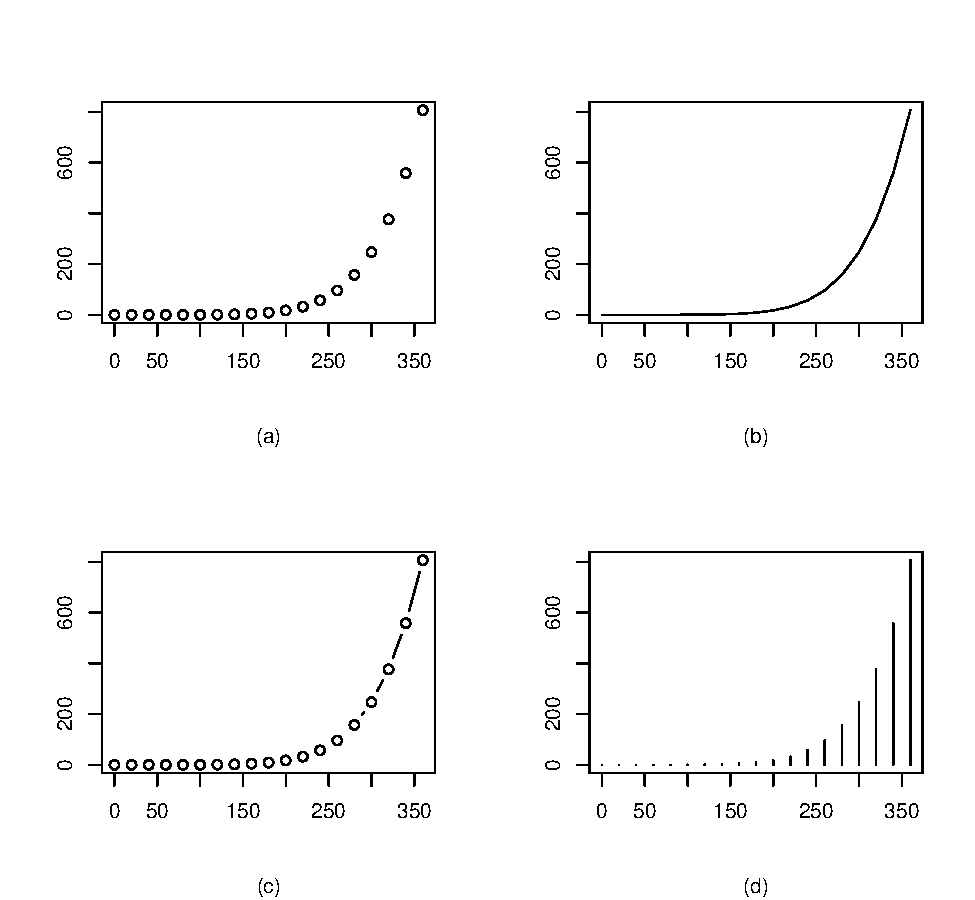
\includegraphics[width=0.8\linewidth]{BP_files/figure-latex/graf_typy-1} 

}

\caption{\label{fig1} Porovnání základních typů grafů: (a) - bodový, (b) - liniový, (c) - složený, (d) - histogram}\label{fig:graf_typy}
\end{figure}

Popis a všechny atributy dalších parametrů funkce \texttt{plot()} lze
nalézt v nápovědě zadáním příkazu \texttt{?plot()}.

\hypertarget{distribution}{\subsubsection{2.3 Vykreslení rozdělení v
R}\label{distribution}}

\qquad Teorie pravděpodobnosti je základem statistiky a R má hodně
nástrojů pro práci s pravděpodobnosti, rozdělením pravděpodobnosti a
náhodnými proměnnými. R má zkrácený název pro každé rozdělení
pravděpodobnosti. {[}19{]} Tyto názvy slouží k~identifikaci funkcí
spojených s rozděleními. Například zkrácený název \enquote{norm} pro
normální rozdělení, \enquote{exp} pro exponenciální rozdělení a další.
Funkce pak mají formu:

\begin{table}[H]
\centering
\begin{tabular}{@{}ll@{}}
\toprule
Funkce & \multicolumn{1}{c}{Účel}                     \\ \midrule
dxxxx  & Hustota pravděpodobnosti                     \\
pxxxx  & Distribuční funkce                           \\
qxxxx  & Kvantilová funkce                            \\
rxxxx  & Generátor náhodných čísel z daného rozdělení \\ \bottomrule
\end{tabular}
\caption{Funkce pro práci s rozděleními}
\label{tab2}
\end{table}

Funkce v R lze vykreslovat pomocí funkce \texttt{curve()} z balíčku
\texttt{graphics}. Lze vykreslit jak standardní funkce, tak i funkce
definované uživatelem. Například hustotu pravděpodobnosti normálního
rozdělení a její distribuční funkci můžeme vykreslit tímto způsobem
(Obrázek \ref{fig2}):

\begin{Shaded}
\begin{Highlighting}[]
\KeywordTok{curve}\NormalTok{(}\KeywordTok{dnorm}\NormalTok{(x))}
\KeywordTok{curve}\NormalTok{(}\KeywordTok{pnorm}\NormalTok{(x))}
\end{Highlighting}
\end{Shaded}

\begin{figure}[H]

{\centering 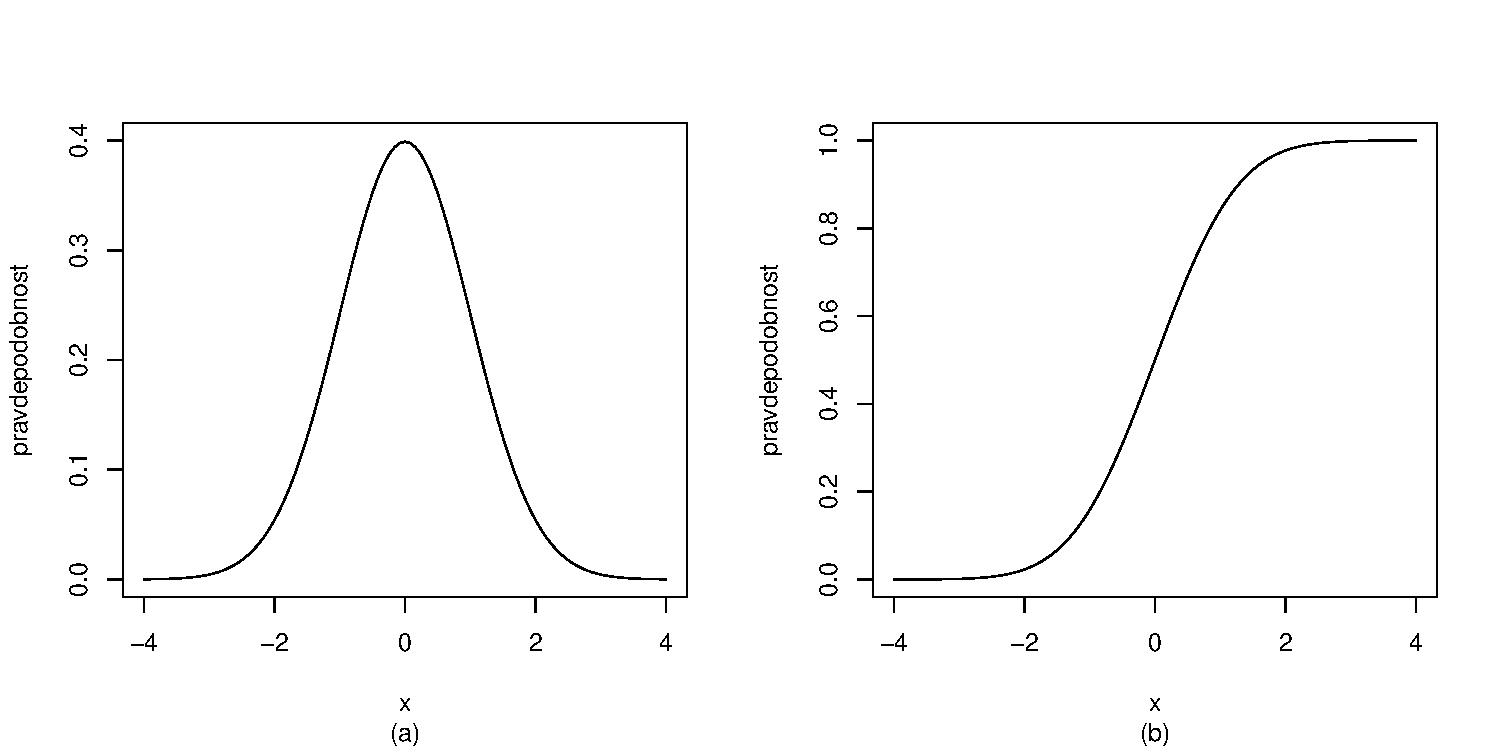
\includegraphics{BP_files/figure-latex/normal-1} 

}

\caption{\label{fig2} Hustota pravděpodobnosti normálního rozdělení (a) a její distribuční funkce (b)}\label{fig:normal}
\end{figure}

\newpage

\hypertarget{qqpp}{\paragraph{2.3.1 Q-Q graf a P-P graf}\label{qqpp}}

\qquad Q-Q (\emph{quantile-quantile}) graf a P-P
(\emph{probability--probability} nebo \emph{percent--percent}) graf
(Obrázek \ref{fig3}) se používají hlavně k testování normality při
průzkumové analýze dat \protect\hyperlink{normtests}{3.4}. Další způsob,
jak zjistit zda-li data mají normální rozdělení je sestrojení histogramu
(viz. sekce \protect\hyperlink{hist}{1.4.1}), avšak použití Q-Q grafu je
přesnější.

\qquad Princip Q-Q grafu spočívá v porovnání dvou rozdělení
pravděpodobnosti pomocí vykreslení jejich kvantilů proti sobě. Na jedné
ose se nacházejí teoretické kvantily normálního rozdělení a na druhé ose
kvantily naměřené (pozorované). Pokud data mají přesně normální
rozdělení, všechny body grafu leží na přímce 45°. Vztah hustoty
rozdělení a Q-Q grafu je znázorněn na obrázku \ref{fig12}. {[}19{]}
{[}10{]}

\qquad Princip P-P grafu je obdobný jako u Q-Q grafu: vykreslují se dvě
distribuční funkcí proti sobě (jedná teoretická a jedná pozorovaná) a
pokud všechny body grafu leží přibližně na přímce, jedná se o normální
rozdělení. Z velké části se P-P graf používá k vyhodnocení koeficientu
šikmosti rozdělení.{[}21{]}

V R se Q-Q graf vykreslí takto:

\begin{Shaded}
\begin{Highlighting}[]
\KeywordTok{qqnorm}\NormalTok{(x)}
\KeywordTok{qqline}\NormalTok{(x)}
\end{Highlighting}
\end{Shaded}

P-P graf v R lze vykreslit například následovně:

\begin{Shaded}
\begin{Highlighting}[]
\KeywordTok{plot}\NormalTok{(}\KeywordTok{ppoints}\NormalTok{(}\KeywordTok{length}\NormalTok{(x)), }\KeywordTok{sort}\NormalTok{(}\KeywordTok{pnorm}\NormalTok{(x)))}
\KeywordTok{abline}\NormalTok{(}\DecValTok{0}\NormalTok{,}\DecValTok{1}\NormalTok{)}
\end{Highlighting}
\end{Shaded}

\begin{figure}[H]

{\centering 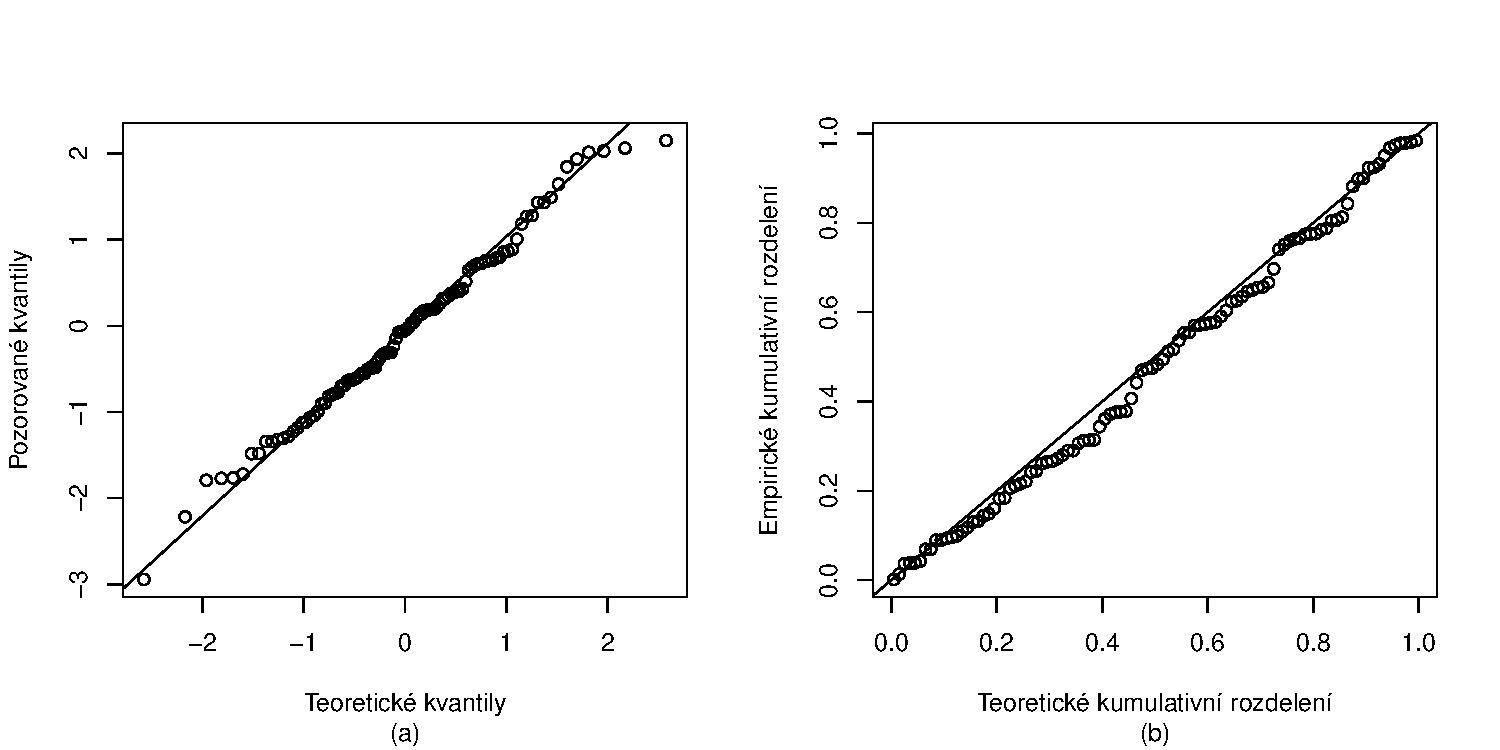
\includegraphics{BP_files/figure-latex/pp-qq plots-1} 

}

\caption{\label{fig3} Q-Q Graf (a) a P-P Graf (b)}\label{fig:pp-qq plots}
\end{figure}

\newpage

\hypertarget{boxplot}{\paragraph{2.3.2 Krabicový graf}\label{boxplot}}

\qquad Krabicový graf poskytuje rychlé a jednoduché vizuální shrnutí
datasetu. V základním prostředí R se vykreslí pomocí funkce
\texttt{boxplot()} z balíčku \texttt{graphics}. Obrázek \ref{fig4}
znázorňuje typický krabicový graf, kde silná čára je medián, krabice
kolem ní určuje polohu prvního a třetího kvartilů (dolní
Q\textsubscript{1} kvantil 25\% a horní Q\textsubscript{3} kvantil
75\%). ''Vousy`` (\emph{whiskers}) nad a pod krabici znázorňují rozpětí
dat bez odlehlých hodnot. Odlehlé hodnoty jsou definovaný jako hodnoty
ležící ve větší vzdálenosti od krabice než 1,5 \(\times\) IQR, kde IQR
je mezikvartilové rozpětí (\emph{interquartile range}) neboli
\(Q_3 - Q_1\).

\begin{Shaded}
\begin{Highlighting}[]
\KeywordTok{boxplot}\NormalTok{(x)}
\end{Highlighting}
\end{Shaded}

\begin{figure}[H]

{\centering 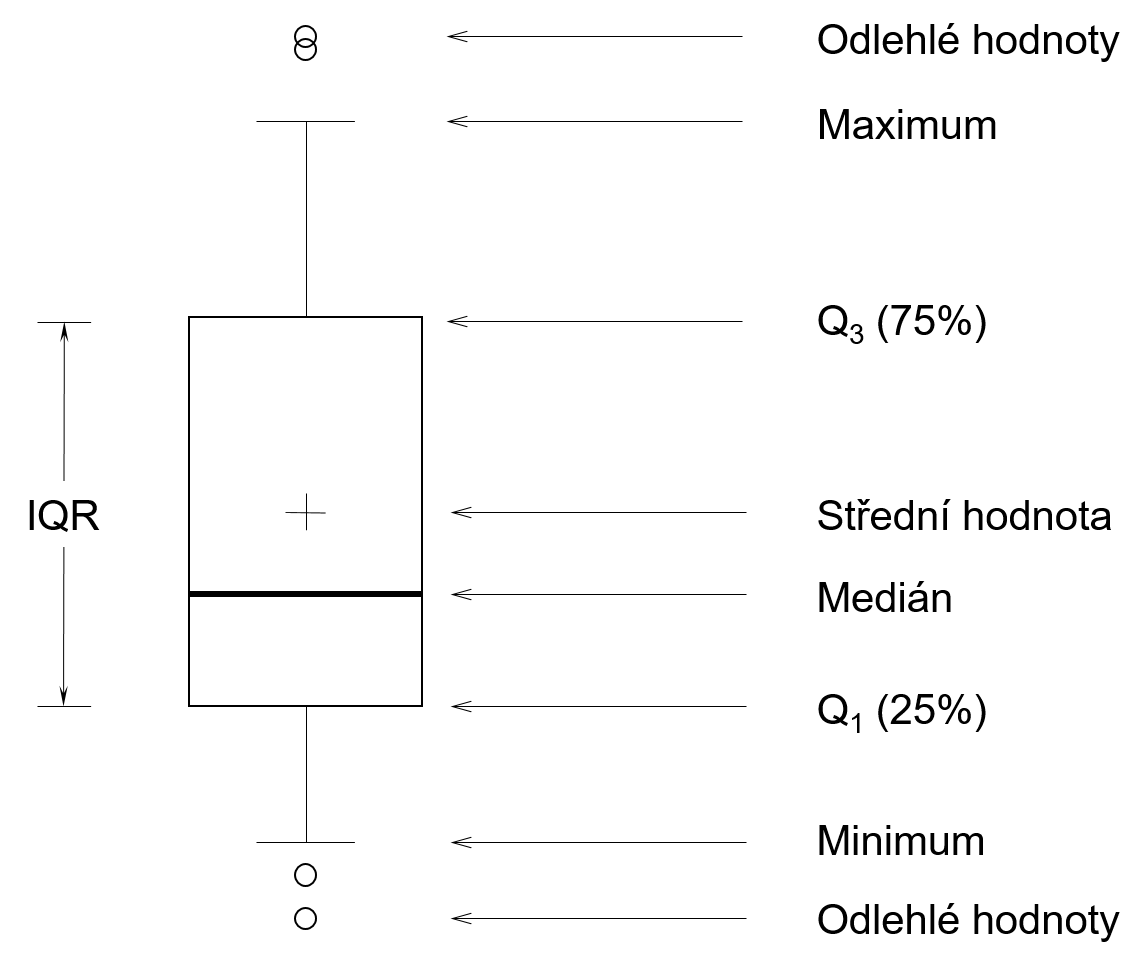
\includegraphics[width=0.65\linewidth]{fig/boxplot} 

}

\caption{\label{fig4} Boxplot}\label{fig:boxplot_img}
\end{figure}

\newpage

\subsubsection{2.4 Sloupcový graf}\label{sloupcovy-graf}

\qquad Sloupcový graf je jedním z nejvíce používaných způsobů
vizualizace dat. Obvykle se používá pro zobrazení kvantitativních hodnot
na ose y a kvalitativních na ose x. Výška sloupců může reprezentovat jak
četnosti výskytu hodnot, tak i samotné hodnoty.{[}22{]}

\qquad V R lze tento typ grafu vykreslit pomocí funkce
\texttt{barplot()}. V příkladu (Obrázek \ref{fig5}) je použit data set
\texttt{mtcars}, konkretně atribut \texttt{cyl} - počet válců v motoru.

\begin{Shaded}
\begin{Highlighting}[]
\KeywordTok{table}\NormalTok{(mtcars}\OperatorTok{$}\NormalTok{cyl)}
\end{Highlighting}
\end{Shaded}

\begin{verbatim}
## 
##  4  6  8 
## 11  7 14
\end{verbatim}

\begin{Shaded}
\begin{Highlighting}[]
\KeywordTok{barplot}\NormalTok{(}\KeywordTok{table}\NormalTok{(mtcars}\OperatorTok{$}\NormalTok{cyl))}
\end{Highlighting}
\end{Shaded}

\begin{figure}[H]

{\centering 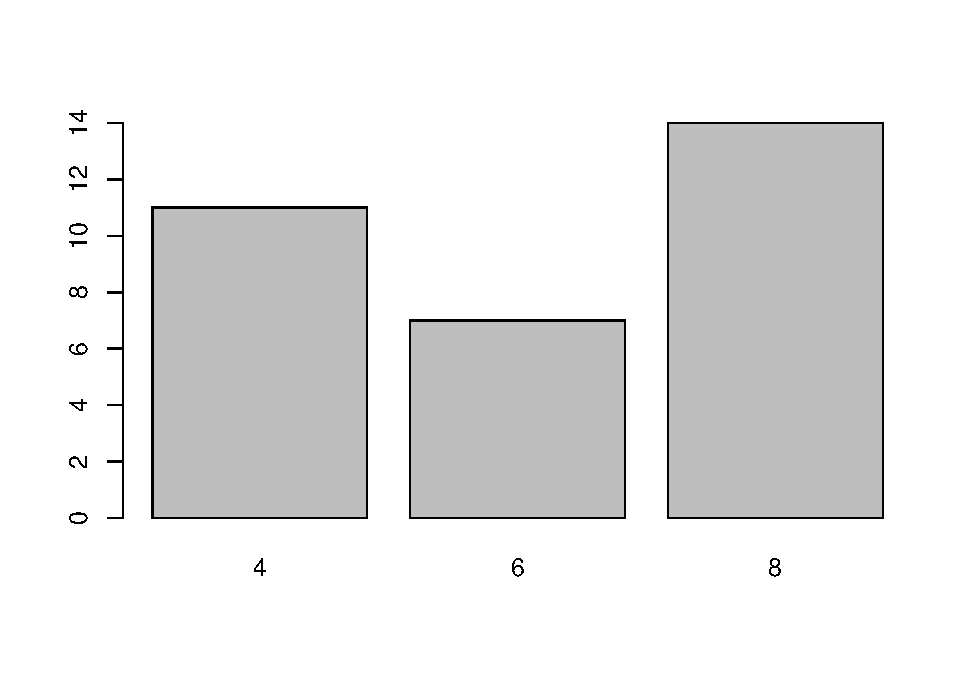
\includegraphics[width=0.55\linewidth]{BP_files/figure-latex/barplot-1} 

}

\caption{\label{fig5} Ukázka jednoduchého sloupcového grafu}\label{fig:barplot}
\end{figure}

\hypertarget{hist}{\subsubsection{2.4.1 Histogram}\label{hist}}

\qquad Sloupcový graf s četnostmi na souvislé ose je taky známý jako
histogram.{[}22{]} Četnosti mohou být absolutní či relativní. Absolutní
četnost zobrazuje počet statistických jednotek s hodnotou znaku, který
patří do určitého intervalu. Podíl příslušné četnosti a rozsahu datového
souboru se nazývá relativní četnost.{[}23{]} Šířka sloupce reprezentuje
jednotlivé intervaly, které mají stejnou délku. Pro výpočet optimální
délky intervalu existují různé metody. Základní histogram se vytváří
pomocí funkci \texttt{hist()} a její atribut \texttt{breaks} udává buď
hranice intervalů, jejich preferovaný počet nebo metodu výpočtu
intervalu. V R jsou vestavěny 3 metody výpočtu:

\newpage

\begin{enumerate}
\def\labelenumi{\arabic{enumi}.}
\tightlist
\item
  Sturges {[}24{]}
\end{enumerate}

\begin{Shaded}
\begin{Highlighting}[]
\KeywordTok{hist}\NormalTok{(x, }\DataTypeTok{breaks =} \StringTok{"Sturges"}\NormalTok{)}
\end{Highlighting}
\end{Shaded}

\[k=[log_2(n)]+1\] Kde \(k\) je počet intervalů a \(n\) je počet prvků
neboli počet pozorování výběru \(x\). Tato metoda je výchozí pro funkci
\texttt{hist()}.

\begin{enumerate}
\def\labelenumi{\arabic{enumi}.}
\setcounter{enumi}{1}
\tightlist
\item
  Scott {[}24{]}
\end{enumerate}

\begin{Shaded}
\begin{Highlighting}[]
\KeywordTok{hist}\NormalTok{(x, }\DataTypeTok{breaks =} \StringTok{"Scott"}\NormalTok{)}
\end{Highlighting}
\end{Shaded}

Scotovo pravidlo je následující:
\[h=\frac{3.5 \sigma}{n^{\frac{1}{3}}}\] kde \(\sigma\) je směrodatná
odchylka a \(h\) je předpokládaná šířka intervalu.

Počet intervalů může být vypočítán pomocí vztahu:
\[k=\Big[\frac{max(x)-min(x)}{h}\Big]\]

Případně oba vztahy lze shrnout do jednoho:
\[k = \Big[n^{\frac{1}{3}}{\frac{max(x)-min(x)}{3.5 \sigma}}\Big]\]

\begin{enumerate}
\def\labelenumi{\arabic{enumi}.}
\setcounter{enumi}{2}
\tightlist
\item
  Freedman--Diaconis {[}25{]}
\end{enumerate}

\begin{Shaded}
\begin{Highlighting}[]
\KeywordTok{hist}\NormalTok{(x, }\DataTypeTok{breaks =} \StringTok{"FD"}\NormalTok{)}
\end{Highlighting}
\end{Shaded}

Freedman--Diaconisovo pravidlo pro stanovení předpokládané šířky
intervalu je:

\[h=2\frac{IQR(x)}{n^{\frac{1}{3}}}\] Po dosazení:
\[k = \Big[n^{\frac{1}{3}}{\frac{max(x)-min(x)}{2IQR(x)}}\Big]\]

kde \(IQR\) je mezikvartilové rozpětí, které definujeme jako rozdíl
třetího a prvního kvartilů.

Histogram je jedním ze standardních způsobů, používaných k odhadu tvaru
rozdělení, přesto se ale tento způsob považuje za nepřesný, vzhledem k
ovlivnění tvaru počtem použitých intervalů. Při normálním rozdělení by
měl histogram mít zvoncovitý tvar schodný s Gaussovou křivkou (Obrázek
\ref{fig6}).

\begin{figure}[H]

{\centering 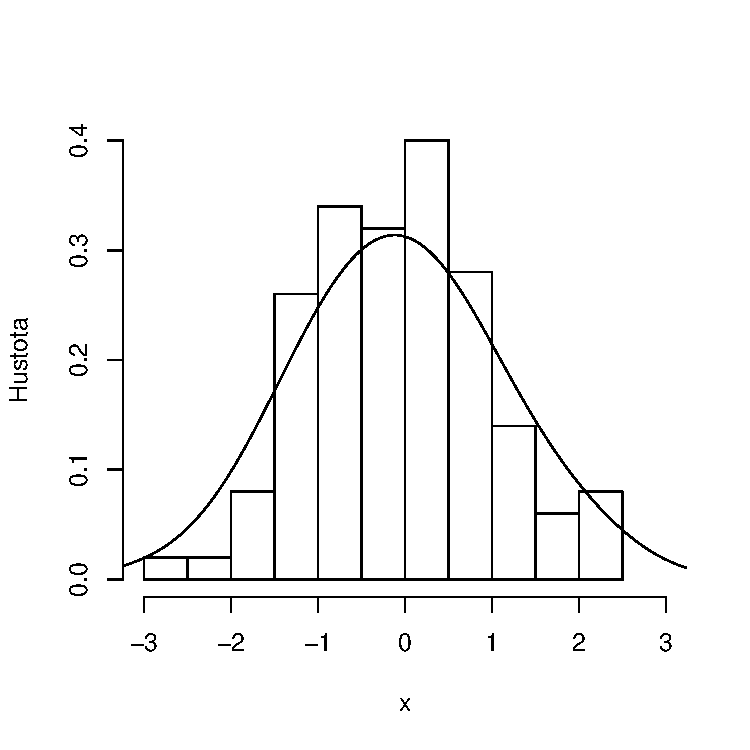
\includegraphics[width=0.6\linewidth]{BP_files/figure-latex/hist_example-1} 

}

\caption{\label{fig6} Histogram s odhadem hustoty pravděpodobnosti}\label{fig:hist_example}
\end{figure}

\paragraph{2.4.2 Koláčový graf}\label{kolacovy-graf}

\qquad Koláčový graf představuje plný kruh (360°), který je rozdělen na
jednotlivé výseče pro znázornění číselných proporci mezi proměnnými.
Koláčový graf je tvořen transformaci skládaného sloupcového grafu do
polárního souřadnicového systému (Obrázek \ref{fig7}). {[}12{]}

\begin{figure}[H]

{\centering 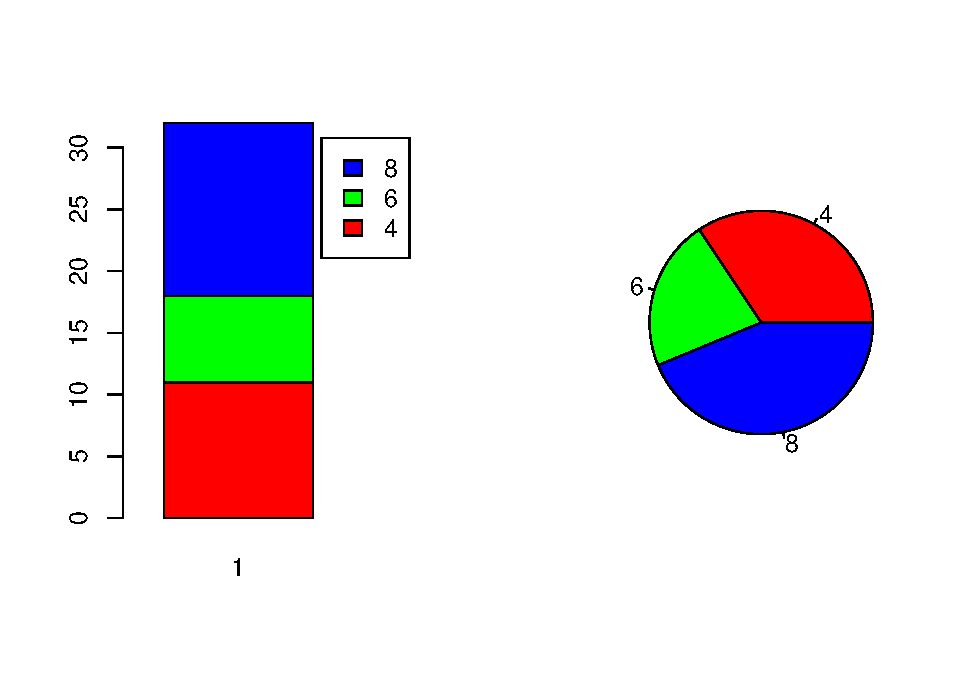
\includegraphics[width=0.65\linewidth]{BP_files/figure-latex/barplot_to_pie-1} 

}

\caption{\label{fig7} Skládaný sloupcový graf transformovaný do polárního souřadnicového systému}\label{fig:barplot_to_pie}
\end{figure}

\qquad Jednoduché koláčové grafy se vykreslují pomoci funkci
\texttt{pie()} (Obrázek \ref{fig8}).

\begin{figure}[H]

{\centering 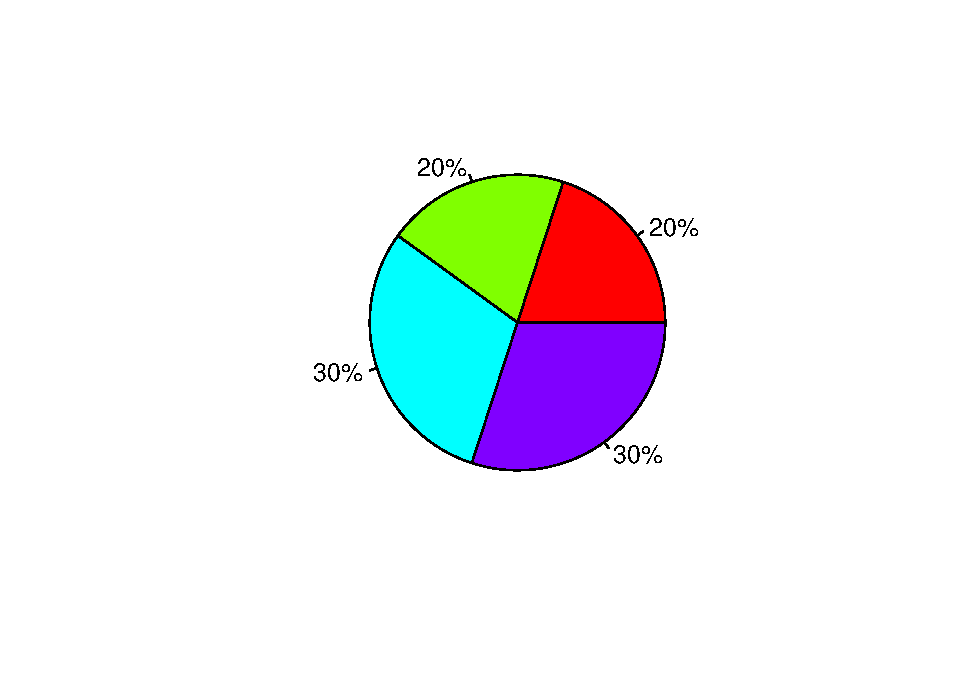
\includegraphics[width=0.65\linewidth]{BP_files/figure-latex/pie_example-1} 

}

\caption{\label{fig8} Ukázka jednoduchého koláčového grafu}\label{fig:pie_example}
\end{figure}

\hypertarget{stem-and-leaf}{\paragraph{\texorpdfstring{2.4.3 Číslicový
histogram
(\emph{stem-and-leaf})}{2.4.3 Číslicový histogram (stem-and-leaf)}}\label{stem-and-leaf}}

\qquad Číslicový histogram, jinak známy jako \emph{stem-and-leaf plot},
podobně jako histogram pomáhá vizualizovat tvar rozdělení. Jedná se
spíše o historický typ grafu, který byl populární v osmdesátých letech,
kvůli obtížnějšímu vykreslování velkých datasetu. Vstupní údaje jsou
rozdělené vertikální linií na dva sloupce. Pravý sloupec obsahuje listy
(\emph{leaf})~-~poslední číslice po desetinné čárce a levý sloupec
obsahuje stonek (\emph{stem})~-~číslice před desetinnou čárkou. Každý
stonek je uveden pouze jednou i pokud neobsahuje žádné listy. Listy se
uvádějí od nejmenšího po největší. {[}4{]} Proto v příkladu uvedeném
níže je v prvním řádku stonkem číslice -2 a listy jsou číslice 9 a 2.
Víme tak, že v datasetu se vyskytli čísla -2.9 a -2.2. Tento typ grafu v
prostředí R se vykresluje pomoci funkce \texttt{stem()}:

\begin{Shaded}
\begin{Highlighting}[]
\KeywordTok{stem}\NormalTok{(x)}
\end{Highlighting}
\end{Shaded}

\begin{verbatim}
## 
##   The decimal point is at the |
## 
##   -2 | 92
##   -1 | 888755333332211100
##   -0 | 99888877666666655554433332111100
##    0 | 0011122222233334444456777788888999
##    1 | 0233445689
##    2 | 0012
\end{verbatim}

\newpage

\hypertarget{EDA}{\subsection{3 Průzkumová analýza dat}\label{EDA}}

\begin{figure}[H]

{\centering 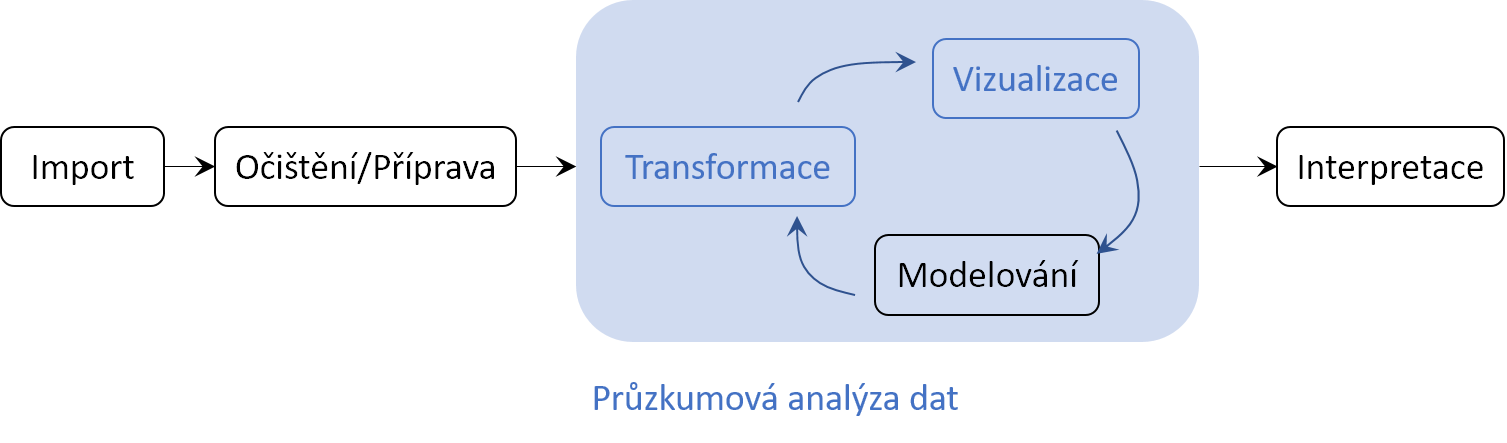
\includegraphics[width=1\linewidth]{fig/EDA_diagram2} 

}

\caption{\label{fig9} Posloupnost datové analýzy}\label{fig:diagram_img}
\end{figure}

\qquad Úkolem průzkumové analýzy dat (\emph{Explanatory Data Analysis},
zkráceně EDA) je vizualizace a transformace dat systematickým způsobem
za účelem maximálního pochopení dat, určení vztahu mezi nimi a posouzení
jejích kvality. EDA je důležitou části datové analýzy a měla by být
jedním z jejích prvních kroků.

\qquad Zařazení průzkumové analýzy dat do procesu datové analýzy je
zobrazeno v diagramu \ref{fig9}. Prvním krokem datové analýzy je
\textbf{import} dat. Obecně to v tomto případě znamená nahrání
obdržených dat ze souboru či databáze do prostředí R. Bez tohoto kroku
datová analýza nemůže být vykonána. V momentě když data jsou importována
do R je vhodné je \textbf{očístit} neboli \textbf{přípravit}. Tím je
myšleno ukládání dat v konzistentní a systematické formě, odpovídající
sémantice původního datasetu. Zkrátka očištěná data jsou taková data, ve
kterých sloupce odpovídají proměnným a řádky odpovídají pozorováním.
Takováto příprava dat usnadňuje další práci s nimi.

\qquad Jakmile jsou data očištěna, je obvyklým krokem jejich
\textbf{transformace}. Transformací se rozumí omezení pozorování
(například dle zájmového území či povodí), vytváření nových proměnných
na základě již existujících, agregace (např. z denního do měsíčního
kroku), výpočet souhrnných statistik (středních hodnot, kvantilů atd.),
odstranění odlehlých pozorování a normalizace. Poté, co jsou data
očištěná a obsahují veškeré potřebné proměnné, je možné na ně aplikovat
dva nejdůležitější nástroje k zjištění informací: vizualizaci a
modelování. Jakákoliv analýza tyto nástroje opakovaně využívá, ačkoliv
samozřejmě mají své výhody a nevýhody.

\qquad \textbf{Vizualizace} je schopná odhalit neočekávané chování dat a
napovědět další směr analýzy. Vizualizaci lze odhalit nevhodně zvolená
či špatně připravená data a nekorektní dotazování. I přesto, že
vizualizace je dobrým nástrojem datové analýzy, její aplikace na větší
datasety je značně náročná a interpretace výsledků je subjektivní, tudíž
závisí na analytikovi.

\qquad \textbf{Modelování} je v ramci průzkumové analýzy dat doplňkem
vizualizace. Jedná se o zásadně matematický a výpočetní nástroj, který
se obecně hodí i na větší datasety. Téměř každý model musí splňovat své
předpoklady, které by měli být ověřeny před jejich aplikací, na rozdíl
od vizualizace, která žádné předpoklady nevyžaduje.{[}26{]}

\qquad Důležitou součástí analýzy je \textbf{interpretace} výsledků a
formulace závěrů. Vyhodnocuje, jak dobře zvolený model či vizualizace
slouží k pochopení dat a jejich popisu. Je také důležité si uvědomit
komu jsou výsledky interpretovány, kdo je cílová skupina. Dobře
provedené grafické výstupy podložené jejich správnou interpretaci jsou
jedním z nejlepších způsobů prezentace dat.

\qquad Průzkumová analýza dat není specifikována jako konkrétní soubor
pravidel a postupů, ale jako přístup k analýze dat. Obvykle zahrnuje
následující kroky:

\begin{itemize}
\tightlist
\item
  Vyhledávání vybočujících (odlehlých) pozorování
\item
  Náhrada chybějících hodnot
\item
  Transformace dat
\item
  Změny typu proměnných
\item
  Ověřování normality
\end{itemize}

\subsubsection{3.1 Odlehlá pozorování}\label{odlehla-pozorovani}

\qquad Odlehlá pozorování (\emph{outliers}) jsou významně odlišná vůči
ostatním hodnotám datasetu. Definice toho, jak moc odlišná taková
pozorování mají být je dáno analytikem na základě konkretního datasetu a
kontextu problematiky. Tato pozorování mohou být indikátorem chybných
dat nebo vzácných událostí. Důvody proč se tato pozorování vyskytují by
měli být pečlivě zkoumány. Dále je důležité posoudit, jak je jimi
výsledek analýzy ovlivněn, případně zdali je předpoklady metody
připouštějí.

\qquad Hledání odlehlých, vybočujících, pozorování a jiných anomálií pro
jednotlivé veličiny lze provést graficky například pomoci boxplotu (viz.
sekce \protect\hyperlink{boxplot}{2.3.2}), bodových grafů
(\protect\hyperlink{scatterplot}{2.1}) nebo číslicových histogramů
(\protect\hyperlink{stem-and-leaf}{2.4.3}). Dají se také vypočítat
pomocí různých statistik, například metodou \emph{jackknife}, která je
popsána v následující kapitole (\protect\hyperlink{jackknife}{3.1.1}). V
momentech, kdy je vizualizace obtížná (velké datasety, větší množství
navzájem se ovlivňujících proměnných, atd.), využívají se nástroje
vícerozměrné, například Mahalanobisovy vzdálenosti
(\protect\hyperlink{mbdist}{3.1.2}), \emph{leverages}
(\protect\hyperlink{leverages}{3.1.3}) a další.

\hypertarget{jackknife}{\paragraph{\texorpdfstring{3.1.1
\emph{Jackknife}}{3.1.1 Jackknife}}\label{jackknife}}

\qquad Metoda byla původně představená Johnem W. Tukey v roce 1958 v
\enquote{\emph{The Annals of Mathematical Statistic}} {[}27{]} a jedná
se o speciální případ metody \emph{bootstrap} (více o metodě B. Efron a
R. Tibshirani v \enquote{\emph{An Introduction to the Bootstrap}}
{[}28{]}).

\qquad Postup metody \emph{jackknife} je založen na celkem jednoduché
myšlence. Zjišťují se souhrnné statistiky podsouborů (\emph{Jackknife
Samples}), které se vytvářejí postupným vypouštěním jednotlivých
pozorování z původního datasetu. Jinými slovy existuje \(n\) unikátních
Jackknife podsouborů a \(i\)-tý Jackknife podsoubor je definován jako
vektor.

\qquad Pomocí porovnání souhrnných statistik původního datasetu a
vytvořených Jackknife podsouborů se odhadne vliv jednotlivých pozorování
na původní dataset. Jedná ze souhrnných statistik, kterou lze použít je
střední hodnota \(\bar{x}\). Pro původní dataset obsahující \(n\)
pozorování lze střední hodnotu odhadnout dle vzorce
\(\bar{x} = \frac{1}{n} \sum \limits_{i=1}^{n} \bar{x}_i\). Střední
hodnota Jackknife podsouborů se vyhodnotí následovně:
\[\bar{x}_i = \frac{1}{n-1} \sum \limits_{j=1, j \neq i}^{n} x_j, \quad \text{kde } i=1,\dots,n.\]
Porovnání lze provést dle vzorce
\(\textit{Var}(\bar{x}) = \frac{n-1}{n} \sum \limits_{i=1}^{n}(\bar{x}_i - \bar{x})^2\),
kde \(\textit{Var}(\bar{x})\) je odhad rozptylu, který indikuje, jak moc
jednotlivá pozorování ovlivňují dataset, tj. přítomnost odlehlých
pozorování. Metoda může být také použita k odhadu skutečné, neovlivněné
střední hodnoty datasetu. {[}29{]}

\hypertarget{mbdist}{\paragraph{3.1.2 Mahalanobisovy
vzdálenosti}\label{mbdist}}

\qquad K měření vzdálenosti mezi objekty se často používá euklidovská
vzdálenost. Euklidovská vzdálenost je jednoduchá na výpočet a
interpretaci, ale není schopná brát v úvahu vztahy mezi daty. Proto je v
řádě případů vhodné použít mahalanobisovou vzdálenost. Je definovaná
matice \(\bm{X}(n \times p)\), obsahující \(n\) objektů \(\bm{x}_i\) a
\(p\) proměnných. Euklidovská vzdálenost mezi vektorem \(i\)-tého řádku
\(\bm{x}_i (1 \times p)\) této matice a vektoru středních hodnot
\(\bar{\bm{x}} (1 \times p)\) se spočítá jako
\[ED_i = \sqrt{(\bm{x}_i - \bar{\bm{x}})(\bm{x}_i - \bar{\bm{x}})^T}, \quad \text{pro } i = 1,\dots,n\]
zatímco mahalanobisova vzdálenost se spočítá jako
\[MD_i = \sqrt{(\bm{x}_i - \bar{\bm{x}}) \bm{C}^{-1}_x (\bm{x}_i - \bar{\bm{x}})^T}, \quad \text{pro } i = 1,\dots,n\]
kde \(\bm{C}_x\) je kovarianční matice. {[}30{]}

\qquad Na obrázku \ref{fig10} jsou znázorněny elipsy mahalanobisových
vzdáleností, kde každá elipsa představuje vzdálenost od průměru. Z
tohoto je zřejmé, že vzdálenost roste pomaleji ve směru korelace.
Pozorování, které je výrazně vzdáleno od středu, ale leží ve směru
závislosti, má nižší mahalanobisovou vzdálenost než pozorování, které je
stejně vzdáleno od středu, ale neleží ve směru závislosti. Tato
vlastnost mahalanobisových vzdálenosti umožňuje identifikaci odlehlých
pozorování.

\qquad Metoda byla představena P.C. Mahalanobisem v roce 1936 ve článku
\emph{\enquote{On the Generalized Distance in Statistics}} {[}31{]}.
Mahalanobisové vzdálenosti se používají nejenom k nalezení odlehlých
pozorování, ale i ke zkoumání reprezentativity mezi dvěma data sety,
aplikuje se v algoritmu \(k\)-nejbližších sousedů, v diskriminační
analýze a má mnoho dalších uplatnění.

\begin{figure}[H]

{\centering 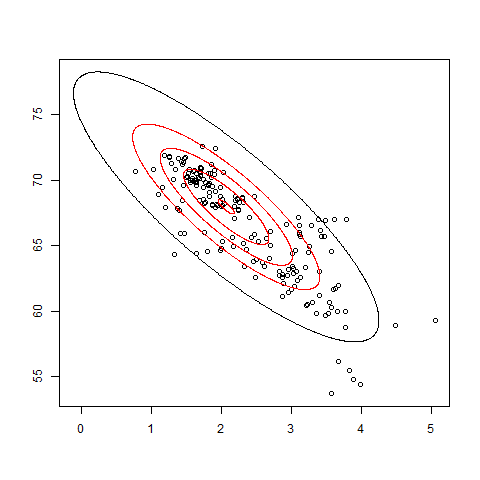
\includegraphics[width=0.65\linewidth]{fig/mahalanobis} 

}

\caption{\label{fig10} Mahalanobisovy vzdálenosti}\label{fig:mbdist_img}
\end{figure}

\hypertarget{leverages}{\paragraph{3.1.3 Leverages}\label{leverages}}

\qquad Leverage (případně též efekt, vliv nebo projekční \(h\) prvek) se
používá v regresní analýze k měření velikosti vlivu pozorování na
regresní odhad. Princip metody spočívá v kontrole diagonálních prvků
projekční matice \(\bm{H}\), která je produktem metody nejmenších
čtverců a je definována
\[\bm{H} = \bm{X}(\bm{X}^T\bm{X})^{-1}\bm{X}^T.\] Model lineární regrese
může být zapsán následovně:
\[\bm{y} = \bm{X \beta} + \bm{\varepsilon},\] kde vektor vysvětlované
proměnné je \(\bm{y}\), matice vysvětlujících proměnných je \(\bm{X}\),
vektor regresních koeficientů, který je odhadován, je \(\bm{\beta}\) a
vektor náhodné složky je \(\bm{\varepsilon}\). Metoda nejmenších čtverců
poskytuje řešení regresních rovnic:
\[\bm{\beta} = (\bm{X}^T\bm{X})^{-1} \bm{X}^T \bm{y}.\] Lze dosadit:
\[\hat{\bm{y}} = \bm{X \beta} = \bm{X}(\bm{X}^T\bm{X})^{-1} \bm{X}^T \bm{y}.\]
Výsledný vektor má tvar \(\hat{\bm{y}} = \bm{Hy}\), kde \(\bm{H}\) je
projekční matice. {[}32{]}

\subsubsection{3.2 Náhrada chybějících
pozorování}\label{nahrada-chybejicich-pozorovani}

\qquad Problém chybějících pozorování spočívá v neschopnosti jejich
zpracovávání některými metodami. Takové hodnoty lze vynechat nebo
doplnit (nahradit) jednou z řady metod. Vynechání hodnot vede k
nežádoucímu zmenšení datasetu, proto je výhodnější chybějící údaje
doplnit. Nejednodušším nástrojem pro náhradu chybějících hodnot je
aritmetický průměr příslušné proměnné. Tento způsob může vést ke
zkresleným odhadům (neplatí-li předpoklad, že chybějící údaje jsou zcela
náhodné) a podhodnocuje variabilitu a kovarianci datasetu, a proto se
nedoporučuje v případě vyššího podílu chybějících údajů. Další možnou
metodou je náhrada náhodným číslem generovaným z příslušného rozdělení
(parametry jsou odhaduty z výběru). V tomto případě se respektuje
variabilita datasetu, ale nerespektuje se jeho kovariance. Chybějící
údaje lze také odvodit pomocí známých hodnot na základě pomocné
jednoduché lineární regresní funkce. Tato metoda respektuje nejenom
variabilitu vzorku, ale i jeho korelační strukturu. {[}33{]}

\subsubsection{3.3 Transformace dat}\label{transformace-dat}

\qquad Jedním z cílů transformace dat je dosažení srovnatelnosti
proměnných: sjednocení měřítka, variace a typu proměnných. Hlavním
využitím je splnění podmínek vyžadovaných metodami, například podmínky
normality, kde je snaha převést data na normální rozdělení, snížení
vlivu rušivých proměnných (odlehlých hodnot) atd. {[}34{]} Rozdělujeme
transformaci lineární (centrování, normování) a nelineární (plynoucí z
typu a charakteru dat).

\qquad Lineární transformace zachovává lineární vztahy mezi proměnnými.
Jedním z příkladů takovéto úpravy dat je metoda centrování, která se
používá u vícerozměrných analýz. Podstata metody spočívá v zachování
měřítka vzorku při změně hodnot: od původních hodnot se odečítá průměr
proměnné (od prvků sloupce se odečte jejich sloupcový průměr), průměry
získaných nových proměnných se tudíž rovnají nule. Toto lze zapsat
následovně: \[v_{ij} = x_{ij} - \bar{x}_j\] Vektor průměrů
\(\bar{\bm{v}}\) je nulový, kovariance a korelace proměnných zůstává
nezměněna. {[}35{]} Další často využívanou metodou je metoda normalizace
dat. Tato metoda transformuje měřítka vzorků pro možnost jejich
porovnání (eliminuje jednotky měření), po úpravě střední hodnota vzorku
tedy odpovídá nule a odchylka jedničce (normální rozdělení).
\[z_{ij} = \frac{x_{ij} - \bar{x}_j}{\sigma(x_j)}\] \(\sigma(x_j)\) je
směrodatná odchylka sloupce proměnné, vektor průměrů \(\bar{\bm{z}}\) je
nulový a kovariance vektoru nových proměnných se shoduje s korelací
původního vektoru. {[}36{]}

\qquad Nelineární transformace vyplývá z typu dat a mění (snižuje či
zvyšuje) lineární vztahy mezi proměnnými a to znamená, že nezachovává
korelaci mezi nimi. Pokud data mají charakter absolutní četnosti,
používá se odmocninová transformace \(X^{\prime} = \sqrt{X}\), pokud
odpovídají log-normálnímu rozdělení, používá se logaritmická
transformace \(X^{\prime} = \log_{10}X\) atd. Logaritmus náhodné
veličiny s log-normálním rozdělením má normální rozdělení (viz obrázek
\ref{fig11}). Logaritmická transformace může být použita pouze u
nezáporných rozdělení. {[}37{]} {[}38{]}

\begin{figure}[H]

{\centering \includegraphics[width=0.82\linewidth]{BP_files/figure-latex/lognormal_to_normal-1} 

}

\caption{\label{fig11} Log-normální rozdělení transformováné na normální rozdělení}\label{fig:lognormal_to_normal}
\end{figure}

\hypertarget{normtests}{\subsubsection{3.4 Ověřování
normality}\label{normtests}}

\qquad Důležitým aspektem popisu proměnné je tvar jejího rozdělení,
který udává četnosti hodnot z různých rozsahů proměnné. Většina
statistických testů a metod se zakládá na předpokladu, že proměnná má
normální rozdělení. Z tohoto důvodu je vhodné ověřovat normalitu
rozdělení analyzovaného vzorku.

\qquad Zjistit zda-li vzorek pochází z normálního rozdělení lze
grafickým posouzením nebo pomocí testů normality. Mezi nástroje
grafického posouzení normality se řadí histogram rozdělení četnosti
(kapitola \protect\hyperlink{hist}{2.4.1}), graf výběrové distribuční
funkce (\protect\hyperlink{distribution}{2.3}), Q-Q graf a P-P graf
(\protect\hyperlink{qqpp}{2.3.1}). Vztah hustoty rozdělení a Q-Q grafu
je znázorněn na obrázku \ref{fig12}. Dále existuje řada testů normality,
zde jsou popsany testy Shapiro-Wilk (SW) a Jarqua-Bera (JB).

\begin{figure}[H]

{\centering \includegraphics[width=0.95\linewidth]{BP_files/figure-latex/density_qq_plot-1} 

}

\caption{\label{fig12} Vztah hustoty rozdělení a Q-Q grafu pro různá narušení normality}\label{fig:density_qq_plot}
\end{figure}

\qquad Shapiro-Wilk test byl poprvé představen v roce 1965 S. S.
Shapirem a M. Wilkem {[}39{]}. Metoda dokáže pracovat se vzorky
velikosti 12 až 5000 pozorování. Nulová hypotéza tohoto testu
předpokládá, že vzorek má normální rozdělení. Pokud \(p\)-hodnota je
menší, než zvolená hladina významnosti, zamítá se nulová hypotéza,
jinými slovy vzorek nemá normální rozdělení. Statistika testu vypadá
následovně:
\[W = \frac{\big(\sum \limits^n_{i=1} a_i x_{(i)}\big)^2}{\sum \limits^n_{i=1}(x_i - \bar{x})^2},\]
kde \(x_{(i)}\) je \(i\)-tý nejmenší prvek (statistika \(i\)-tého řádu),
\(\bar{x}\) je průměr vzorku, \(n\) je počet pozorování.

\qquad Jarqua-Bera test závisí na koeficientech šikmosti a špičatosti.
Statistika JB testu může být zapsána:
\[T = n \bigg( \frac{(\sqrt{b_1})^2}{6} + \frac{(b_2 - 3)^2}{24} \bigg),\]
kde \(n\) je velikost vzorku, \(\sqrt{b_1}\) je koeficient šikmosti
vzorku a \(b_2\) je koeficient špičatosti. Nulová a alternativní
hypotéza se schoduje s SW testem. Používá se pro větší datasety nad 2000
pozorování. {[}40{]} \newpage

\subsection{4 Pokročilá vizualizace v
R}\label{pokrocila-vizualizace-v-r}

\hypertarget{base}{\subsubsection{4.1 Balíčky pro vizualizaci
dat}\label{base}}

\qquad Vestavený balíček \texttt{base} byl vyvinut Rossem Ihaka na
základě zkušeností s implementací grafických ovladačů do S (předchůdce
R). Grafy v \texttt{base} mají charakter grafů na papíře: stávající
obsah nelze modifikovat ani odstranit. Do grafu lze přidávat potřebné
prvky, které jsou vykreslovány na povrch grafu a po vykreslení nemohou
být dále měněny. V \texttt{base} neexistuje jiná uživateli přístupná
reprezentace, než ta, co se objeví na obrazovce. \texttt{base} obsahuje
nástroje pro kreslení jak primitivních, tak i kompletních výkresů.
Funkce tohoto balíčku jsou obecně rychlé, ale mají omezené možnosti.
Vykreslení základních grafů v R je popsáno v kapitole
\protect\hyperlink{base}{2}.

\qquad Mimo \texttt{base} má uživatel možnost využít rozsáhlou nabídku
dalších balíčků. Následující kapitoly obsahují kratký popis vybraných
balíčku (\texttt{grid}, \texttt{lattice}, \texttt{ggplot2}). V R
existuje mnoho dalších balíčků, například \texttt{vcd}, \texttt{plotrix}
a \texttt{gplot}, které implementují speciální grafiku, avšak žádný z
nich neposkytuje rámec pro tvorbu statistických grafů. Pro instalaci
balíčků se používá příkaz \texttt{install.packages()}. Komplexní zdroj,
úvádějící všechny grafické funkce dostupné v ostatních balíčcích
vyvinutých komunitou lze nalézt na stránce
\url{http://cran.r-project.org/web/views/Graphics.html}. {[}12{]}

\paragraph{\texorpdfstring{4.1.1 \texttt{grid}}{4.1.1 grid}}\label{grid}

\qquad \texttt{grid} je alternativou jednoduché grafiky z \texttt{base}
s rozsáhlejšími možnosti pro úprávu grafu. Vývoj balíčku začal v roce
2000. Autorem je Paul Murrell a balíček vznikl na základě jeho doktorské
práce \emph{Investigations in Graphical Statistics} z roku 1998
{[}41{]}. Grafické objekty v \texttt{grid} mohou být reprezentovány
nezávislé na grafu a později upraveny. Systém \emph{viewport}ů (každý
obsahuje vlastní souřadnicový systém) usnadňuje rozvržení komlexní
grafiky. Balíček umožňuje vykreslení jednotlivých výkresů, avšak nemá
nástroje pro tvorbu statistických grafů. {[}42{]}

\paragraph{\texorpdfstring{4.1.2
\texttt{lattice}}{4.1.2 lattice}}\label{lattice}

\qquad Deepayanem Sarkarem vyvinutý balíček \texttt{lattice} používá
grafiku \texttt{grid} k implementaci Clevelandového \emph{trellis}
grafického systému (viz kapitola \protect\hyperlink{cleveland}{1.2.2}),
což vedlo k značnému vylepšení grafiky oproti \texttt{base}. Pomocí
\texttt{lattice} lze jednoduše vykreslit \emph{trellis} graf a některé
detaily výkresu, jako například legenda, se vytváří automaticky. Avšak
\texttt{lattice} postrádá formální model, což může ztížit jeho
rozšíření. Tento balíček je dostačující pro typické grafické potřeby a
je dostatečně flexibilní i pro zvládnutí většiny nestandardních
požádavků.

\newpage

\hypertarget{ggplot}{\paragraph{\texorpdfstring{4.1.3
\texttt{ggplot2}}{4.1.3 ggplot2}}\label{ggplot}}

\qquad Balíček \texttt{ggplot2} byl vyvinut v roce 2005 Hadley Wickhamem
na základě \emph{The Grammar of Graphics} Lelanda Wilkinsona.
\texttt{ggplot2} přebírá přednosti balíčků \texttt{base} a
\texttt{lattice} a vylepšuje je silným základním modelem, který
podporuje tvorbu libovolného statistického grafu založeného na
principech popsaných v kapitole \protect\hyperlink{gg}{1.3}. Silný
základní model \texttt{ggplot2} umožňuje popsat širokou škálu grafiky
pomocí kompaktní syntaxe a nezávislé komponenty zjednodušují rozšíření.
Obdobně jako \texttt{lattice}, využívá \texttt{ggplot2} mřížky k
vykreslení grafiky, což znamená, že umožňuje úpravu vyhledu na mnohem
nižší úrovni.

\qquad Jako ukázku lze předvést graf vykreslený pomocí různých balíčků
(obrázky \ref{fig1a}, \ref{fig1b}, \ref{fig1c}). V představeném kódu
byly použity denní časové řady srážek z roku 2010 v oblasti povodí Labe
od pramene po Svatopetrský potok včetně. ID tohoto útvaru povrchových
vod je \texttt{HSL\_0010}. \texttt{DTM} odpovídá datumu v denním kroce a
\texttt{P} odpovídá úhrnu srážek v milimetrech. Každý balíček má
přednastavený počáteční vzhled, který lze úpravovat dle požádavků, avšak
pro tuto ukázku je nutno počáteční rozdíly naopak ponechat.

\begin{Shaded}
\begin{Highlighting}[]
\KeywordTok{plot}\NormalTok{(HSL_}\DecValTok{0010}\OperatorTok{$}\NormalTok{DTM, HSL_}\DecValTok{0010}\OperatorTok{$}\NormalTok{P, }\DataTypeTok{type =} \StringTok{"l"}\NormalTok{, }
                               \DataTypeTok{xlab =} \StringTok{"DTM"}\NormalTok{, }\DataTypeTok{ylab =} \StringTok{"P"}\NormalTok{,}
                               \DataTypeTok{main =} \StringTok{"`base`"}\NormalTok{)}
\end{Highlighting}
\end{Shaded}

\begin{figure}[H]
      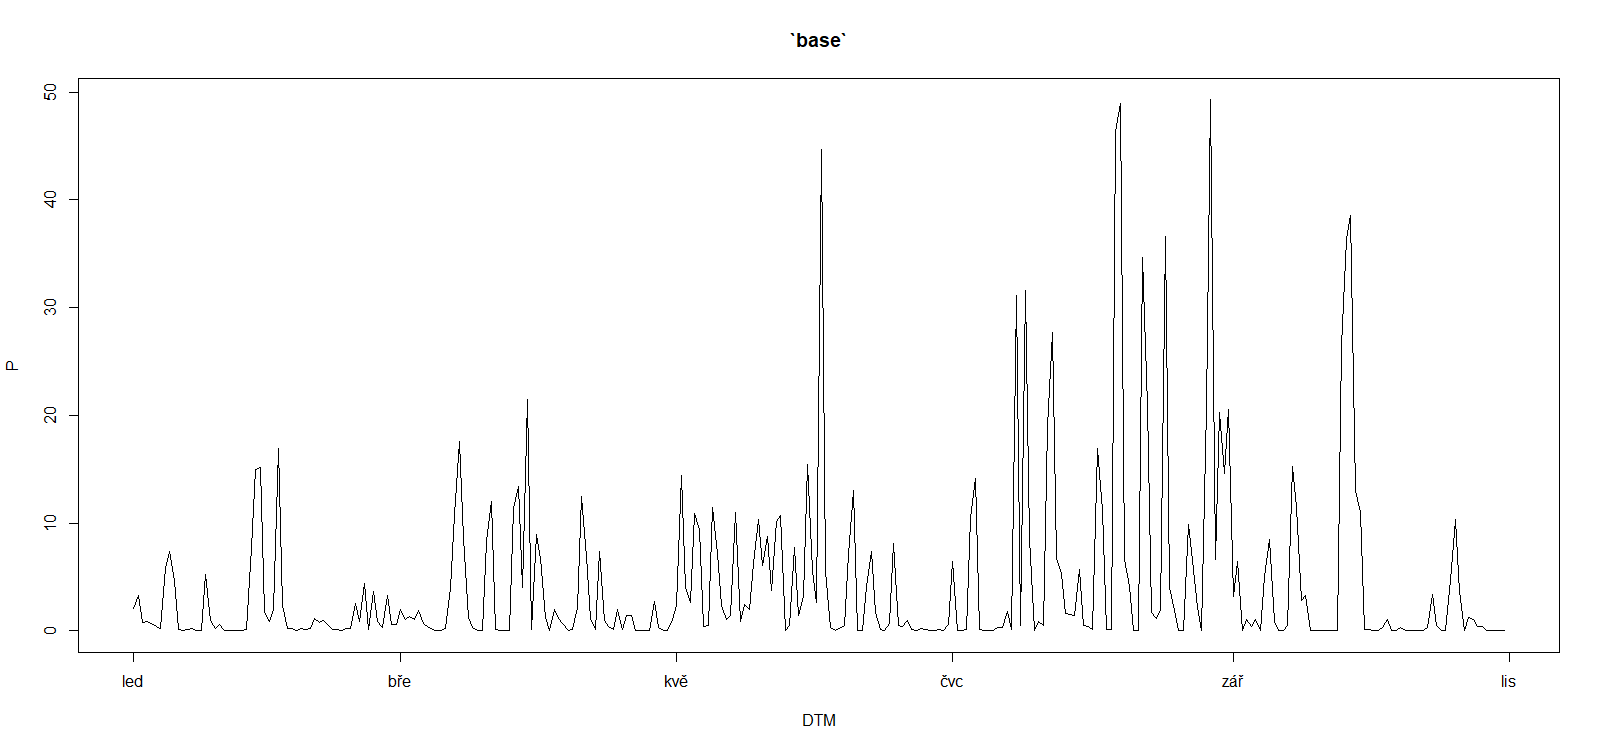
\includegraphics[width=\textwidth]{fig/1base}
      \caption{Časová řada srážek na zvoleným povodí v roce 2010, \texttt{base}}
      \label{fig1a}
\end{figure}

\newpage

\begin{Shaded}
\begin{Highlighting}[]
\KeywordTok{xyplot}\NormalTok{(P}\OperatorTok{~}\NormalTok{DTM, }\DataTypeTok{data =}\NormalTok{ HSL_}\DecValTok{0010}\NormalTok{, }\DataTypeTok{type =} \StringTok{"l"}\NormalTok{, }
                               \DataTypeTok{xlab =} \StringTok{"DTM"}\NormalTok{, }\DataTypeTok{ylab =} \StringTok{"P"}\NormalTok{, }
                               \DataTypeTok{main =} \StringTok{"`lattice`"}\NormalTok{ ,)}
\end{Highlighting}
\end{Shaded}

\begin{figure}[H]
      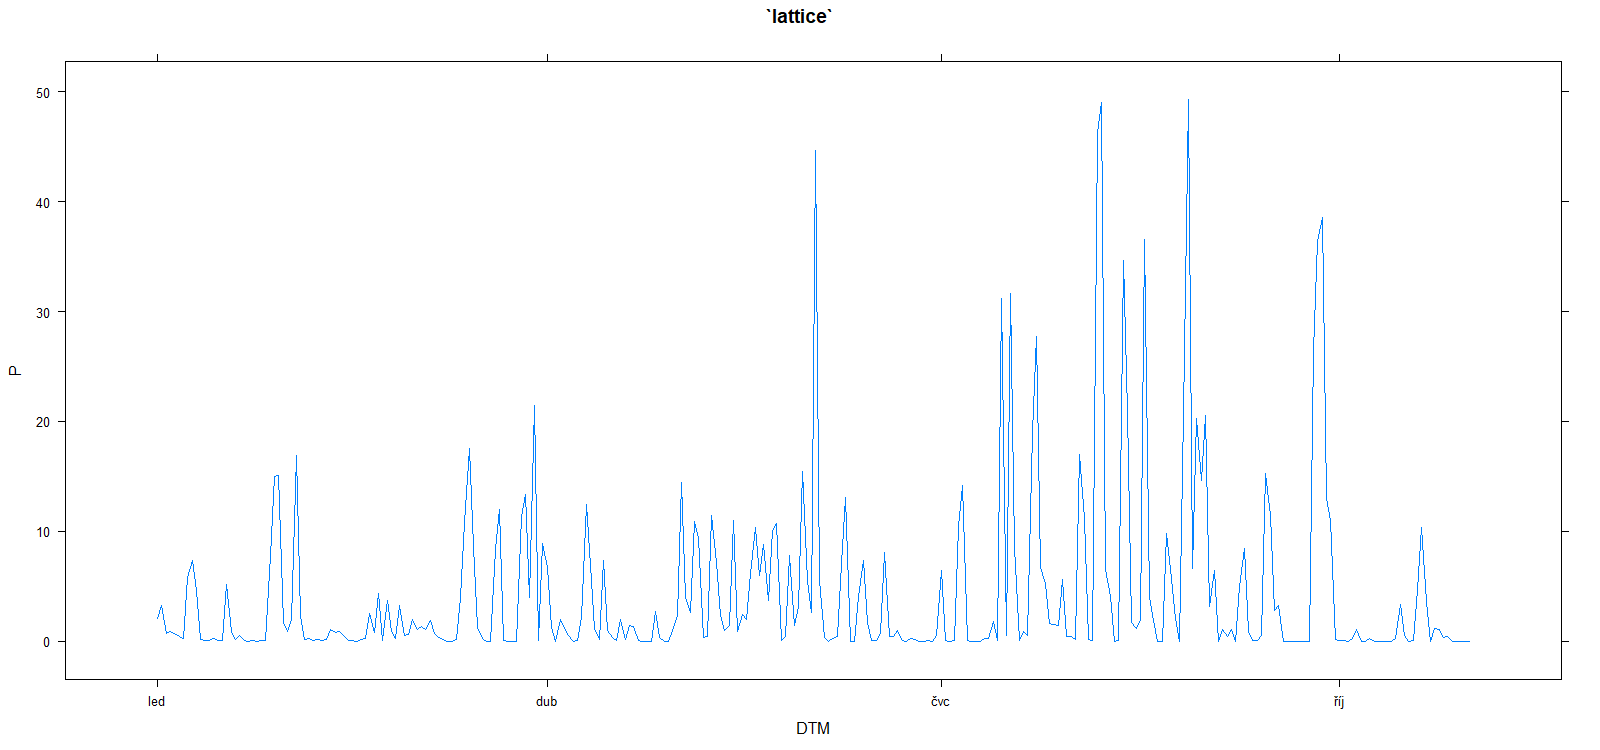
\includegraphics[width=\textwidth]{fig/2lattice}
      \caption{Časová řada srážek na zvoleným povodí v roce 2010, \texttt{lattice}}
      \label{fig1b}
\end{figure}

\begin{Shaded}
\begin{Highlighting}[]
\KeywordTok{ggplot}\NormalTok{(}\DataTypeTok{data=}\NormalTok{HSL_}\DecValTok{0010}\NormalTok{, }\KeywordTok{aes}\NormalTok{(DTM,P)) }\OperatorTok{+}\StringTok{ }
\StringTok{  }\KeywordTok{geom_line}\NormalTok{() }\OperatorTok{+}\StringTok{ }
\StringTok{  }\KeywordTok{labs}\NormalTok{(}\DataTypeTok{title =} \StringTok{"`ggplot2`"}\NormalTok{)}
\end{Highlighting}
\end{Shaded}

\begin{figure}[H]
      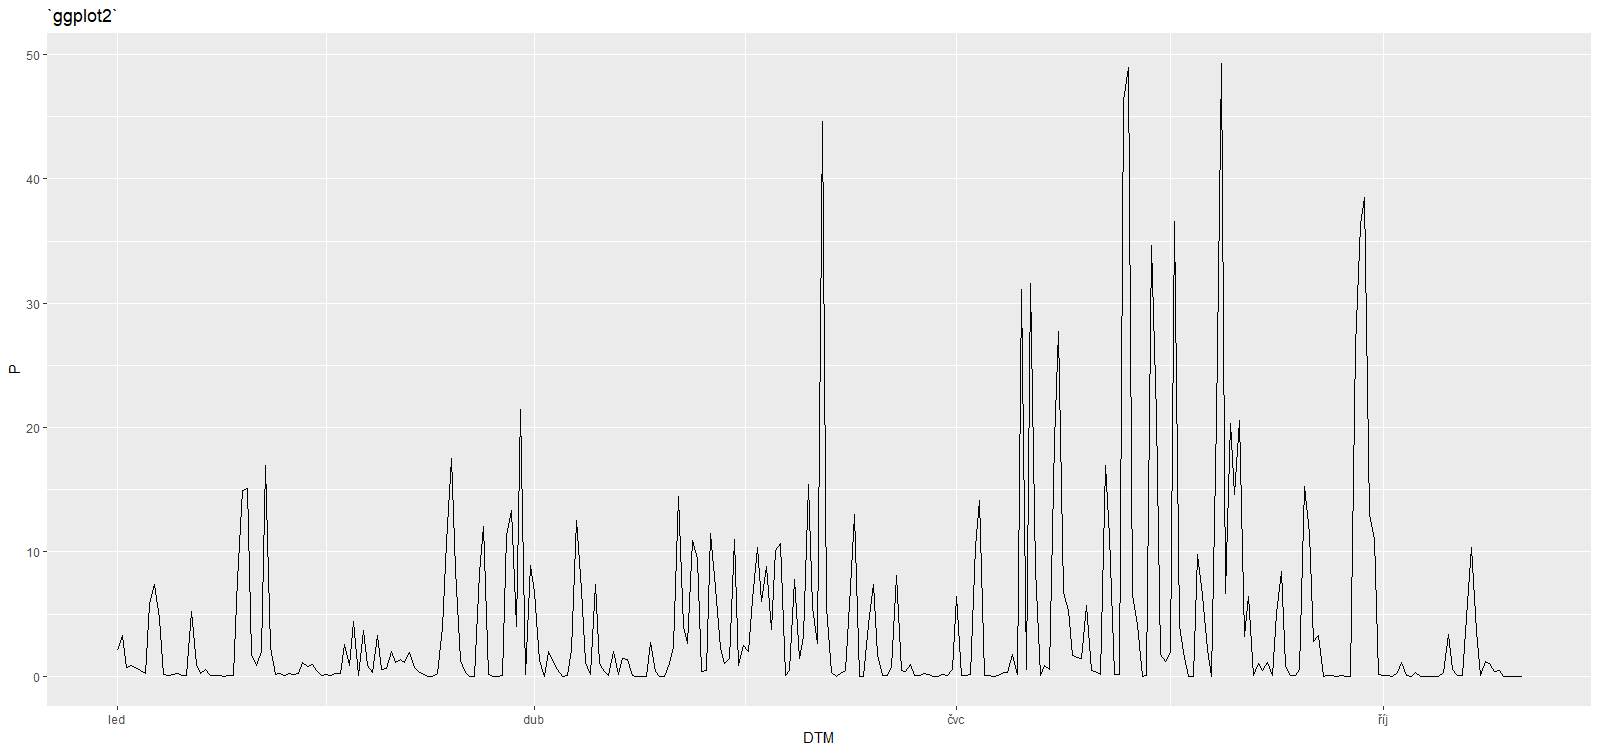
\includegraphics[width=\textwidth]{fig/3ggplot}
      \caption{Časová řada srážek na zvoleným povodí v roce 2010, \texttt{ggplot2}}
      \label{fig1c}
\end{figure}

\newpage

\subsubsection{4.2 Balíčky pro prostorovou
vizualizaci}\label{balicky-pro-prostorovou-vizualizaci}

\qquad V R existuje celá řada možností pro analýzu prostorových dat a
nástrojů k jejich vykreslení. Důležitý rozdíl mezi R a tradičními
desktopovými GIS (\emph{geographical information system}) softwary je
ten, že GIS je primárně vytvořen k prostorové vizualizaci a zpracovává
data jedním přednastaveným způsobem, zatímco v R uživatel si sám musí
zvolit vhodné nástroje a odpovídající nastavení. Dále R neobsahuje GUI,
které by usnadňoválo práci s prostorovými daty. Z tohoto důvodu může být
R pro nové uživatele naročné. Hlavní výhodou R je, že přínáší do tvorby
prostorové vizualizace silné výpočetní prostředky pro úpravu dat a
možnost uložení skriptů a jejich další modifikace. {[}43{]}

\begin{figure}[H]
  \centering
      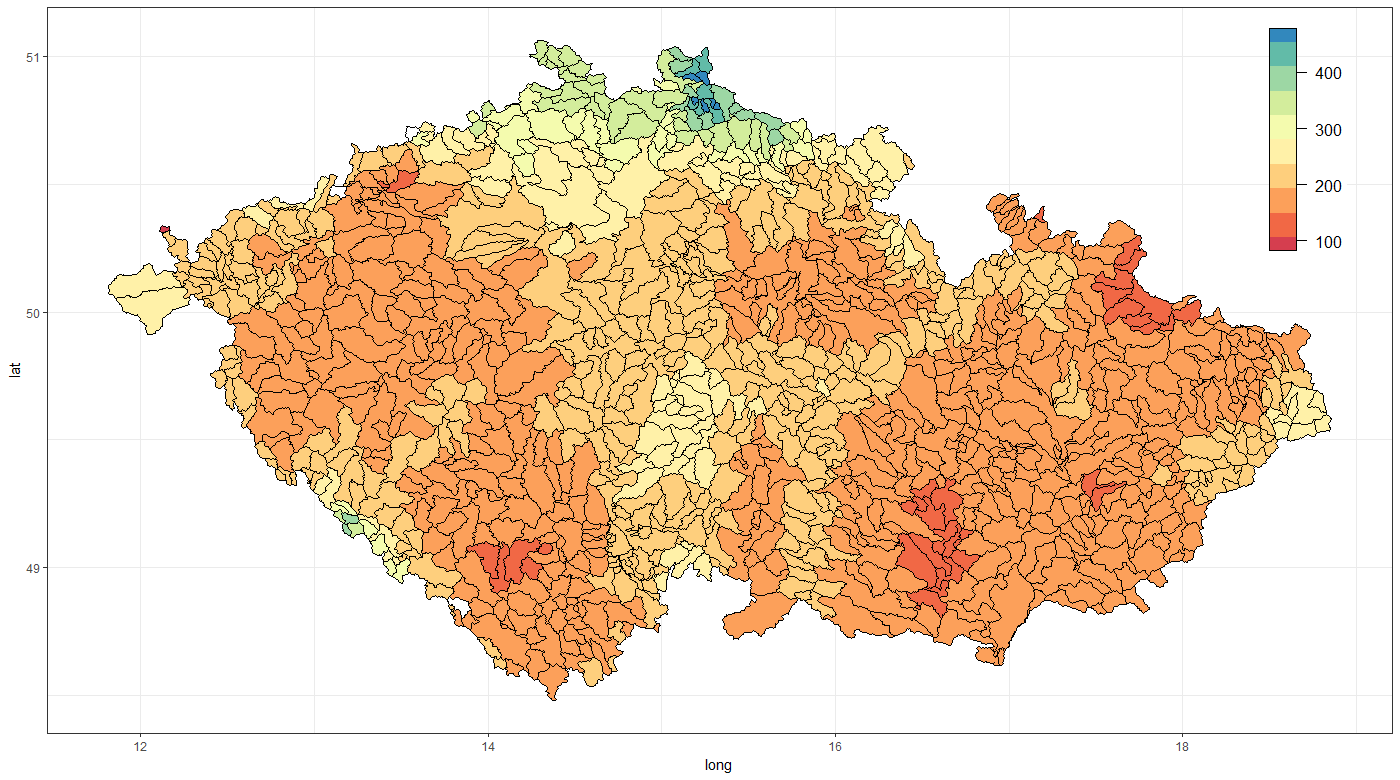
\includegraphics[width=\textwidth]{fig/ggplot_map2}
      \caption{Úhrn srážek (v mm) na povodích ČR za srpen 2010, vykresleno pomocí balíčků \texttt{ggplot2}}
      \label{fig02}
\end{figure}

\qquad Prostorové objekty jsou částo reprezentovány \emph{vektorovými}
daty. Takováto data obsahují popis \enquote{geometrie} nebo
\enquote{tvaru} území (body, linie a polygony) a většinou také obsahují
proměnné s dodatečnými informacemi o území. Dále se také používají
prostorová pole, která jsou obvýkle reprezentována pomocí \emph{rastrů}.
Rastrová data se obvykle použivají pro kontinuálná proměnné. Rastry dělí
území mřížkou na buňky o stejné velikosti neboli na \emph{pixely},
kterým je přiřazená hodnota dle zajmové proměnné. Většinou se jedná o
průměr či většinovou hodnotu pro oblast spadájící do konkretního pixelu.
Na rozdíl od vektorových dat, v rastrových datech není informace o
geometrii objektu uložená jako souřadnice, ale v rámci buňek. Velikost
rastrových buňěk neboli prostorové rozlišení je dáno počtem řadků a
sloupců, na které je území rozdělené. {[}44{]}

\qquad Vektorová data mohou být vykreslena v R pomocí celé řady balíčků
a to jak pomocí již zminěných \texttt{base} (kapitola
\protect\hyperlink{base}{4.1}) a \texttt{ggplot2} (kapitola
\protect\hyperlink{gg}{4.1.2}), tak i pomocí \texttt{Leaflet} (kapitola
\protect\hyperlink{leaflet}{4.3.3}). Příkladem vizualizace vektorových
dat pomocí balíčku \texttt{ggplot2} je zobrazeno na obrázku \ref{fig02}.

\begin{figure}[H]
  \centering
      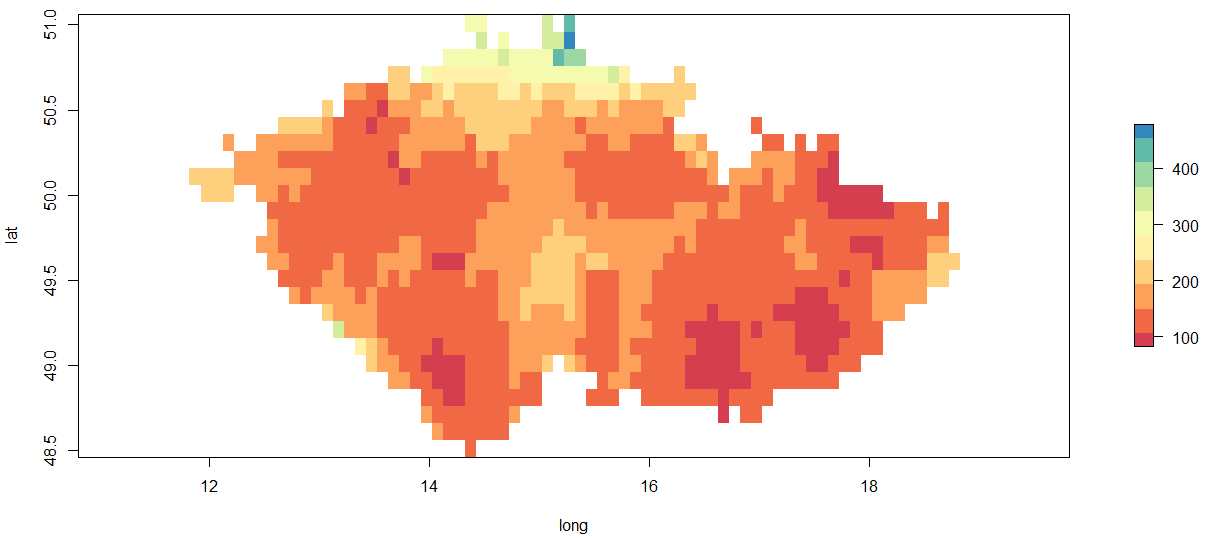
\includegraphics[width=\textwidth]{fig/raster_map2}
      \caption{Úhrn srážek (v mm) na povodích ČR za srpen 2010, vykresleno pomocí balíčků \texttt{raster}} 
      \label{fig03}
\end{figure}

\qquad Balíček \texttt{raster} obsahuje funkce pro vytvaření, čtení,
manipulaci, modelování, popis a analýzu rastrových dat. Podporuje prácí
s velkými soubory a vytvaření vlastních specifických funkcí. {[}45{]}
Balíček \texttt{rasterVis} představuje metody pro vylepšenou vizualizaci
a interakci s rastrovými daty. Implementuje vizualizační metody pro
kvantitativní a kvalitativní data a to jak pro jednorozměrné, tak i
vícerozměrné rastry. Dále poskytuje metody k zobrazení rastrů, měnících
se v čase, a vektorových polí.~{[}46{]} Vykreslení dat pomocí balíčku
\texttt{raster} lze nalézt na obrázku \ref{fig03}.

\subsubsection{4.3 Balíčky pro interaktivní vizualizaci
dat}\label{balicky-pro-interaktivni-vizualizaci-dat}

\qquad Možnost příblížit, filtrovat či zobrazit podrobnosti grafu na
požádání je výhodou dynamických a interakticních grafů. Interakticní
grafy dokažou zobrazovat více informací a tím umožňují i hlubší
pochopení dat. Pro R existuje široká nabídka balíčků a nástrojů k
vytváření interaktivních grafů. Jednou z nejpopulárnějších\footnote{Dle
  žebříčku \href{https://www.rdocumentation.org/}{rdocumentation.org} je
  \texttt{htmlwidgets} 58. nejstahovanější balíček.} možností je balíček
\texttt{htmlwidgets}, jehož knihovna obsahuje užitečné nástroje pro
tvorbu téměř jakéhokoliv typu grafiky.

\qquad Balíček \texttt{htmlwidgets} poskýtuje rozhrání pro snadné
propojení jazyku R a knihoven programovácího jazyku JavaScript,
používáného zejména pro webové aplikace. Tímto je umožněna bezproblemová
a konzistentní práce interaktivních map, grafů a tabulek a to jak v
dokumentech \texttt{R\ Markdown} a v aplikacích \texttt{Shiny} (kapitola
\protect\hyperlink{shiny}{4.4.2}), tak i v rámci samotného R Studio.
\texttt{htmlwidgets} umožňuje vytváření vlastních \emph{widgets}, ale
především nabízí řadů již vytvořených, například \texttt{Plotly},
\texttt{Leaflet} a \texttt{dygraphs}. Tyto nástroje jsou dostupné
nejenom pro R, ale i pro další programovácí jazyky (například Python).
{[}47{]}

\paragraph{\texorpdfstring{4.3.1
\texttt{Plotly}}{4.3.1 Plotly}}\label{plotly}

\qquad Balíček \texttt{Plotly} je vysokoúrovňové rozhrání pro open
source JavaScript vizualizační knihovnu \texttt{plotly.js}. Pro tvorbu
interaktivních vizualizací využívá jako základ balíček
\texttt{htmlwidgets}. Dále umožňuje jednoduchý převod \texttt{ggplot2}
grafů na interaktivní verzi. \texttt{Plotly} objekt lze vytvořit dvěmi
způsoby, a to pomocí funkce \texttt{plot\_ly()}, která převádí data na
\texttt{Plotly} objekt, případně pomocí funkce \texttt{ggplotly()},
která převádí \texttt{ggplot2} objekt na \texttt{Plotly} objekt. Bez
ohledu na to, jak je \texttt{Plotly} objekt vytvořen, výsledkem je
interaktivní vizualizace, která ve své přednastavené verzi obsahuje
nástrojovou líštu a umožňuje přiblížení a pohyb po vizualizaci. {[}48{]}

\paragraph{\texorpdfstring{4.3.2
\texttt{dygraphs}}{4.3.2 dygraphs}}\label{dygraphs}

\qquad Balíček \texttt{dygraphs} je R rozhráním pro práci s
JavaScriptovou vizualizační knihovnou \texttt{dygraphs}. Poskytuje
bohaté možnosti k vykreslení časových řad v R, včetně podpory
interaktivních funkcí. Mezi tyto funkce patří například {[}49{]}:

\begin{itemize}
\tightlist
\item
  Automatické vykreslení časových řad typu \texttt{xts}\footnote{Objekt
    \texttt{xts} pochází z balíčku \texttt{xts}, který je rozšířením
    populárního balíčku pro práci s časovými řadami \texttt{zoo}.}
\item
  Vysoce konfigurovatelná nastavení os a vykreslení řad (včetně
  volitelné další osy~\(y\))
\item
  Zvyraznění, přiblížení řad či bodů
\item
  Zobrázení predikčních interválů kolem řad
\item
  Umožnuje vykreslování překrývájících se grafů, vyznačení oblastí
  zastíněním a označení určitých událostí svislými liniemi a popisky.
\end{itemize}

\hypertarget{leaflet}{\paragraph{\texorpdfstring{4.3.3
\texttt{Leaflet}}{4.3.3 Leaflet}}\label{leaflet}}

\qquad \texttt{Leaflet} je další z populárních open source JavaScript
vizualizačních knihoven pro interaktivní mapy. Využívají ji takové
webové stránky jako jsou
\href{http://www.nytimes.com/projects/elections/2013/nyc-primary/mayor/map.html}{\emph{The
New York Times}} a
\href{http://www.washingtonpost.com/sf/local/2013/11/09/washington-a-world-apart/?utm_term=.906188040dc1}{\emph{The
Washington Post}}, ale i
\href{https://blog.github.com/2013-06-13-there-s-a-map-for-that/}{\emph{GitHub}}
a \href{https://www.flickr.com/map}{\emph{Flickr}}. \texttt{Leaflet} je
také využíván GIS platformami jako jsou
\href{http://www.openstreetmap.org/\#map=7/49.714/15.060}{\emph{OpenStreetMap}},
\href{https://www.mapbox.com/}{\emph{Mapbox}} a
\href{https://carto.com/}{\emph{CartoDB}}.

\qquad Tento R balíček umožňuje integrování a ovladání \texttt{Leaflet}
map. Mezi jeho funkce patří pohyb/přiblížení v rámci mapy, možnost
vytvářet mapy z libovolných kombinací (polygony, linie, markery, atd.).
Dále snadno vykresluje prostorové objekty z balíčků \texttt{sp} nebo
\texttt{sf} a datové soubory se sloupci zeměpisné šířky a délky.
\texttt{Leaflet} také poskytuje možnost ovládání interakcí v
\texttt{Shiny} aplikacích přes stavající hranice mapového výřezu či
reakce na kliknutí myši uživatelem. Umožňuje zobrazení map v nesférickým
Mercatorově zobrazení a má mnoho dalších funkcí a doplňků. {[}50{]}

\newpage

\subsubsection{4.4 Balíčky pro webové
aplikace}\label{balicky-pro-webove-aplikace}

\paragraph{\texorpdfstring{4.4.1
\texttt{flexdashboard}}{4.4.1 flexdashboard}}\label{flexdashboard}

\qquad \texttt{flexdashboard} slouží k publikaci dat a jejích přehledné
vizualizaci v rámci webového prohlížeče. Využívá \texttt{R\ Markdown} k
publikaci souvisejících vizualizací do jednotného zobrázení neboli
\emph{dashboard}u. Balíček podporuje široký výběr komponentů, včetně
\texttt{htmlwidgets}, \texttt{base}, \texttt{lattice} a \texttt{grid}
grafiky, tabulek, textových poznámek a dalších. Vyznačuje se mimo jiné i
jednoduchým a flexibilním nastavením samotného rozvržení dashboardu a to
definováním řadků a sloupců. Komponenty takového dashboardu se pak
inteligentně přizpůsobí oknu prohlížeče, případně obrazovce mobilního
zařízení. Dále balíček umožňuje nastavení a přepínání mezi jednotlivými
záložkami dashboardu. Pro dynamické vizualizace lze kombinovat
\texttt{flexdashboard} a \texttt{Shiny} aplikace.

\hypertarget{shiny}{\paragraph{\texorpdfstring{4.4.2
\texttt{Shiny}}{4.4.2 Shiny}}\label{shiny}}

\qquad \texttt{Shiny} je balíček, umožňující jednoduché vytváření
interaktivních webových aplikací kombinací výpočetních možností R s
interaktivitou moderních webových stránek. Pomocí \texttt{Shiny} lze
vytvořit jak samostatnou aplikaci, běžící na webových strankách, tak i
lokální aplikaci bežící v prostředí R. Vzhled \texttt{Shiny} aplikace
lze modifikovat pomocí kaskádových stylů\footnote{Kaskádové styly (CSS)
  jazyk určený pro popis vzhledu elementů napsaných ve značkovácích
  jazycích (například HTML).}. {[}51{]}

\qquad Strukturou se \texttt{Shiny} aplikace líší od běžných skriptů.
Celá aplikace by měla být umístěna v jednom adresáři a celý skript by
měl být obsažen v souboru nazvaném \texttt{app.R}.\footnote{V dřívějších
  verzích \texttt{Shiny} bylo nutné skript rozdělit do dvou částí
  \texttt{ui} a \texttt{server}.} Aplikaci pak lze spustit pomocí
příkazu \texttt{runApp("cesta")}, kde \texttt{cesta} je cesta k adresáři
s aplikací. Skript \texttt{app.R} se skládá ze tří komponentů:

\begin{itemize}
\tightlist
\item
  Uživatelské rozhraní \texttt{ui}, které obsahuje rozložení ovládacích
  prvků a nastavení vzhledu.
\item
  \texttt{server} funkce, který obsahuje funkce generující samotné
  interaktivní výstupy.
\item
  \texttt{ShinyApp} funkce, která spojuje \texttt{ui} a server. \newline
\end{itemize}

\begin{Shaded}
\begin{Highlighting}[]
\KeywordTok{library}\NormalTok{(shiny)}

\NormalTok{ui <-}\StringTok{ }\KeywordTok{fluidPage}\NormalTok{()}

\NormalTok{server <-}\StringTok{ }\ControlFlowTok{function}\NormalTok{(input, output)\{\}}

\KeywordTok{shinyApp}\NormalTok{(}\DataTypeTok{ui =}\NormalTok{ ui, }\DataTypeTok{server =}\NormalTok{ server)}
\end{Highlighting}
\end{Shaded}

\newpage

V rámci \texttt{ui} lze používat širokou řadu ovldácích prvků jako jsou
například tlačítka, zatrhávací políčka, přepínače, textové vstupy, atd.
Běžně se \texttt{ui} dělí do tří částí:

\begin{itemize}
\tightlist
\item
  Titulní panel, který obsahuje metadata, název aplikace a další
  relevantní informace.
\item
  Postraní panel, který nejčastěji obsahuje ovládací prvky.
\item
  Hlavní panel, který obsahuje výstupy generované funkcí
  \texttt{server}.
\end{itemize}

Příkladem ovladacího prvku vytvořeného v \texttt{ui} může být číselný
vstup, který umožňuje uživateli vložit libovolné číslo. Tento vstup je
označen pomocí \texttt{InputId} a v ramcí \texttt{server} funkcí lze na
něj dle toho id odkázat. Konkretně tento vstup lze získat z proměnné
\texttt{input\$num}. Obecně by to tedy mělo tvar
\texttt{input\$inputId}. Vstup z \texttt{ui} lze použit pouze v ramci
funkce \texttt{render*()}, případně v ramcí funkce \texttt{reactive()}
(viz dále).

\begin{Shaded}
\begin{Highlighting}[]
\NormalTok{ui <-}\StringTok{ }\KeywordTok{fluidPage}\NormalTok{(}\KeywordTok{numericInput}\NormalTok{(}\DataTypeTok{inputId =} \StringTok{"num"}\NormalTok{,}
                             \DataTypeTok{label =} \StringTok{"Číselný vstup"}\NormalTok{,}
                             \DataTypeTok{value =} \DecValTok{10}\NormalTok{))}
\end{Highlighting}
\end{Shaded}

Funkce \texttt{server} přebírá vstupy z ovládacích prvků \texttt{ui} a
mapuje jednotlivé funkce k výstupům. Příkladem takové funkce může být:

\begin{Shaded}
\begin{Highlighting}[]
\NormalTok{output}\OperatorTok{$}\NormalTok{histPlot <-}\StringTok{ }\KeywordTok{renderPlot}\NormalTok{(\{}
  \KeywordTok{hist}\NormalTok{(}\KeywordTok{rnorm}\NormalTok{(input}\OperatorTok{$}\NormalTok{num, }\DecValTok{1}\NormalTok{, }\DecValTok{0}\NormalTok{))}
\NormalTok{  \})}
\end{Highlighting}
\end{Shaded}

Tato funkce generuje grafický výstup v podobě histogramu normálního
rozdělení s interaktivním počtem pozorování. Obecně pro generování
výstupu se používá funkce \texttt{render*()}. Tyto funkce mohou
obsahovat libovolný kód (například příprava dat, doprovodné výpočty,
atd.), ale je nutné, aby vráceli požadovaný typ výstupu. Základní
\texttt{render*()} funkce jsou vypsáne v tabulce \ref{tab3}. Při změně
vstupu z \texttt{ui} v \texttt{render*()} dochází k přepočítání.

\begin{table}[H]
\centering
\begin{tabular}{@{}ll@{}}
\toprule
\multicolumn{1}{l}{Funkce}  & \multicolumn{1}{l}{Výstup}  \\ \midrule
\texttt{renderDataTable()}  & Interaktivní tabulka  \\
\texttt{renderImage()}  & Obrázek \\
\texttt{renderPlot()} & Graf  \\
\texttt{renderPrint()}  & Vytištěný blok kódu \\
\texttt{renderTable()}  & Tabulka  \\
\texttt{renderText()} & Text \\
\texttt{renderUI()} & \texttt{Shiny ui} element \\ \bottomrule
\end{tabular}
\caption{Základní \texttt{render*()} funkce}
\label{tab3}
\end{table}

\newpage

\qquad Pro komplexní \texttt{Shiny} aplikaci s větším počtem
interaktivních prvků je vhodné použit funkce \texttt{reactive()} (tzv
reaktivní výrazy). Tato funkce slouží zejména jako prostředník mezi
\texttt{ui} a \texttt{render*()}. Na obrázku \ref{fig04} je znazorněn
příklad struktury jednoduché \texttt{Shiny} aplikace s použítím
\texttt{reactive()} funkce. V tomto příkladu při změně numerického
vstupu (\texttt{input\$1}) se nejprvé přepočítá \texttt{reactive()} a
následně \texttt{render*()\ A} a \texttt{B}, zatímco při změně vstupu
\texttt{input\$2} či \texttt{input\$3} se přepočítají pouze přislušné
\texttt{render*()} výstupy \texttt{A} či \texttt{B} se zachováním
informací z \texttt{input\$1}.

\begin{figure}[H]
  \centering
      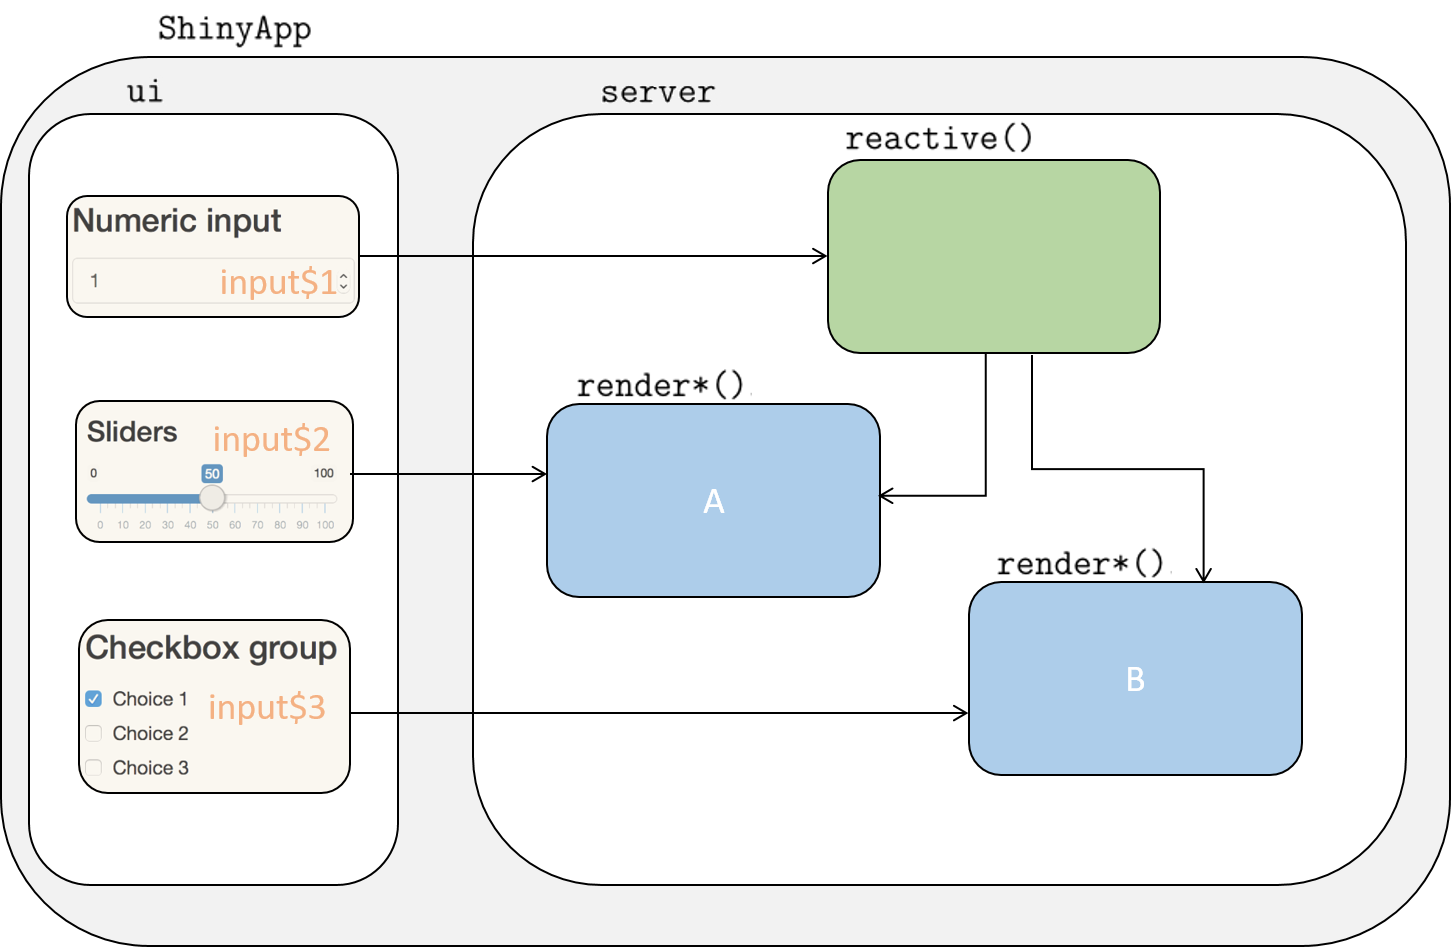
\includegraphics[width=\textwidth]{fig/shiny}
      \caption{Úkazka \texttt{Shiny} aplikace s použitím funkce \texttt{reactive()}.} 
      \label{fig04}
\end{figure}

\newpage

\section*{Praktická část}\label{prakticka-cast}
\addcontentsline{toc}{section}{Praktická část}

\subsection{5 Metodika}\label{metodika}

Aplikace je vytvořena prostřednictvím programovacího jazyka R. Jedná se
o vizualizaci výsledků modelování projektu \textbf{\emph{HAMR}} (viz
záložka \enquote{O projektu}). Jádro aplikace je postaveno na balíčcích
\texttt{Shiny} a \texttt{flexdashboard}.

\texttt{Shiny} umožňuje jednoduché vytváření webových aplikací,
interaktivních vizualizací v prostředí R. Balíček \texttt{flexdashboard}
je rozšířením \texttt{Shiny} a umožňuje pokročilé formátovaní vzhledu.
Společně slouží k publikaci dat a jejích přehledné vizualizaci v rámci
webového prohlížeče.

\subsubsection{5.1 Technické řešení}\label{technicke-reseni}

Aplikace je přístupná na
\href{https://shiny.fzp.czu.cz/KVHEM/HAMR/}{serveru}\footnote{\url{https://shiny.fzp.czu.cz/KVHEM/HAMR/}}
nebo ji lze také
\href{https://github.com/KVHEM/Sucho}{stáhnout}\footnote{\url{https://github.com/KVHEM/Sucho}}.
Repositář na \href{https://github.com/}{github}\footnote{\url{https://github.com/}}
obsahuje následující soubory:

\begin{itemize}
\tightlist
\item
  soubor s aplikací \enquote{flex\_app.Rmd}
\item
  skript připravující vstupní data pro aplikací \enquote{prep.R}
\item
  skript pro automatickou instalaci potřebných balíčku
  \enquote{install.packages.R}
\item
  soubor s kaskádovými styly pro nastavení vzhledu aplikace
  \enquote{styles.css}
\end{itemize}

Mimo již zmíněné balíčky \texttt{Shiny} a \texttt{flexdashboard} byly
použité následující balíčky:

\begin{itemize}
\tightlist
\item
  \texttt{leaflet}, umožňující vizualizaci prostorových dat v
  interaktivních mapách
\item
  \texttt{ggplot2}, \texttt{dygraphs} k vykreslení časových řad a čar
  překročení
\item
  \texttt{sp}, \texttt{rgeos} pro práci s prostorovými daty
\item
  \texttt{data.table}, \texttt{dplyr} sloužící k transformaci dat
\end{itemize}

\subsubsection{5.2 Postprocessing}\label{postprocessing}

Na základě kalibrovaných parametrů modelu Bilan jsou vygenerovány denní
časové řady odtoku a ostatních bilančních veličin pro období 1961-2015.
Pro aplikaci jsou dále vygenerovány další datové produkty:

\begin{itemize}
\tightlist
\item
  měsíční data - pro teplotu jsou průměry z denních hodnot, pro ostatní
  ukazatele jsou součty denních hodnot
\item
  data pro čáru překročení - pochází z měsíčních dat, které jsou řazeny
  dle celého období, měsíců a sezon
\end{itemize}

Na základě evidence užívání vod, kterou spravuje VÚV T. G. M., jsou
generovány měsíční časové řady pro období 2006-2016 a tabulky:

\begin{itemize}
\tightlist
\item
  data pro časovou řadu za vybrané povodí jsou sumami jednotlivých
  odběratelů seskupenými podle jevů
\item
  tabulka \enquote{Suma dle odběratele} obsahuje sumy za celé období za
  každého odběratele dle jevu
\end{itemize}

Aplikace pracuje s velkým množstvím dat, které se v rámci aplikace
filtrují, agregují a průměrují. Pro snížení výpočetního času a
náročnosti by bylo vhodné některé z těchto úkonů předpočítat a uložit
jako datový soubor Rds. Téměř všechny výpočty mohou být předpočítany,
ale implementace tohoto postupu proběhne v budoucnu. Je nutné nejdříve
změřit a kvantifikovat rozdíl ve výkonu před a po implementaci.

\subsection{6 Základní rozvržení}\label{zakladni-rozvrzeni}

\subsubsection{6.1 Základní mapa}\label{zakladni-mapa}

\begin{figure}[H]
      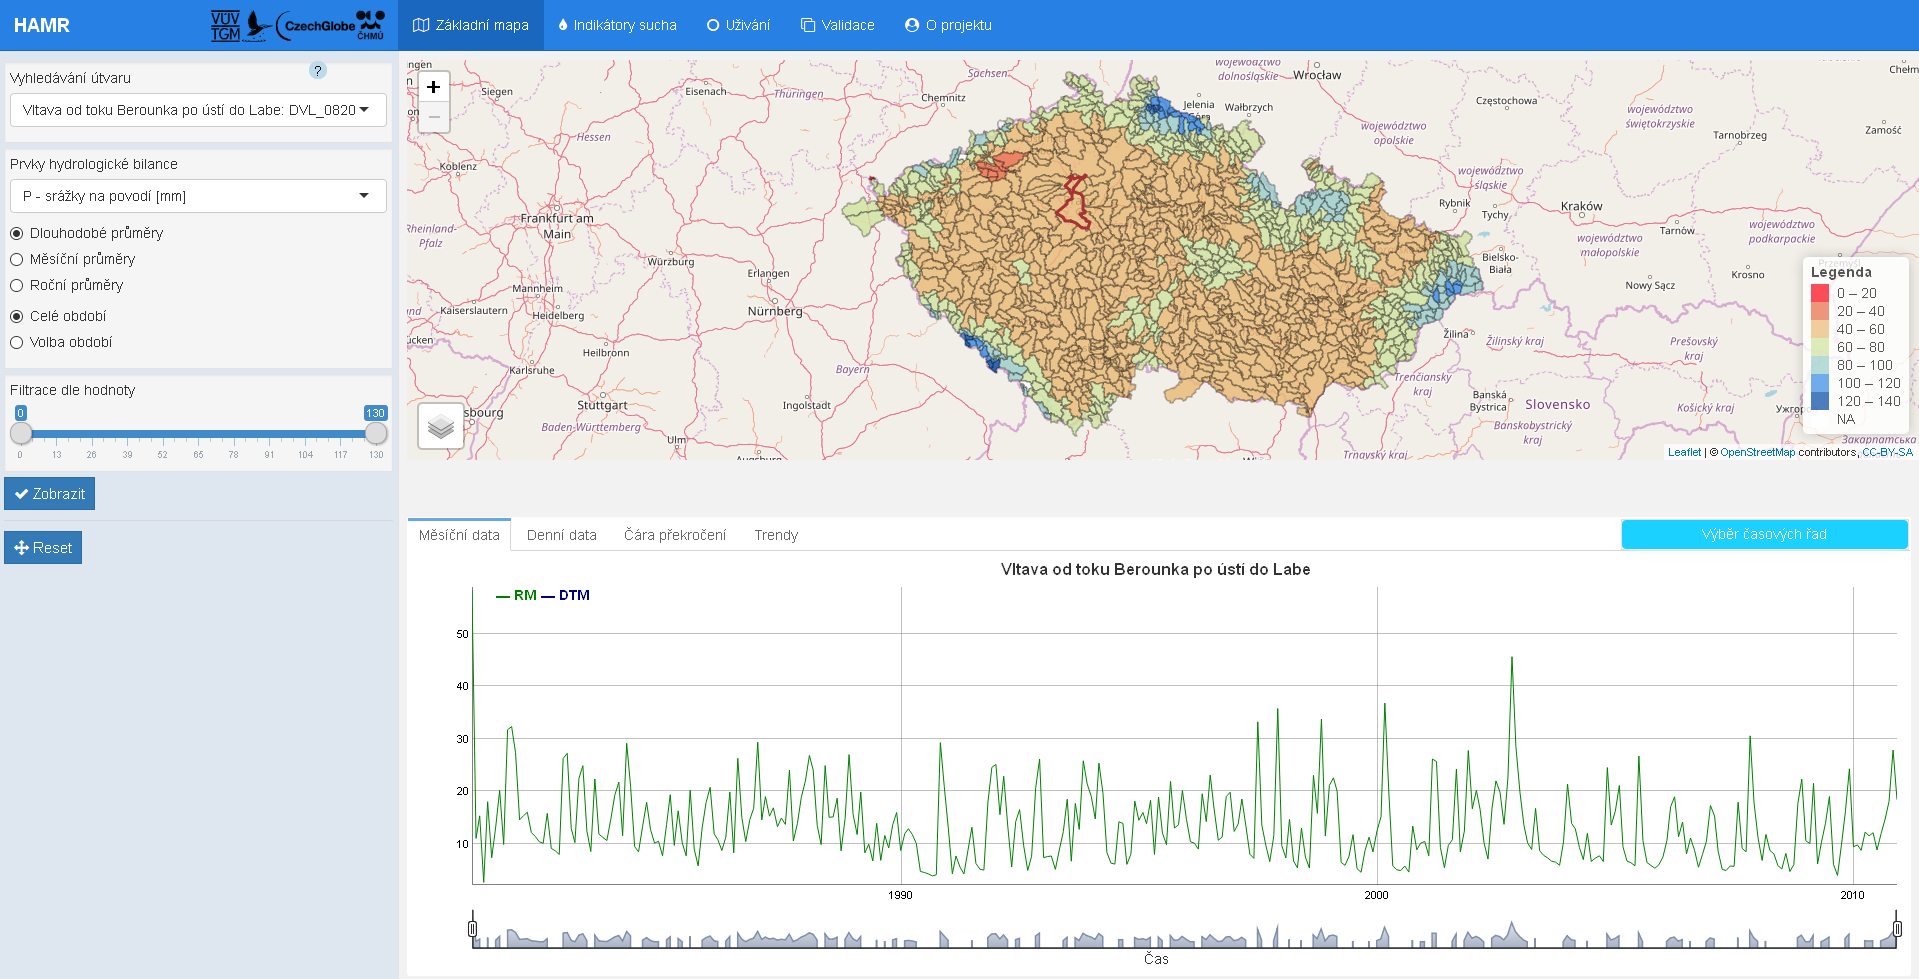
\includegraphics[width=\textwidth]{fig/P_ZM}
      \caption{Okno "základní mapa"}
      \label{fig1}
\end{figure}

Okno prohlížeče je rozděleno do tří části: boční panel, panel s mapovým
výstupem a panel s grafickými výstupy.

V bočním panelu se nastavují vstupy pro vykreslení mapy. Volí se zde
proměnná hydrologické bilance, podle níž budou zbarveny jednotlivá
povodí zobrazené na mapě. Hodnoty jsou agregovány do měsíčních a ročních
kroků, lze také vykreslit dlouhodobé průměry, tzn. průměry za celé
období a za periody 1961-1990, 1971-2000 a 1981-2010.

Filtrace dle hodnoty v počátečním stavu obsahuje všechny hodnoty zvolené
proměnné. Po nastavení rozsahu hodnot se vykreslí pouze povodí
odpovídající požadavku.

Vyhledávání útvaru je jedinou částí bočního panelu, která je propojená
nejenom s mapou, ale i s grafickými výstupy. Pro zvolené povodí se
vypočítají časové řady z měsíčních a denních dat a čára překročení pro
celé období, roční období a měsíce (dlouhodobé charakteristiky). Zvolené
povodí se zvýrazní v mapě červeným okrajem. Kliknutím na jiné povodí se
přepočítají grafické výstupy a název nově zvoleného povodí s jeho
UPOV\_ID se promítne do pole \enquote{Vyhledávání útvaru}. Toto pole lze
také použít k ručnímu vyhledávání; stačí vymazat momentálně zobrazený
název a začít psát název toku či jeho UPOV\_ID.

Grafy mají vlastní výběr proměnných z prvků hydrologické bilance, který
se nachází v pravém horním rohu grafického panelu.

Po nastavení údajů k vykreslení lze použít tlačítko \enquote{Zobrazit}.

Tlačítko \enquote{Reset} vrací mapový panel na počátečně nastavené
souřadnice

Mapový panel obsahuje základní vrstvy (jsou obsaženy v každém mapovém
výstupu aplikace), jsou to vrstvy řek, jezer a nádrží a vrstva mapového
podkladu. Vrstva povodí se zbarví dle nastavení v bočním panelu. Dále
jsou k dispozici vrstvy administrativního členění ČR, vrstva povodí 3.
řádu a vrstva horního povodí. Vrstva horního povodí zobrazuje pouze
povodí přitékající do vybraného povodí.

V budoucnu bude umožněno přiblížení zvoleného polygonu a jemu
odpovídacího okresu, kraje či oblasti povodí 3. řádu. Tento systém
přibližování by pak měl být použít i u ostatních mapových výstupů v
aplikaci.

Momentálně jsou v grafickém panelu u časových řad zobrazeny trendy pro
celé pozorované období. V budoucnu budou grafické výstupy rozšířeny o
záložku \enquote{Trendy}, kde bude umožněna vizualizace trendů a
vyhodnocení statistické významnosti pro vybrané období.

\subsubsection{6.2 Indikátory sucha}\label{indikatory-sucha}

\begin{figure}[H]
      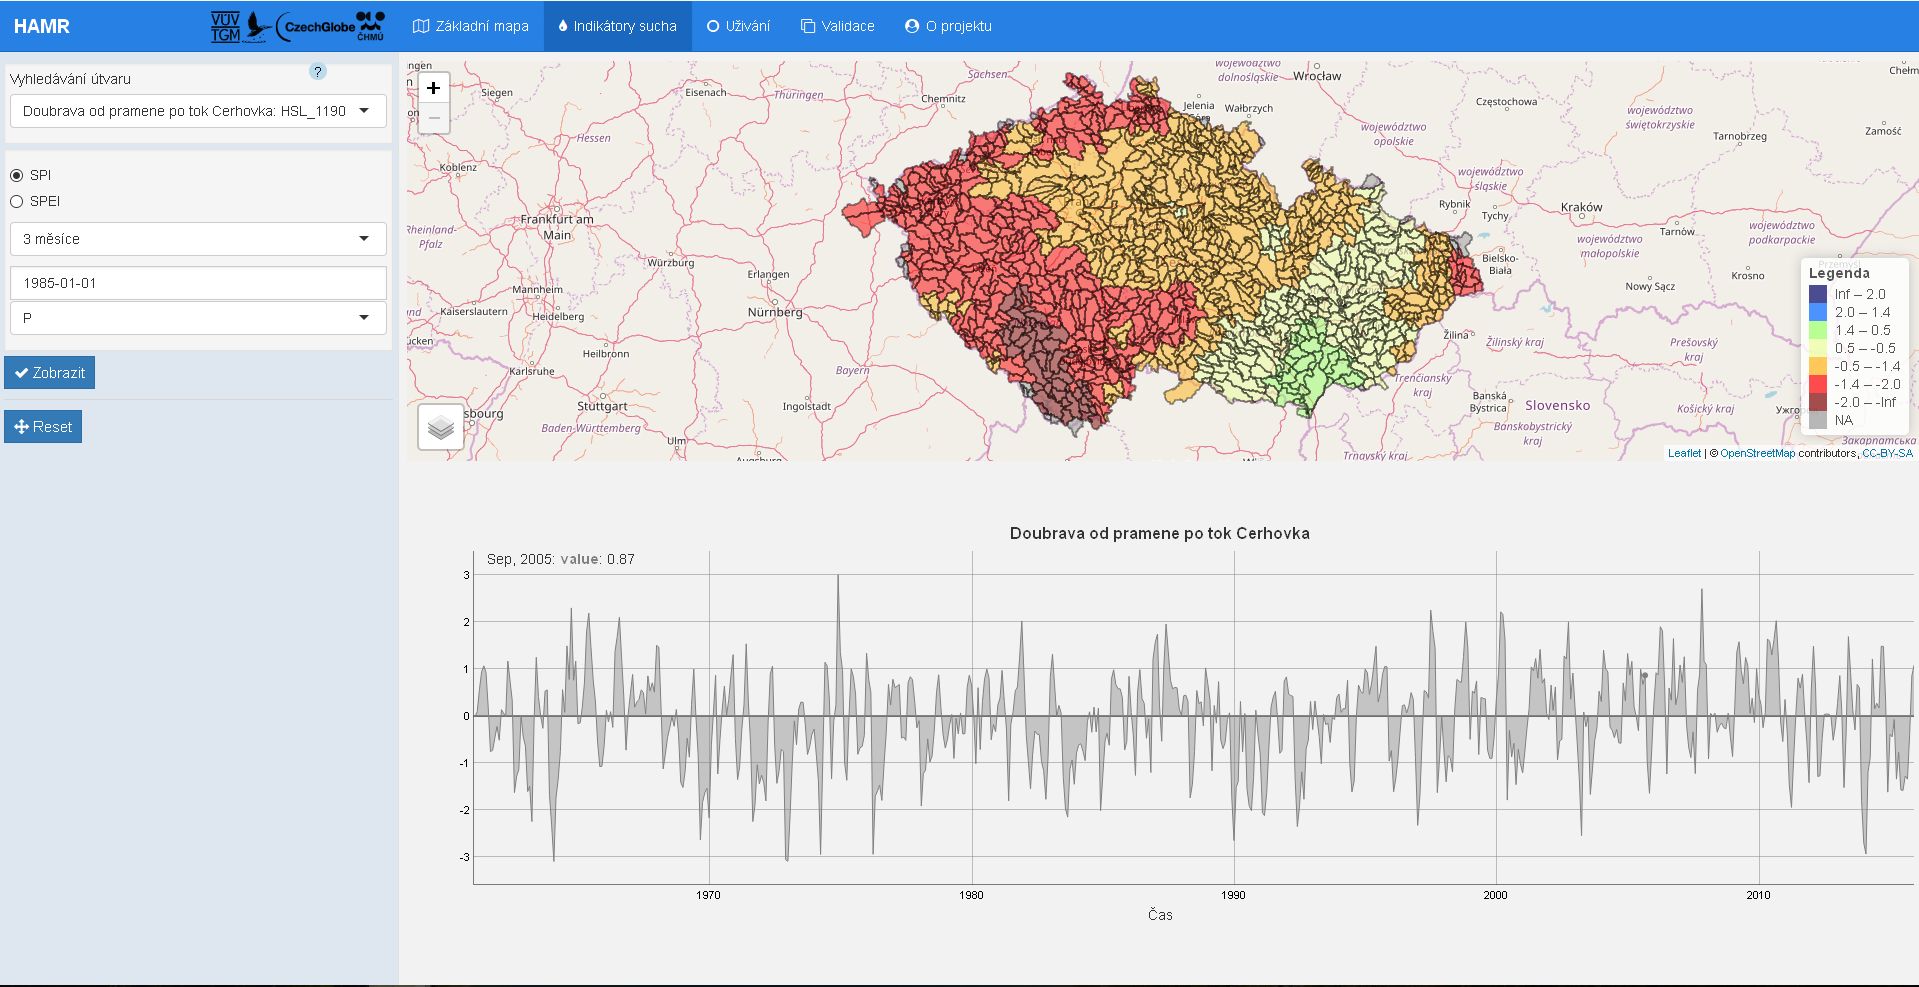
\includegraphics[width=\textwidth]{fig/P_indikatory}
      \caption{Okno "indikatory"}
      \label{fig2}
\end{figure}

Záložka indikátory sucha se skládá z bočního panelu, mapového panelu a
grafického panelu. V bočním panelu si lze zvolit indikátor, krok, do
kterého budou data agregována a datum. Momentálně v mapě je zobrazen
indikátor SPI počítány klouzavě s krokem 1, 3, 6 a 12 měsíců. Časem
budou přidány indikátory SPEI, PDSI, SGI, SRI a nedostatkové objemy ve
stejném kroku. Povodí se rozdělují do 4 kategorií dle hodnot indexu:

\begin{itemize}
\tightlist
\item
  0 - bez výskytu sucha (-0,7 a vyšší)
\item
  1 - slabé sucho (-0,8 až -1,3)
\item
  2 - silné sucho (-1,4 až -1,9)
\item
  3 - mimořádné sucho (- 2,0 a nižší)
\end{itemize}

V grafický panelu se vykresluje časová řada indikátoru v konkretním
povodí.

\subsubsection{6.3 Užívání}\label{uzivani}

\begin{figure}[H]
      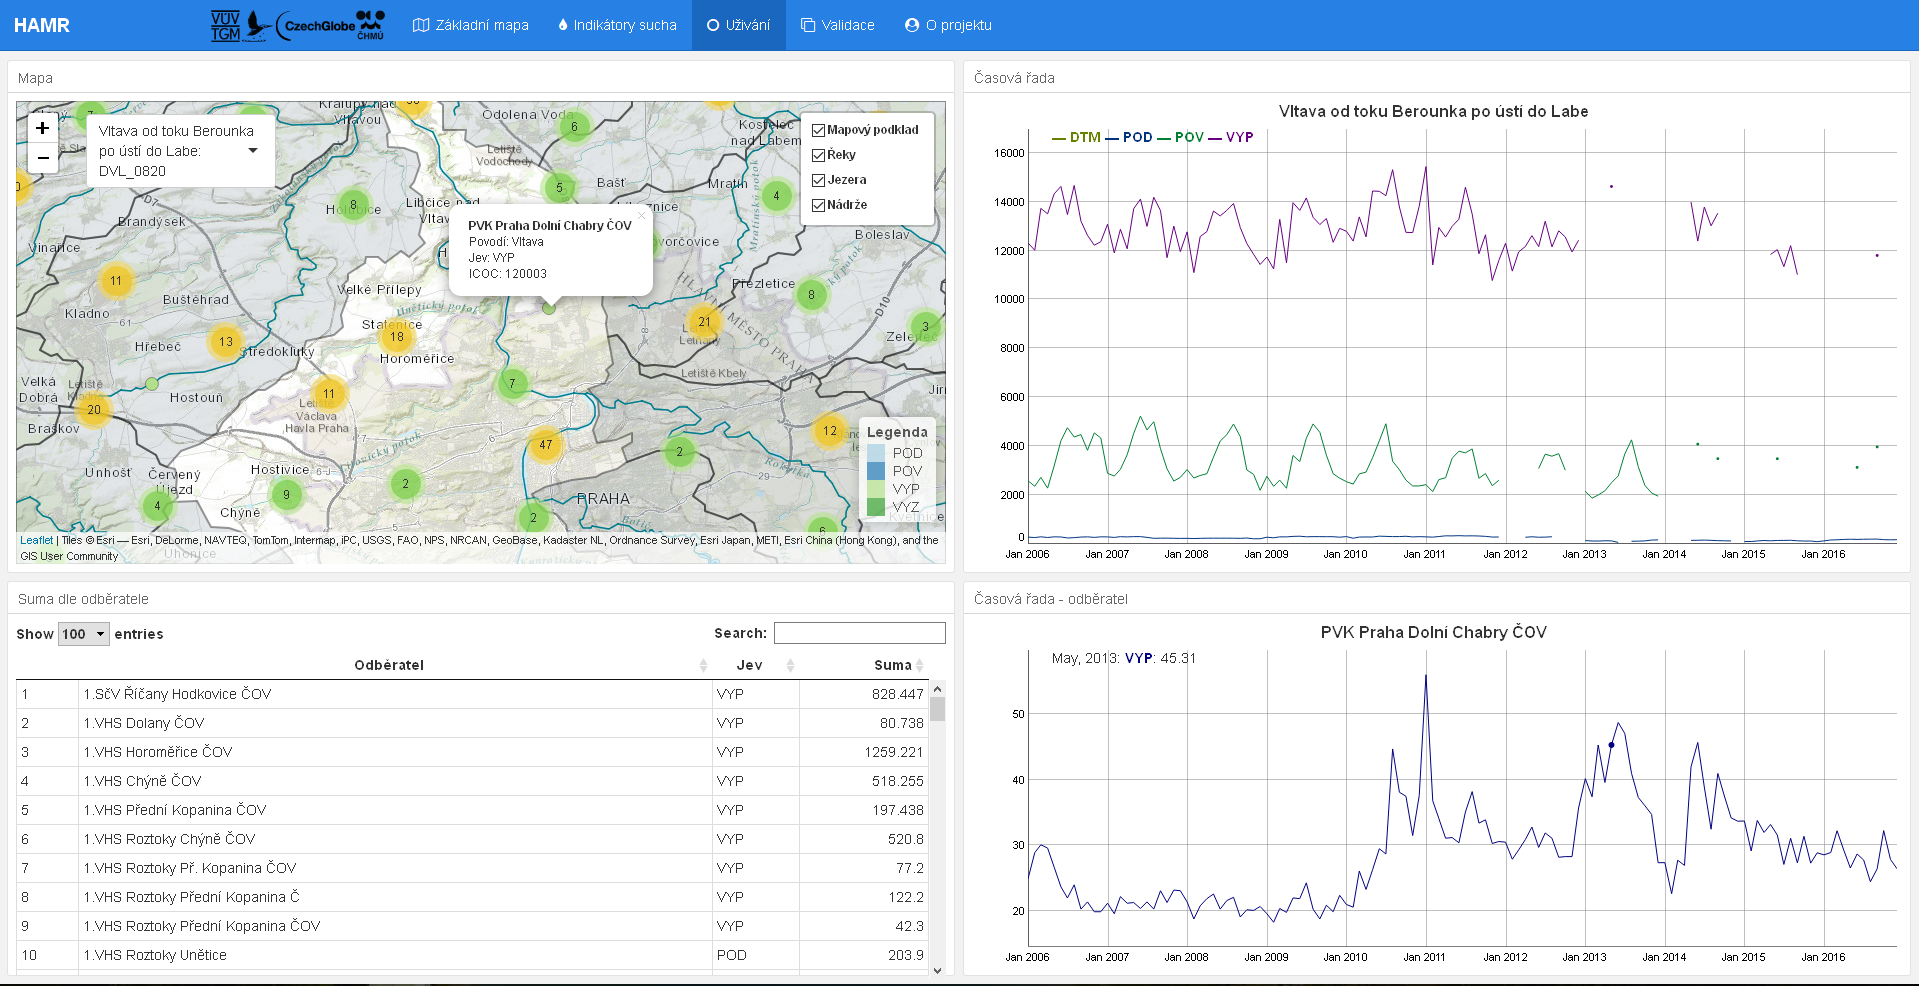
\includegraphics[width=\textwidth]{fig/P_uzivani}
      \caption{Okno "uzivani"}
      \label{fig3}
\end{figure}

Záložka užívání je rozdělena do čtyř části: panel s mapovým výstupem,
dva panely s grafickými výstupy a jeden panel s tabulkovým výstupem.

Mapový panel obsahuje informace o užívání vody v ČR. Místa užívání se
spojují do shluků. Po přiblížení lze na bod kliknout. Po kliknutí se
zobrazí informace o odběrateli a jeho časová řada. Kliknutím na povodí
je možno obdržet informace o všech odběratelích v tabulkovém panelu a
časovou řadu pro jednotlivé jevy v grafickém panelu.

Podobně jako v záložce \enquote{Základní mapa} zde existuje panel s
názvem povodí a jeho UPOV\_ID, ve kterém lze nalézt požadovaná povodí.
Tento panel lze přetáhnout na libovolné místo v rámci okna prohlížeče.

\subsubsection{6.4 Validace}\label{validace}

\begin{figure}[H]
      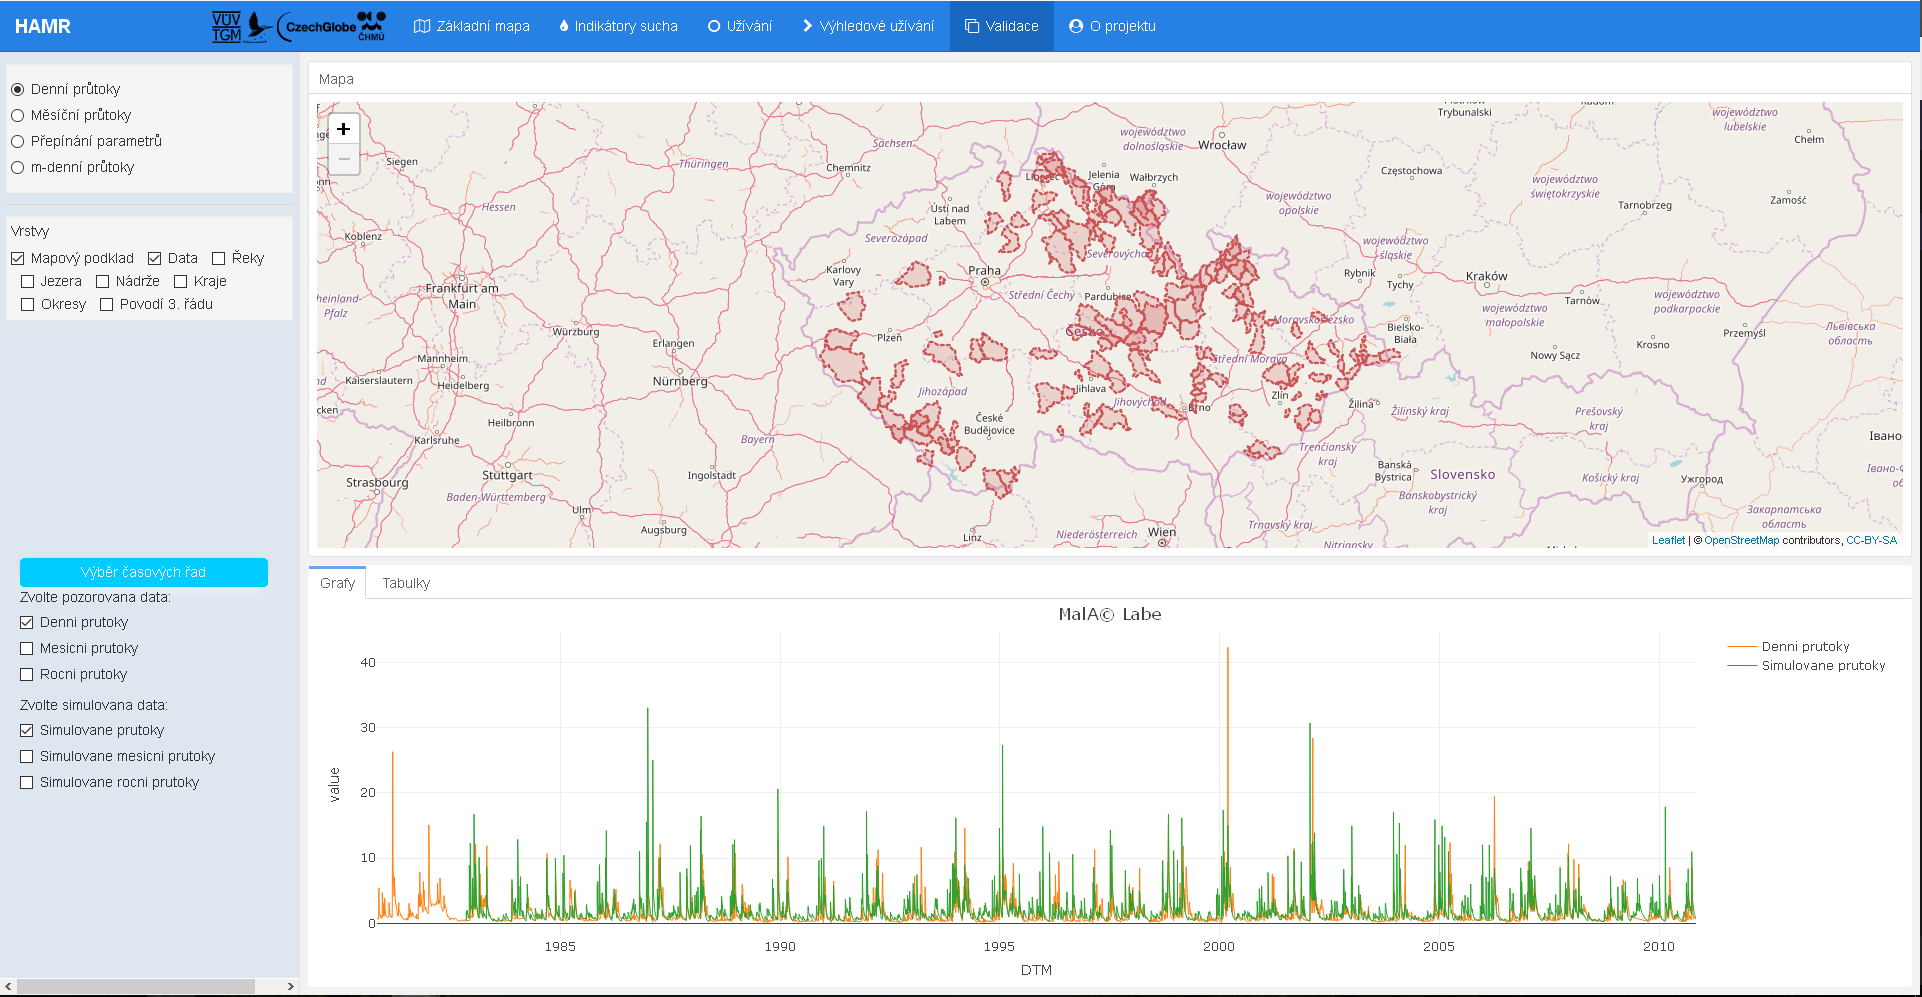
\includegraphics[width=\textwidth]{fig/P_validace}
      \caption{Okno "validace"}
      \label{fig4}
\end{figure}

V současné verzi záložka \enquote{Validace} se dělí na dvě částí: mapový
výstup denních průtoků/parametrů (lze přepnout v příslušném panelu) a
grafický panel s časovou řadou zvoleného povodí (lze vykreslit v denním,
měsíčním a ročním kroku pomocí panelu \enquote{Výběr časových řad}).

V dalších verzích bude umožněno porovnání výstupu modelu s pozorováním:

\begin{itemize}
\tightlist
\item
  ve vodoměrných stanicích
\item
  v profilech nádrží
\item
  charakteristiky UPOVu (m-denni vody)
\item
  plošné rozložení parametrů
\end{itemize}

\subsubsection{6.5 O projektu}\label{o-projektu}

\begin{figure}[H]
      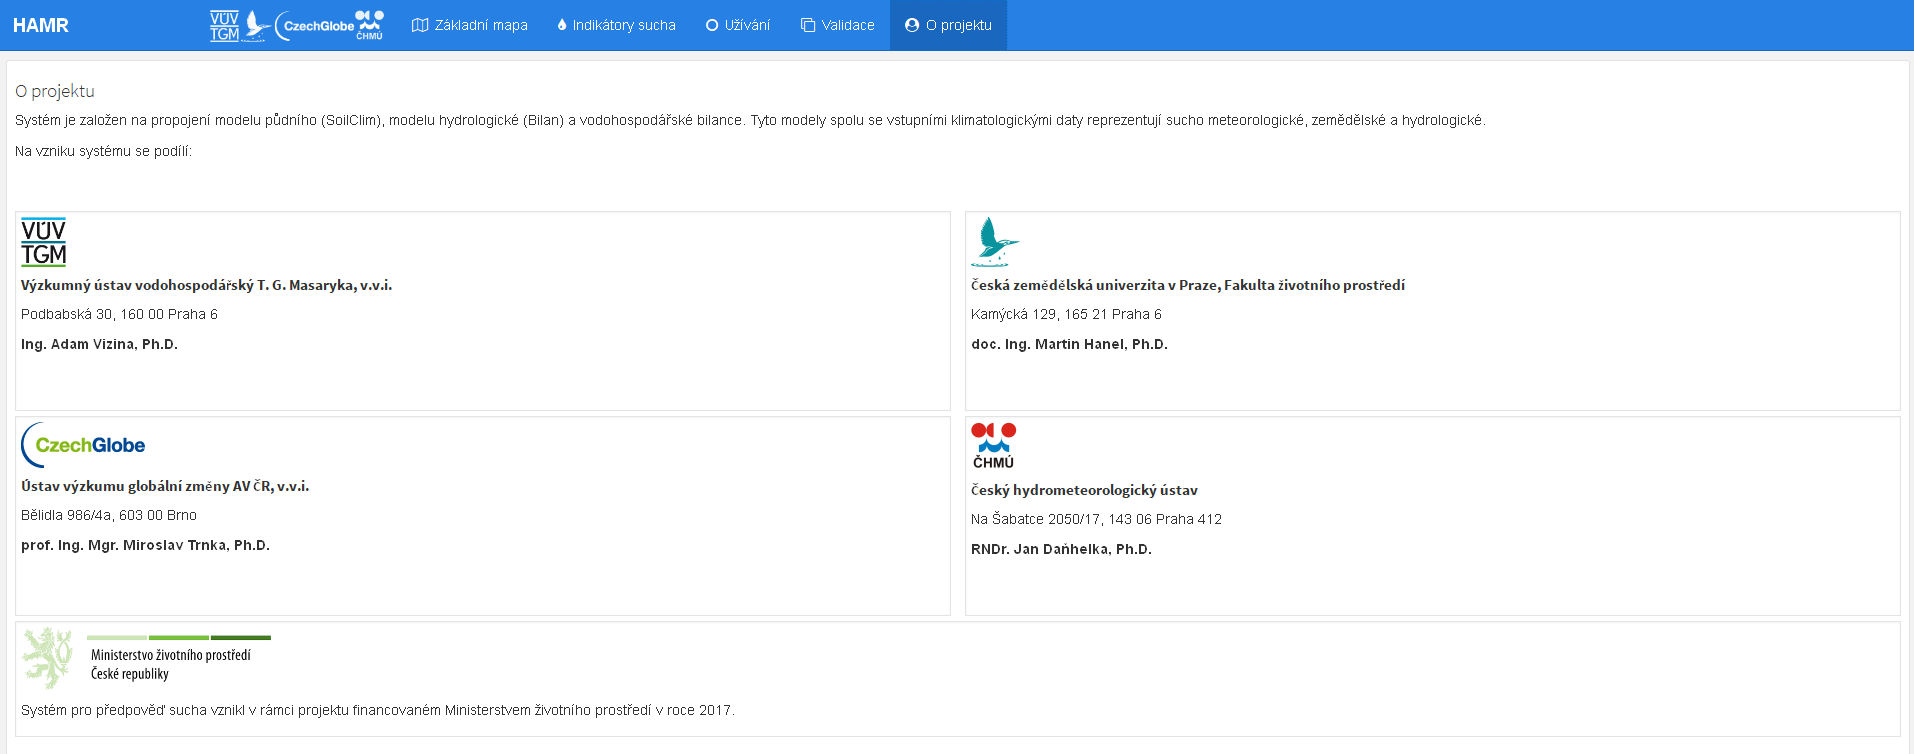
\includegraphics[width=\textwidth]{fig/P_o_projektu}
      \caption{Okno "o projektu"}
      \label{fig5}
\end{figure}

Krátký popis projektu a veškeré kontakty.V budoucnu bude rozšířeno o
metodiky k jednotlivým součástem systému.

\newpage

\section*{Výsledky}\label{vysledky}
\addcontentsline{toc}{section}{Výsledky}

\newpage

\section*{Diskuse}\label{diskuse}
\addcontentsline{toc}{section}{Diskuse}

\newpage

\section*{Závěr}\label{zaver}
\addcontentsline{toc}{section}{Závěr}

\newpage

\section*{Přílohy}\label{prilohy}
\addcontentsline{toc}{section}{Přílohy}

\addcontentsline{toc}{subsection}{\listfigurename}

\listoffigures

\newpage

\subsection{R kód}\label{r-kod}

\newpage

\subsection*{Literatura}\label{literatura}
\addcontentsline{toc}{subsection}{Literatura}

\hypertarget{refs}{}
\hypertarget{ref-dataviz_history}{}
{[}1{]} FRIENDLY, M. A Brief History of Data Visualization. In:
\emph{Handbook of Computational Statistics: Data Visualization}. B.m.:
Springer-Verlag, 2006. ISBN 978-3-540-32825-4.

\hypertarget{ref-brinton_1919}{}
{[}2{]} BRINTON, W.C. \emph{Graphic Methods for Presenting Facts}. B.m.:
The Engineering Magazine Company, New York, 1919. ISBN 978-1155058870.

\hypertarget{ref-tukey1962}{}
{[}3{]} TUKEY, J.W. The Future of Data Analysis. \emph{Annals of
Mathematical Statistics}. 1962.

\hypertarget{ref-tukey1977}{}
{[}4{]} TUKEY, J.W. \emph{Exploratory Data Analysis}. B.m.:
Addison-Wesley, 1977. ISBN 0201076160.

\hypertarget{ref-cleveland_priceonomics}{}
{[}5{]} \emph{How William Cleveland Turned Data Visualization Into a
Science {[}vid. 2.11.2017{]}} {[}online{]}. Dostupné z:
\url{https://priceonomics.com/}

\hypertarget{ref-datavis_rahlf}{}
{[}6{]} RAHLF, T. \emph{Data Visualisation with R: 100 Examples}. B.m.:
Springer, 2017. ISBN 978-3-319-49751-8.

\hypertarget{ref-tufte1990}{}
{[}7{]} TUFTE, E.R. \emph{Envisioning Information}. B.m.: Graphics Pr,
1990. ISBN 978-0961392116.

\hypertarget{ref-tufte1983}{}
{[}8{]} TUFTE, E.R. \emph{The Visual Display of Quantitative
Information}. B.m.: Graphics Press, 1983. ISBN 978-0961392109.

\hypertarget{ref-cleveland_mcgill}{}
{[}9{]} CLEVELAND, W.S. a R. MCGILL. Graphical Perception: Theory,
Experimentation, and Application to the Development of Graphical
Methods. \emph{Journal of the American Statistical Association}. 1984.

\hypertarget{ref-cleveland1994}{}
{[}10{]} CLEVELAND, W.S. \emph{The Elements of Graphing Data}. B.m.:
Hobart Press, 1994. ISBN 0963488414.

\hypertarget{ref-trellisplot}{}
{[}11{]} BECKER, R.A., W.S. CLEVELAND, M.-J. SHYU, aj. A tour of Trellis
graphics. \emph{Murray Hill, NJ: AT \& T Bell Laboratories}. 1996.

\hypertarget{ref-wilkinson2005}{}
{[}12{]} WILKINSON, L. \emph{The Grammar of Graphics}. B.m.: Springer,
2005. ISBN 9780387286952.

\hypertarget{ref-wickham_ggplot}{}
{[}13{]} WICKHAM, H. \emph{ggplot2: Elegant Graphics for Data Analysis
(Use R!)}. B.m.: Springer, 2010. ISBN 978-0387981406.

\hypertarget{ref-layered-grammar}{}
{[}14{]} WICKHAM, H. A layered grammar of graphics. \emph{Journal of
Computational and Graphical Statistics}. 2010.

\hypertarget{ref-cleveland1993}{}
{[}15{]} CLEVELAND, W.S. \emph{Visualizing Data}. B.m.: Hobart Press,
1993. ISBN 978-0963488404.

\hypertarget{ref-murray}{}
{[}16{]} MURRAY, S. \emph{Interactive Data Visualization for the Web}.
B.m.: O'Reilly Media, 2013. ISBN 978-1449339739.

\hypertarget{ref-ferster}{}
{[}17{]} FERSTER, B. \emph{Interactive Visualization: Insight through
Inquiry (MIT Press)}. B.m.: The MIT Press, 2012. ISBN 978-0262018159.

\hypertarget{ref-graphics}{}
{[}18{]} \emph{R: The R Graphics Package {[}vid. 22.4.2017{]}}
{[}online{]}. Dostupné z:
\url{https://stat.ethz.ch/R-manual/R-devel/library/graphics/html/graphics-package.html}

\hypertarget{ref-teetor2011}{}
{[}19{]} TEETOR, P. \emph{R Cookbook: Proven Recipes for Data Analysis,
Statistics, and Graphics}. B.m.: O'Reilly Media, 2011. ISBN
9781449307264.

\hypertarget{ref-plot}{}
{[}20{]} \emph{R: Generic X-Y Plotting {[}vid. 11.5.2017{]}}
{[}online{]}. Dostupné z:
\url{https://stat.ethz.ch/R-manual/R-devel/library/graphics/html/plot.html}

\hypertarget{ref-pp_wiki}{}
{[}21{]} \emph{P--P plot - Wikipedia {[}vid. 11.8.2017{]}} {[}online{]}.
Dostupné z: \url{https://en.wikipedia.org/wiki/P\%E2\%80\%93P_plot}

\hypertarget{ref-chang2012}{}
{[}22{]} CHANG, W. \emph{R Graphics Cookbook: Practical Recipes for
Visualizing Data}. B.m.: O'Reilly Media, 2012. ISBN 9781449363116.

\hypertarget{ref-novovic2006}{}
{[}23{]} NOVOVIČOVÁ, J. \emph{Pravděpodobnost a matematická statistika}.
B.m.: Praha: Vydavatelství ČVUT, 2006. ISBN 80-01-01980-2.

\hypertarget{ref-datarep2011}{}
{[}24{]} MACIEJEWSKI, R. \emph{Data Representations, Transformations,
and Statistics for Visual Reasoning}. B.m.: Morgan \& Claypool
Publishers, 2011. ISBN 978-1-608-45625-3.

\hypertarget{ref-hist_wiki}{}
{[}25{]} \emph{Histogram - Wikipedia {[}vid. 6.8.2017{]}} {[}online{]}.
Dostupné z: \url{https://en.wikipedia.org/wiki/Histogram}

\hypertarget{ref-grolemund_wickham2017}{}
{[}26{]} WICKHAM, H. a G. GROLEMUND. \emph{R for Data Science}. B.m.:
O'Reilly Media, 2017. ISBN 1491910399.

\hypertarget{ref-jackknife_tukey}{}
{[}27{]} TUKEY, J.W. Bias and Confidence in Not Quite Large Samples.
\emph{Annals of Mathematical Statistics}. 1958, roč. 29.

\hypertarget{ref-bootstrap}{}
{[}28{]} EFRON, B. a R. TIBSHIRANI. \emph{An Introduction to the
Bootstrap}. B.m.: Taylor \& Francis Ltd, 1994. ISBN 0-412-04231-2.

\hypertarget{ref-mcintosh2016}{}
{[}29{]} MCINTOSH, A. The Jackknife Estimation Method. \emph{arXiv}.
2016.

\hypertarget{ref-mbdist2}{}
{[}30{]} DE MAESSCHALCK, R., D. JOUAN-RIMBAUD a D.L. MASSART. The
mahalanobis distance. \emph{Chemometrics and intelligent laboratory
systems}. 2000, roč. 50, č. 1.

\hypertarget{ref-mbdist}{}
{[}31{]} MAHALANOBIS, P.C. On the generalised distance in statistics.
\emph{Proceedings National Institute of Science}. 1936.

\hypertarget{ref-leverages_regression}{}
{[}32{]} CARDINALI, C. Observation influence diagnostic of a data
assimilation system. \emph{Advanced Data Assimilation for Geosciences:
Lecture Notes of the Les Houches School of Physics: Special Issue}.
2014.

\hypertarget{ref-pecakova}{}
{[}33{]} PECÁKOVÁ, I. Problém chybějících dat v dotazníkových šetřeních.
\emph{Politická ekonomie}. 2014. ISSN 2336-8225.

\hypertarget{ref-transformation}{}
{[}34{]} \emph{Transformation of Data {[}vid. 3.2.2018{]}} {[}online{]}.
Dostupné z:
\url{http://statisticalconcepts.blogspot.cz/2010/02/transformation-of-data-validity-of.html}

\hypertarget{ref-vicerozm_stat}{}
{[}35{]} HEBÁK, P., J. HUSTOPECKÝ, E. JAROŠOVÁ, aj. \emph{Vícerozměrné
statistické metody (1)}. B.m.: Informatorium, Praha, 2007. ISBN
80-7333-025-3.

\hypertarget{ref-normalizing}{}
{[}36{]} ABDI, H. a L. WILLIAMS. Normalizing data. Encyclopedia of
research design. \emph{Thousand Oaks, CA: Sage}. 2010.

\hypertarget{ref-zumel_2014}{}
{[}37{]} ZUMEL, N. a J. MOUNT. \emph{Practical Data Science with R}.
B.m.: Manning, 2014. ISBN 9781617291562.

\hypertarget{ref-kutner_transform}{}
{[}38{]} KUTNER, M.H., C.J. NACHTSHEIM, J. NETER, aj. \emph{Applied
Linear Statistical Models}. B.m.: McGraw-Hill/Irwin, 2004. ISBN
0-07-238688-6.

\hypertarget{ref-SW_test}{}
{[}39{]} SHAPIRO, S.S. a M.B. WILK. An analysis of variance test for
normality (complete samples)†. \emph{Biometrika}. 1965.

\hypertarget{ref-normality_tests}{}
{[}40{]} ÖZTUNA, D., A.H. ELHAN a E. TÜCCAR. Investigation of four
different normality tests in terms of type 1 error rate and power under
different distributions. \emph{Turkish Journal of Medical Sciences}.
2006.

\hypertarget{ref-murrell1998}{}
{[}41{]} MURRELL, P.R. \emph{Investigations in Graphical Statistics}.
B.m., 1998. PhD thesis. The University of Auckland.

\hypertarget{ref-murrell2003}{}
{[}42{]} MURRELL, P. \emph{grid: The grid graphics package}. červenec
2003

\hypertarget{ref-spatial}{}
{[}43{]} CHESHIRE, J. a R. LOVELACE. Spatial data visualisation with R.
\emph{Geocomputation: A Practical Primer}. 2015.

\hypertarget{ref-spatial2}{}
{[}44{]} HIJMANS, R. \emph{Spatial Data Analysis and Modeling with R
{[}vid. 13.4.2018{]}} {[}online{]}. 2016. Dostupné z:
\url{http://rspatial.org/}

\hypertarget{ref-raster}{}
{[}45{]} HIJMANS, R.J. raster: Geographic Data Analysis and Modeling.
\emph{R package version 2.6-7} {[}online{]}. 2017. Dostupné z:
\url{https://cran.r-project.org/web/packages/raster/raster.pdf}

\hypertarget{ref-rasterVis}{}
{[}46{]} LAMIGUEIRO, O.P. rasterVis: Visualization Methods for Raster
Data. \emph{R package version 0.44} {[}online{]}. 2018. Dostupné z:
\url{https://cran.r-project.org/web/packages/rasterVis/rasterVis.pdf}

\hypertarget{ref-htmlwidgets}{}
{[}47{]} VAIDYANATHAN, R., Y. XIE, J. ALLAIRE, aj. htmlwidgets: HTML
Widgets for R. \emph{R package version 1.0} {[}online{]}. 2018. Dostupné
z:
\url{https://cran.r-project.org/web/packages/htmlwidgets/htmlwidgets.pdf}

\hypertarget{ref-plotly}{}
{[}48{]} SIEVERT, C. \emph{plotly for R} {[}online{]}. B.m.: bookdown,
2018. Dostupné z: \url{https://plotly-book.cpsievert.me/}

\hypertarget{ref-dygraphs}{}
{[}49{]} \emph{dygraphs for R {[}vid. 11.4.2018{]}} {[}online{]}.
Dostupné z: \url{http://rstudio.github.io/dygraphs/}

\hypertarget{ref-leaflet}{}
{[}50{]} \emph{Leaflet for R {[}vid. 11.4.2018{]}} {[}online{]}.
Dostupné z: \url{http://rstudio.github.io/leaflet/}

\hypertarget{ref-shiny}{}
{[}51{]} \emph{Shiny from R Studio {[}vid. 14.4.2018{]}} {[}online{]}.
Dostupné z: \url{https://shiny.rstudio.com/}


\end{document}
